% \documentclass[aspectratio=169,notes]{beamer}
\documentclass[aspectratio=169]{beamer}
\usetheme[faculty=phil]{fibeamer}
\usepackage{polyglossia}
\setmainlanguage{english} %% main locale instead of `english`, you
%% can typeset the presentation in either Czech or Slovak,
%% respectively.
\setotherlanguages{russian} %% The additional keys allow
%%
%%   \begin{otherlanguage}{czech}   ... \end{otherlanguage}
%%   \begin{otherlanguage}{slovak}  ... \end{otherlanguage}
%%
%% These macros specify information about the presentation
\title[Introduction to Robotics (In2Ro)]{Introduction to Robotics, Lecture 1} %% that will be typeset on the
\subtitle{Introduction 
\\ Position and Orientation \\ Change of frames  } %% title page.
\author{Oleg Bulichev}
%% These additional packages are used within the document:
\usepackage{ragged2e}  % `\justifying` text
\usepackage{booktabs}  % Tables
\usepackage{tabularx}
\usepackage{tikz}      % Diagrams
\usetikzlibrary{calc, shapes, backgrounds, trees, positioning, arrows.meta}
\usetikzlibrary{decorations.pathreplacing,calligraphy,calc,graphs}
\usepackage{amsmath, amssymb}
\usepackage{url}       % `\url`s
\usepackage{listings}  % Code listings
\usepackage{floatrow}
\usepackage{subcaption}
\usepackage{mathtools}
\usepackage{todonotes}
\usepackage{fontspec}
\usepackage{multicol}
\usepackage{pdfpages}
\usepackage{wrapfig}
\usepackage{qrcode}
\usepackage{animate}
\usepackage{booktabs}
\usepackage{multirow}
\usepackage{graphicx}
\usepackage{colortbl}

\graphicspath{{resources/}}
\frenchspacing

\setbeamertemplate{caption}{\raggedright\insertcaption\par}
\usetikzlibrary{graphs}

% \usepackage[backend=biber,style=ieee,autocite=footnote]{biblatex}
% \addbibresource{biblio.bib}
% \DefineBibliographyStrings{english}{%
%   bibliography = {References},}

\newcommand{\oleg}[2][] {\todo[color=red, #1] {OLEG:\\ #2}}
\newcommand{\fbckg}[1]{\usebackgroundtemplate{\includegraphics[width=\paperwidth]{#1}}}%frame background

\usepackage[framemethod=TikZ]{mdframed}
\newcommand{\dbox}[1]{
\begin{mdframed}[roundcorner=3pt, backgroundcolor=yellow, linewidth=0]
\vspace{1mm}
{#1}
\vspace{1mm}
\end{mdframed}
}

\begin{document}
\setlength{\abovedisplayskip}{0pt}
\setlength{\belowdisplayskip}{0pt}
\setlength{\abovedisplayshortskip}{0pt}
\setlength{\belowdisplayshortskip}{0pt}

\fbckg{fibeamer/figs/title_page.png}
\frame[c]{\setcounter{framenumber}{0}
    \usebeamerfont{title}%
    \usebeamercolor[fg]{title}%
    \begin{minipage}[b][6.5\baselineskip][b]{\textwidth}%
        \textcolor{black}{\raggedright\inserttitle}
    \end{minipage}
    % \vskip-1.5\baselineskip

    \usebeamerfont{subtitle}%
    \usebeamercolor[fg]{framesubtitle}%
    \begin{minipage}[b][3\baselineskip][b]{\textwidth}
        \raggedright%
        \insertsubtitle%
    \end{minipage}
    \vskip.25\baselineskip
}

\fbckg{fibeamer/figs/common.png}

        

\section{Introduction}

\begin{frame}[t]{About Me (1)}
    \framesubtitle{}
    \begin{columns}[T,onlytextwidth]
        \begin{column}{0.49\textwidth}
            \begin{figure}[H]
                \centering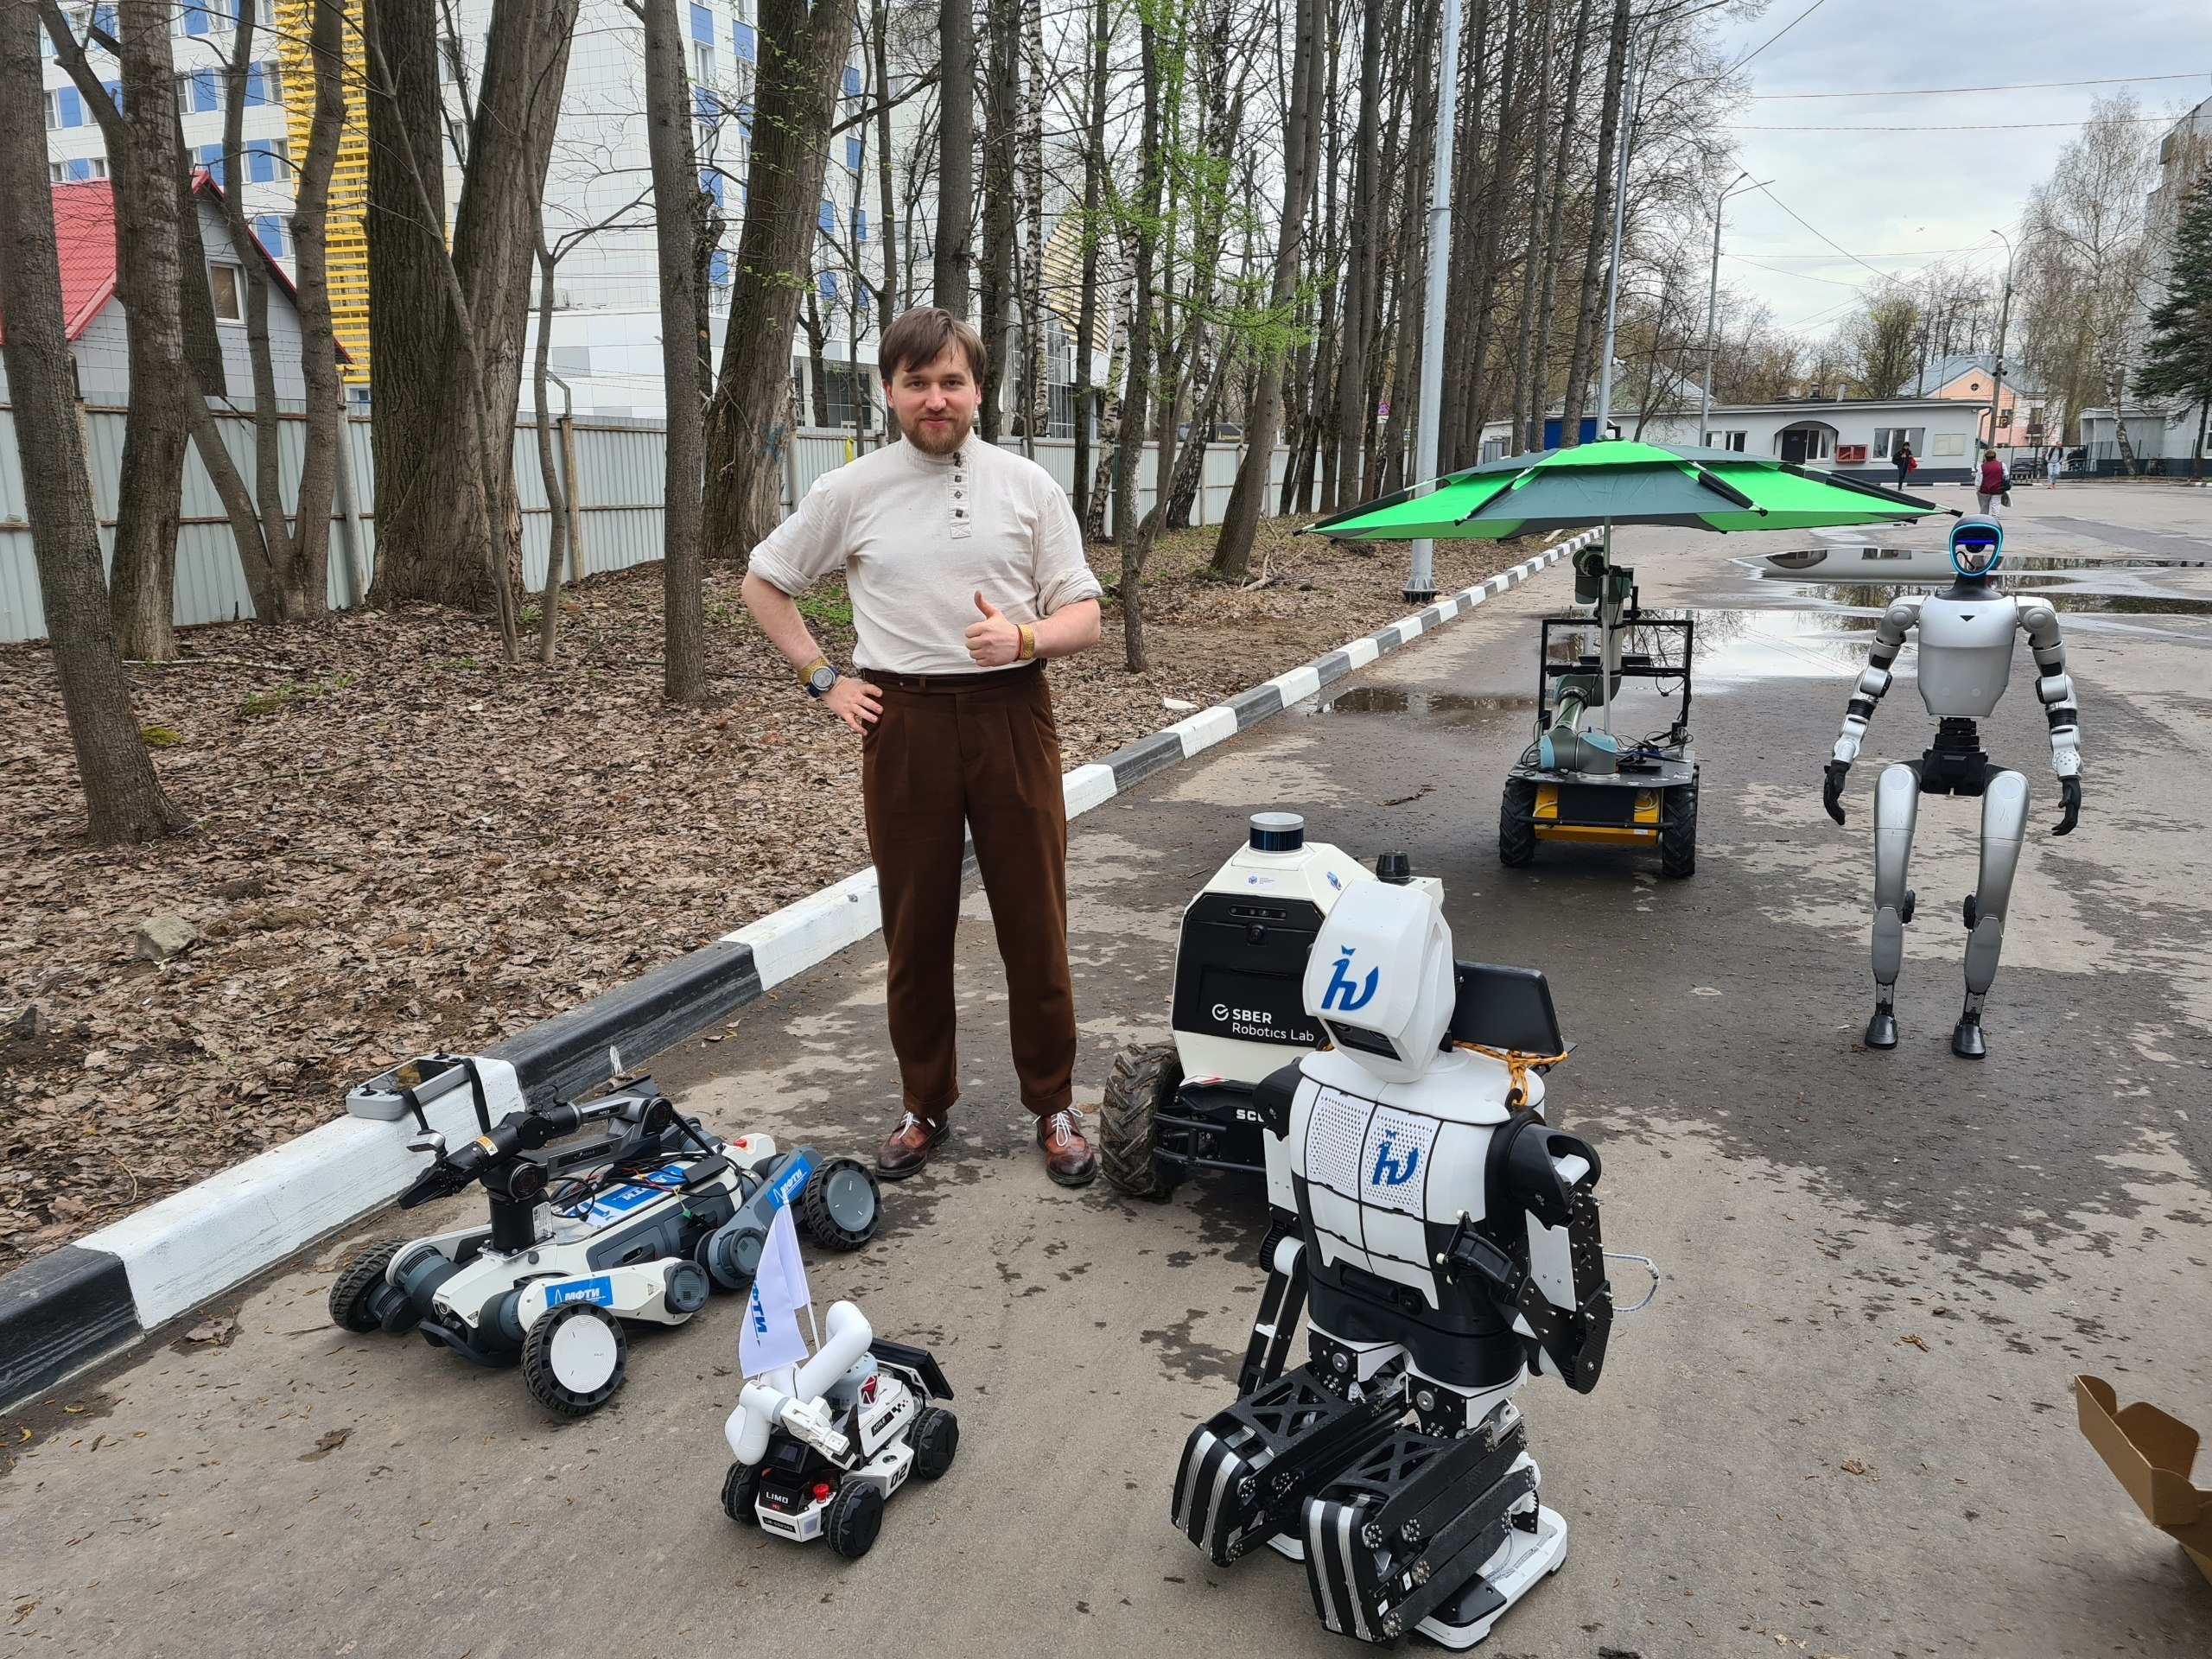
\includegraphics[height=5cm,width=1\textwidth,keepaspectratio]{Oleg.jpg}
                \label{fig:Oleg.jpg}
            \end{figure}
        \end{column}
        \begin{column}{0.49\textwidth}
            \Large
            \vspace{2cm}
            \centering
            \textbf{PhD Oleg Bulichev} \\
            \textit{Mail}: \url{bulichev.ov@mipt.ru}\\
            \textit{TG}: \url{@Lupasic} \\
            \textit{Office Hours}: By request
        \end{column}
    \end{columns}
\end{frame}

\begin{frame}[t]{About Me (2)}
    \framesubtitle{}
    \begin{columns}[T,onlytextwidth]
        \begin{column}{0.69\textwidth}
            \textbf{Education}
            \begin{itemize}
                \item \textit{Bachelor} --- BMSTU (МГТУ им Н.Э. Баумана) <<CAD developer>>
                \item \textit{Master \& PHD} --- Innopolis University (IU) <<Robotics>>
            \end{itemize}
            \textbf{Job}
            \begin{itemize}
                \item \textit{Lead Engineer, Senior Research Fellow} --- MIPT, Center for Cognitive Modeling: SLAM and robotics hardware development
                \item \textit{Associate Professor} --- IU: Supervisor
            \end{itemize}
        \end{column}
        \begin{column}{0.29\textwidth}
            \begin{figure}[H]
                \centering
                \qrcode[height=3cm]{https://t.me/WildOlegAdventures}
                \caption*{\textbf{Link to my channel}}
                \label{fig:qrcode}
            \end{figure}
        \end{column}
    \end{columns}
\end{frame}

\begin{frame}[t]{Why This Course?}
    \framesubtitle{}
    \vspace*{-0.3cm}
    Our laboratory works with AI and has real
    \textbf{robot manipulators} and \textbf{mobile robots}.

    \medskip

    However, using a real robot requires more than developing
    or training an algorithm. We need to understand:
    \begin{itemize}
        \item How robot configuration, pose, and motion are described
        \item What physical and kinematic constraints limit motion
        \item How sensing, noise, synchronization, and calibration
        affect the system
        \item Why singularities, odometry drift, and SLAM failures occur
        \item Where CV, RL, and other AI methods fit into the robot
        architecture
    \end{itemize}

    \medskip

    This course provides the \textbf{robotics foundation}
    needed to work with these systems competently.
\end{frame}

\begin{frame}[c]{Course Goal}
    \framesubtitle{}
    \centering
    \Large

    To develop the \textbf{system-level understanding} \\[0.4em]
    needed to formulate, analyze, and diagnose problems \\
    involving \textbf{robot manipulators} and
    \textbf{mobile robots}, \\[0.4em]
    and to apply CV, RL, and other AI methods \\
    under the \textbf{correct assumptions}

    \bigskip

    \textit{Understand the robotics problem \\
    before choosing the algorithm}
\end{frame}


\begin{frame}[t]{Course Outline}
    \framesubtitle{}
    \small
    \begin{itemize}
        \item \textbf{Robot Manipulators (Weeks 1--5):}
        coordinate frames and transformations, forward and inverse
        kinematics, Jacobians, singularities, parallel robots,
        trajectories, and industrial robot commands

        \item \textbf{Mobile Robots (Weeks 7--9):}
        locomotion mechanisms, differential-drive, Ackermann and
        omnidirectional models, odometry, control tasks, and navigation

        \item \textbf{Sensors, Calibration, and State Estimation (Weeks 10--11):}
        encoders, IMUs, LiDARs, cameras and GNSS; noise,
        synchronization and sensor fusion; intrinsic, extrinsic,
        temporal and hand--eye calibration

        \item[] \textbf{Simultaneous Localization and Mapping (SLAM) (Weeks 12--13):}
        dead reckoning, landmark-based SLAM, pose graphs,
        data association, loop closure, classical and learning-based
        approaches, evaluation metrics, and failure modes
    \end{itemize}
\end{frame}

\begin{frame}[t]{Grading criteria}
    \framesubtitle{}
    \begin{columns}[T,onlytextwidth]
        \begin{column}{0.49\textwidth}
            \textbf{What will be evaluated on the course}
            \begin{itemize}
                \item[Qz:] Quizzes: $20\%$ 
                \item[HWs:] Homework assignments: $40\%$
                \item[HP:] Hardware Projects: $30\%$
                \item[FE:] Final Exam: $10\%$
                \item[Extra:] Slide fixes in Github: $5\%$ 
            \end{itemize}
        \end{column}
        \begin{column}{0.49\textwidth}
            \textbf{Late policy:} -50\% of max grade for a task. One week late is allowed. \\
            \textbf{Scale}:
            \begin{itemize}
                \item[A:] 80 --- 100\%
                \item[B:] 50 --- 79.99\%
                \item[C:] 29.99 --- 49.99\%
                \item[D:] 0 --- 29.99\% or less than $50\%$ by any criterion. 
            \end{itemize}
        \end{column}
    \end{columns}
\end{frame}

\begin{frame}[t]{Quizzes}
    \framesubtitle{}
        \textbf{Purpose}: Quizzes help us to understand what you didn't get during the previous lecture.
        \bigskip

    \textbf{Format}: $5-15\ min$ closed book on a paper sheet, in the beginning of a lecture. \\
    \end{frame}


\begin{frame}[c]{}
    \framesubtitle{}
    \centering \LARGE \textbf{Lab Goals} \\
    Solve math problems on a whiteboard and defend you HWs.
\end{frame}

\begin{frame}[t]{Hardware Projects}
    \framesubtitle{From models to real robotic systems}
    \small

    The course includes three hardware-centered projects:
    \begin{enumerate}
        \item Industrial Manipulator Task Programming
        \item Robot--Camera Calibration and Validation
        \item Mobile Robot Identification, Odometry, and SLAM
    \end{enumerate}

    Each project follows the same engineering workflow:
    \[
        \text{Model}
        \rightarrow
        \text{Configure or calibrate}
        \rightarrow
        \text{Execute}
        \rightarrow
        \text{Measure}
        \rightarrow
        \text{Diagnose}
    \]

\end{frame}

\begin{frame}[t]{Hardware Projects}
\framesubtitle{Organizational problems}
    \begin{itemize}
        \item Three manipulators and three small mobile robots are available
        \item Students may work in teams of two
        \item Each team submits one shared report
        \item Project results are presented and defended as a team
        \item A personal robotic platform may be used with prior approval
    \end{itemize}

    \medskip
    \centering
    \textit{Do not just make the robot work---explain why it works
    and why it fails.}
\end{frame}

\begin{frame}[t]{Project 1: Industrial Manipulator Programming}
    \small
 \vspace*{-0.3cm}
    \textbf{Objective:}
    Program and execute a representative industrial task using
    a real robot manipulator.

    \medskip

    The project includes:
    \begin{itemize}
        \item Defining the base, tool, and work-object coordinate frames
        \item Planning a pick-and-place, inspection, or similar task
        \item Selecting appropriate joint-space and Cartesian-space commands
        \item Using \texttt{MoveJ}, \texttt{MoveL}, and, if supported,
        \texttt{MoveC}
        \item Checking joint limits, singularities, and possible collisions
        \item Comparing planned and observed robot behavior
    \end{itemize}

    \textbf{Result:}
    A working hardware demonstration and a report explaining the
    selected commands, assumptions, limitations, and possible failures.
\end{frame}

\begin{frame}[t]{Project 2: Robot --- Camera Calibration}
    \small
 \vspace*{-0.3cm}
    \textbf{Objective:}
    Solve and validate an eye-in-hand or eye-to-hand calibration problem.

    \medskip

    The project includes:
    \begin{itemize}
        \item Defining all coordinate frames and transformation directions
        \item Collecting measurements from multiple robot poses
        \item Estimating the unknown camera-to-robot transformation
        \item Validating the result using previously unseen poses
        \item Measuring the resulting task-space error
        \item Analyzing the effects of noise, pose selection,
        and incorrect frame conventions
    \end{itemize}

    \textbf{Result:}
    A calibrated robot-camera system that can relate visual observations
    to robot coordinates, together with quantitative validation.
\end{frame}

\begin{frame}[t]{Project 3: Mobile Robot Identification and SLAM}
    \small
    \vspace*{-0.3cm}
    \textbf{Objective:}
    Identify the motion model of a mobile robot and evaluate its
    influence on odometry, localization, and mapping.

    \medskip

    The project includes:
    \begin{itemize}
        \item Identifying kinematic parameters or the relationship
        between commands and robot velocity
        \item Executing and measuring a predefined trajectory
        \item Quantifying odometry error and accumulated drift
        \item Running a localization or SLAM pipeline
        \item Comparing results before and after model identification
    \end{itemize}

    \textbf{Result:}
    A mobile robot demonstration and an evidence-based analysis of the
    difference between predicted, measured, and estimated motion.
\end{frame}


\begin{frame}[t]{Course Materials and Acknowledgements}
    \framesubtitle{}
    \small
    \vspace*{-0.35cm}
    The materials are reorganized and supplemented with the instructor's
    own explanations, examples, and practical assignments and based on the following sources:

    \begin{itemize}
        \item \textbf{Robotics 1 and Robotics 2}
        \\\ Sapienza University of Rome --- Alessandro De Luca

        \item \textbf{Introduction to Robotics}
        \\\ Stanford University --- Oussama Khatib

        \item \textbf{Advanced Robotics Manipulation}
        \\\ Innopolis University --- Alexandr Klimchik

        \item \textbf{Autonomous Mobile Robots}
        \\\ ETH Zürich --- Roland Siegwart, Davide Scaramuzza, and colleagues

        \item \textbf{Modern Robotics: Mechanics, Planning, and Control}
        \\\ Northwestern University --- Kevin M. Lynch and Frank C. Park
    \end{itemize}
\end{frame}

\begin{frame}[t]{What Is a Robot? (1)}
    \framesubtitle{}
    \begin{figure}[H]
        \begin{subfigure}[t]{0.49\textwidth}
            \centering
            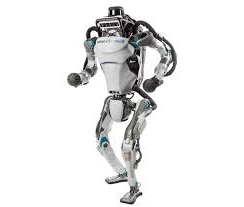
\includegraphics[
                height=6cm,
                width=\textwidth,
                keepaspectratio
            ]{image136.png}
            \label{fig:image136.png}
        \end{subfigure}
        \begin{subfigure}[t]{0.49\textwidth}
            \centering
            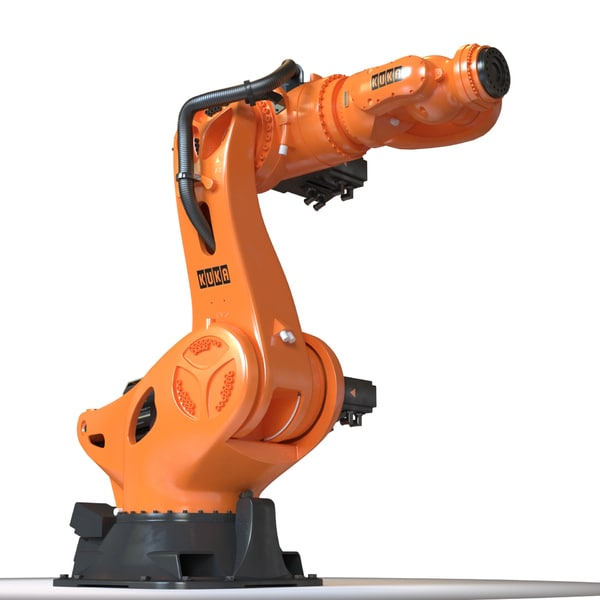
\includegraphics[
                height=6cm,
                width=\textwidth,
                keepaspectratio
            ]{image137.jpg}
            \label{fig:image137.jpg}
        \end{subfigure}
    \end{figure}
\end{frame}


\begin{frame}[t]{What Is a Robot? (2)}
    \framesubtitle{}
    \begin{figure}[H]
        \begin{subfigure}[t]{0.49\textwidth}
            \centering
            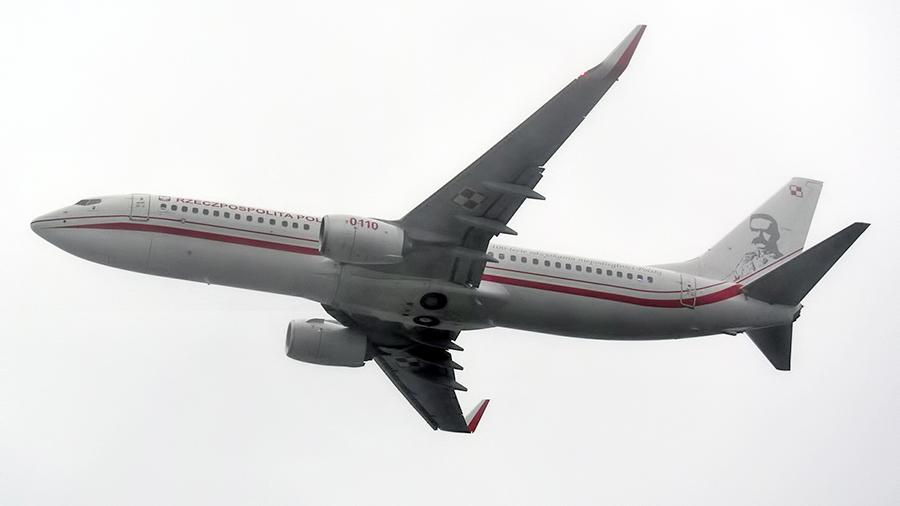
\includegraphics[
                height=3cm,
                width=\textwidth,
                keepaspectratio
            ]{image138.jpg}
            \label{fig:image138.jpg}
        \end{subfigure}
        \begin{subfigure}[t]{0.49\textwidth}
            \centering
            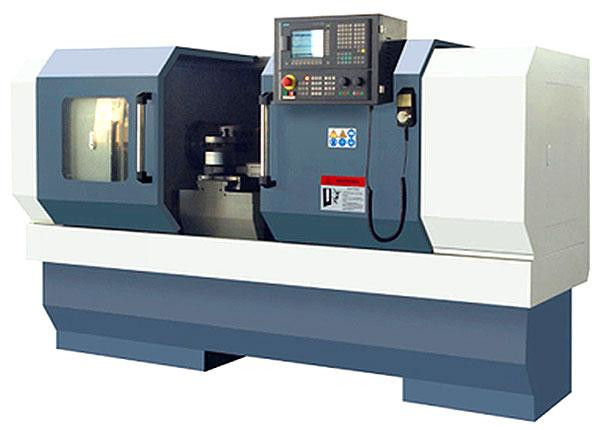
\includegraphics[
                height=3cm,
                width=\textwidth,
                keepaspectratio
            ]{image139.jpg}
            \label{fig:image139.jpg}
        \end{subfigure}

        \begin{subfigure}[t]{0.49\textwidth}
            \centering
            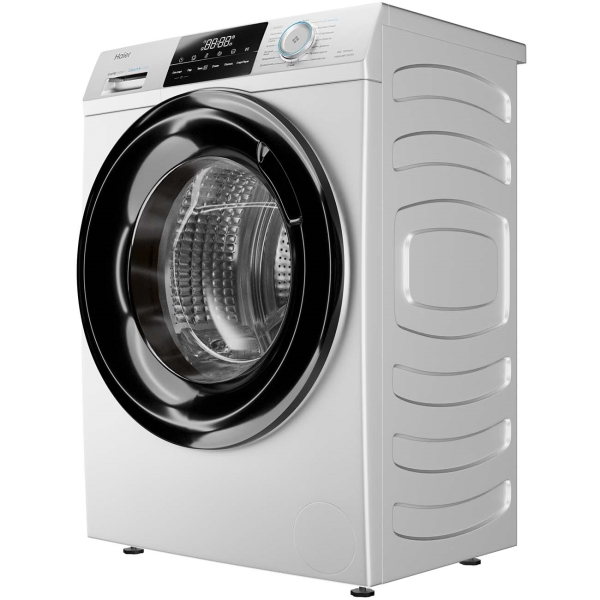
\includegraphics[
                height=3cm,
                width=\textwidth,
                keepaspectratio
            ]{image140.jpg}
            \label{fig:image140.jpg}
        \end{subfigure}
        \begin{subfigure}[t]{0.49\textwidth}
            \centering
            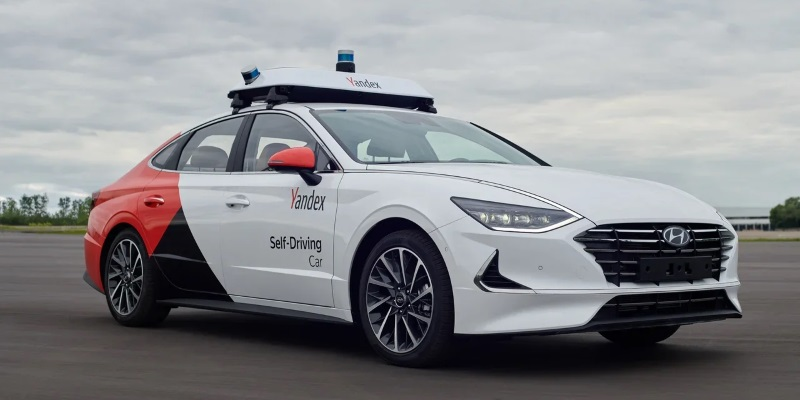
\includegraphics[
                height=3cm,
                width=\textwidth,
                keepaspectratio
            ]{image141.jpg}
            \label{fig:image141.jpg}
        \end{subfigure}
    \end{figure}
\end{frame}


\begin{frame}[t]{What Is a Robot? (3)}
    \framesubtitle{}
    \vspace*{-0.3cm}
    \only<1->{%
        \begin{block}{Wikipedia}
            \raggedright
            A robot is an automatic device designed to perform various
            mechanical operations according to a predefined program.
        \end{block}
    }

    \vspace*{-0.3cm}

    \only<2->{%
        \begin{flushright}
            \begin{block}{GOST R 60.0.0.4-2019}
                \raggedleft
                An actuated mechanism programmable in two or more axes,
                possessing a degree of autonomy and capable of moving within
                its environment to perform intended tasks.
            \end{block}
        \end{flushright}
    }

    \vspace*{-0.8cm}

    \only<3->{%
        \begin{block}{ISO/TC 299}
            \raggedright
            A programmable actuated mechanism with a degree of autonomy
            that performs locomotion, manipulation, or positioning.
        \end{block}
    }
\end{frame}

\begin{frame}[t]{New standards}
\framesubtitle{}
    \vspace{-0.6cm}
    \begin{figure}[H]
        \centering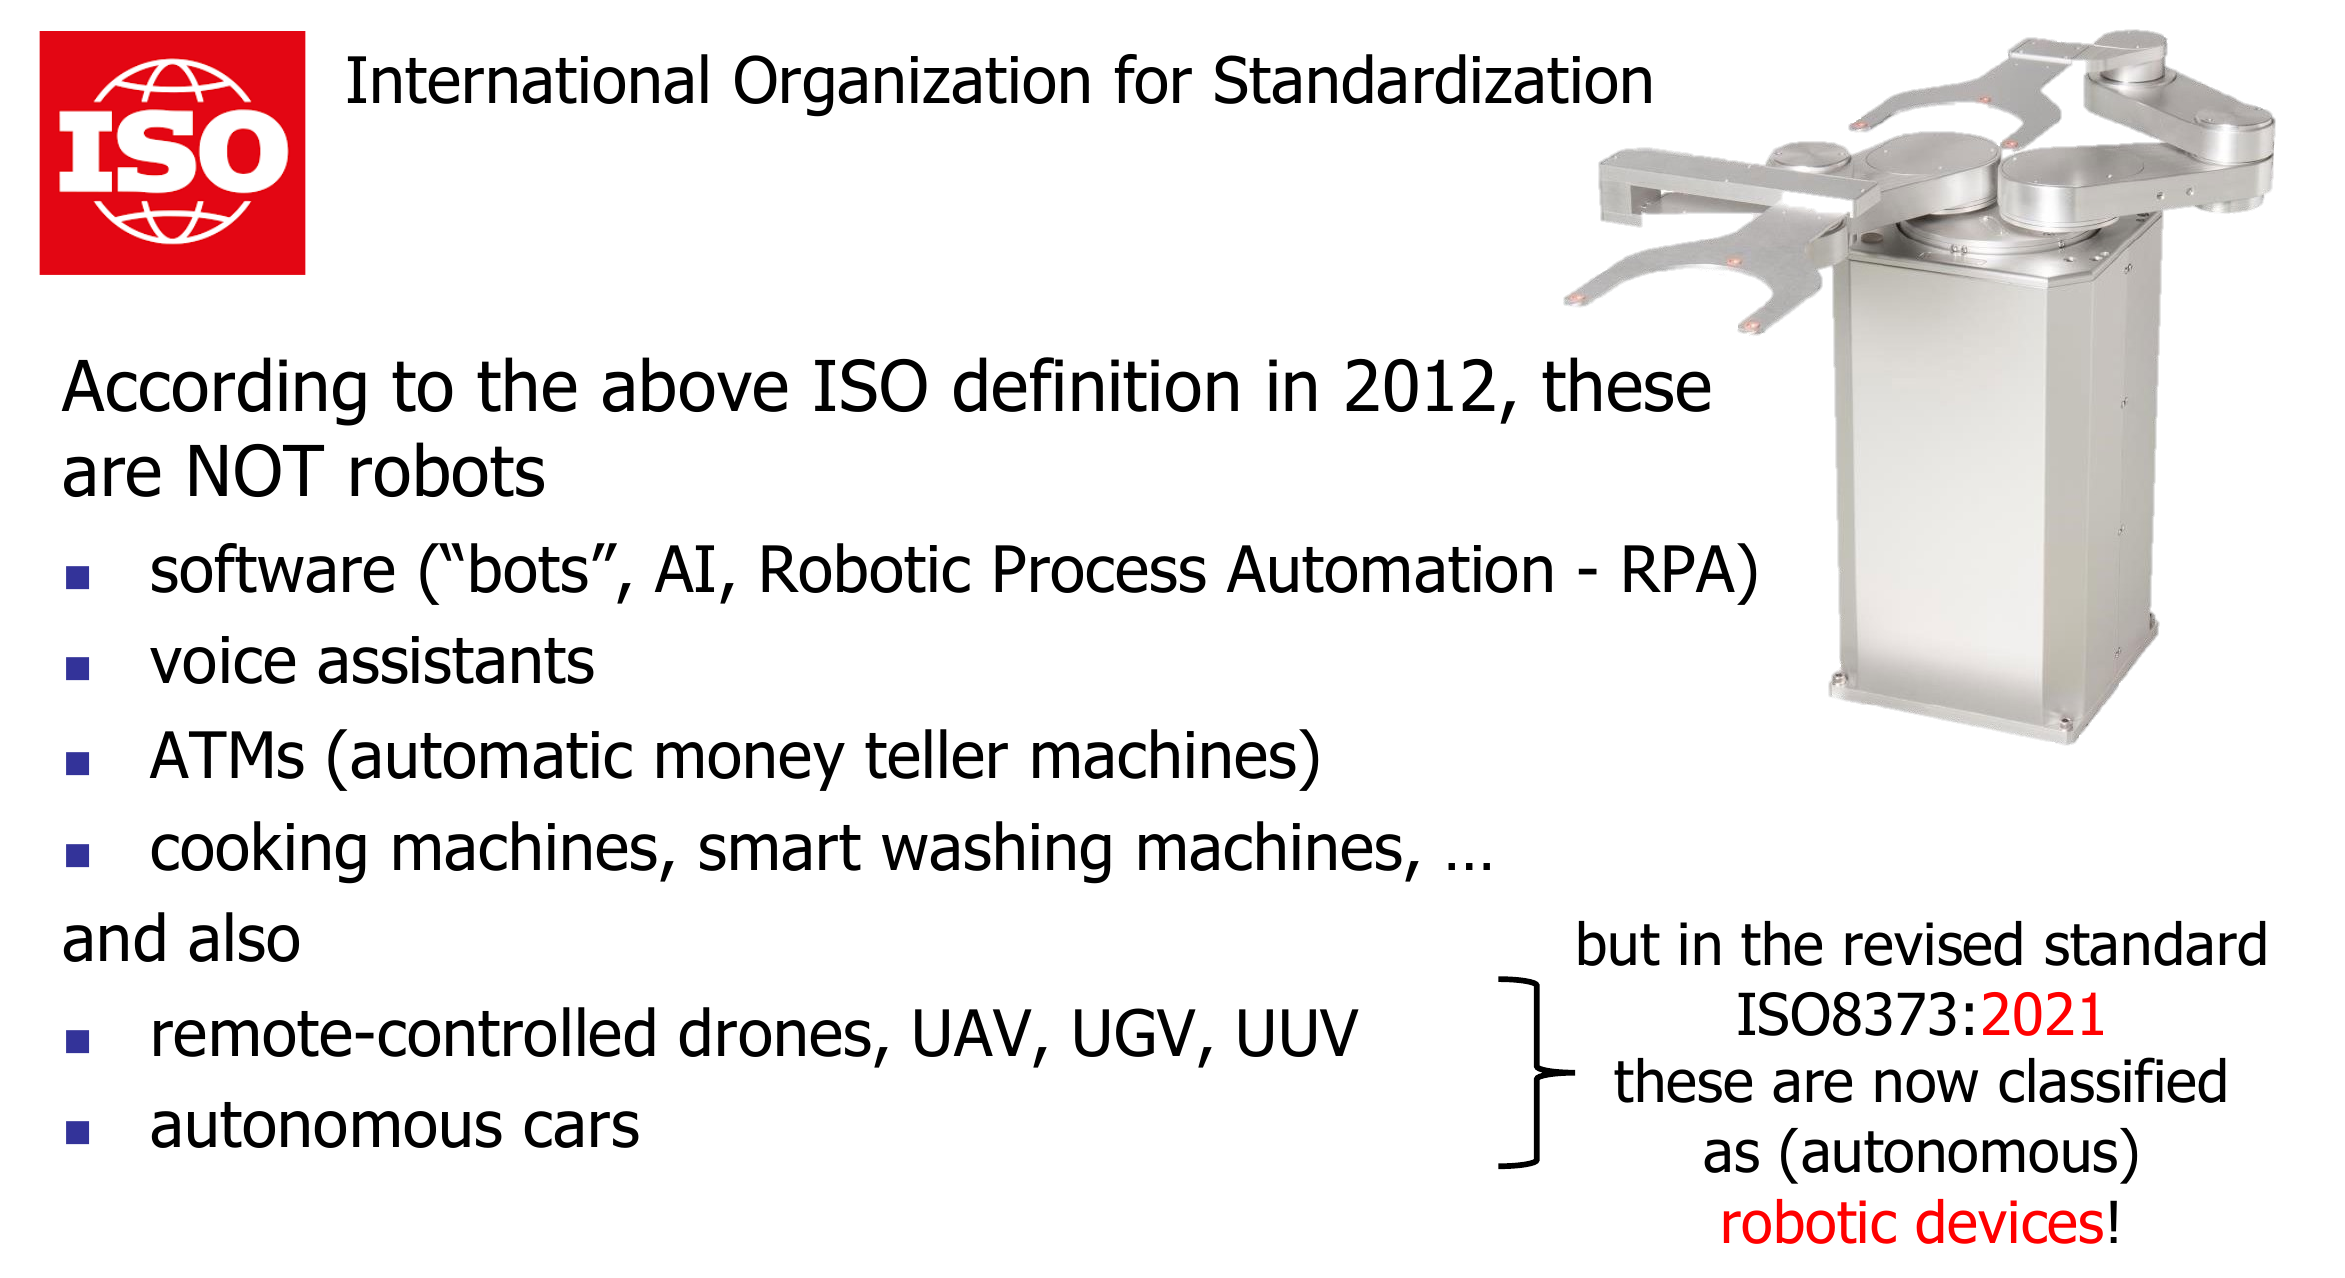
\includegraphics[height=6cm,width=1\textwidth,keepaspectratio]{de_luca_01_industrialrobots_p04.png}
        \label{fig:de_luca_01_industrialrobots_p04.png}
    \end{figure}
\end{frame}



\begin{frame}[t]{The word robot began as cultural imagination}
            \centering
            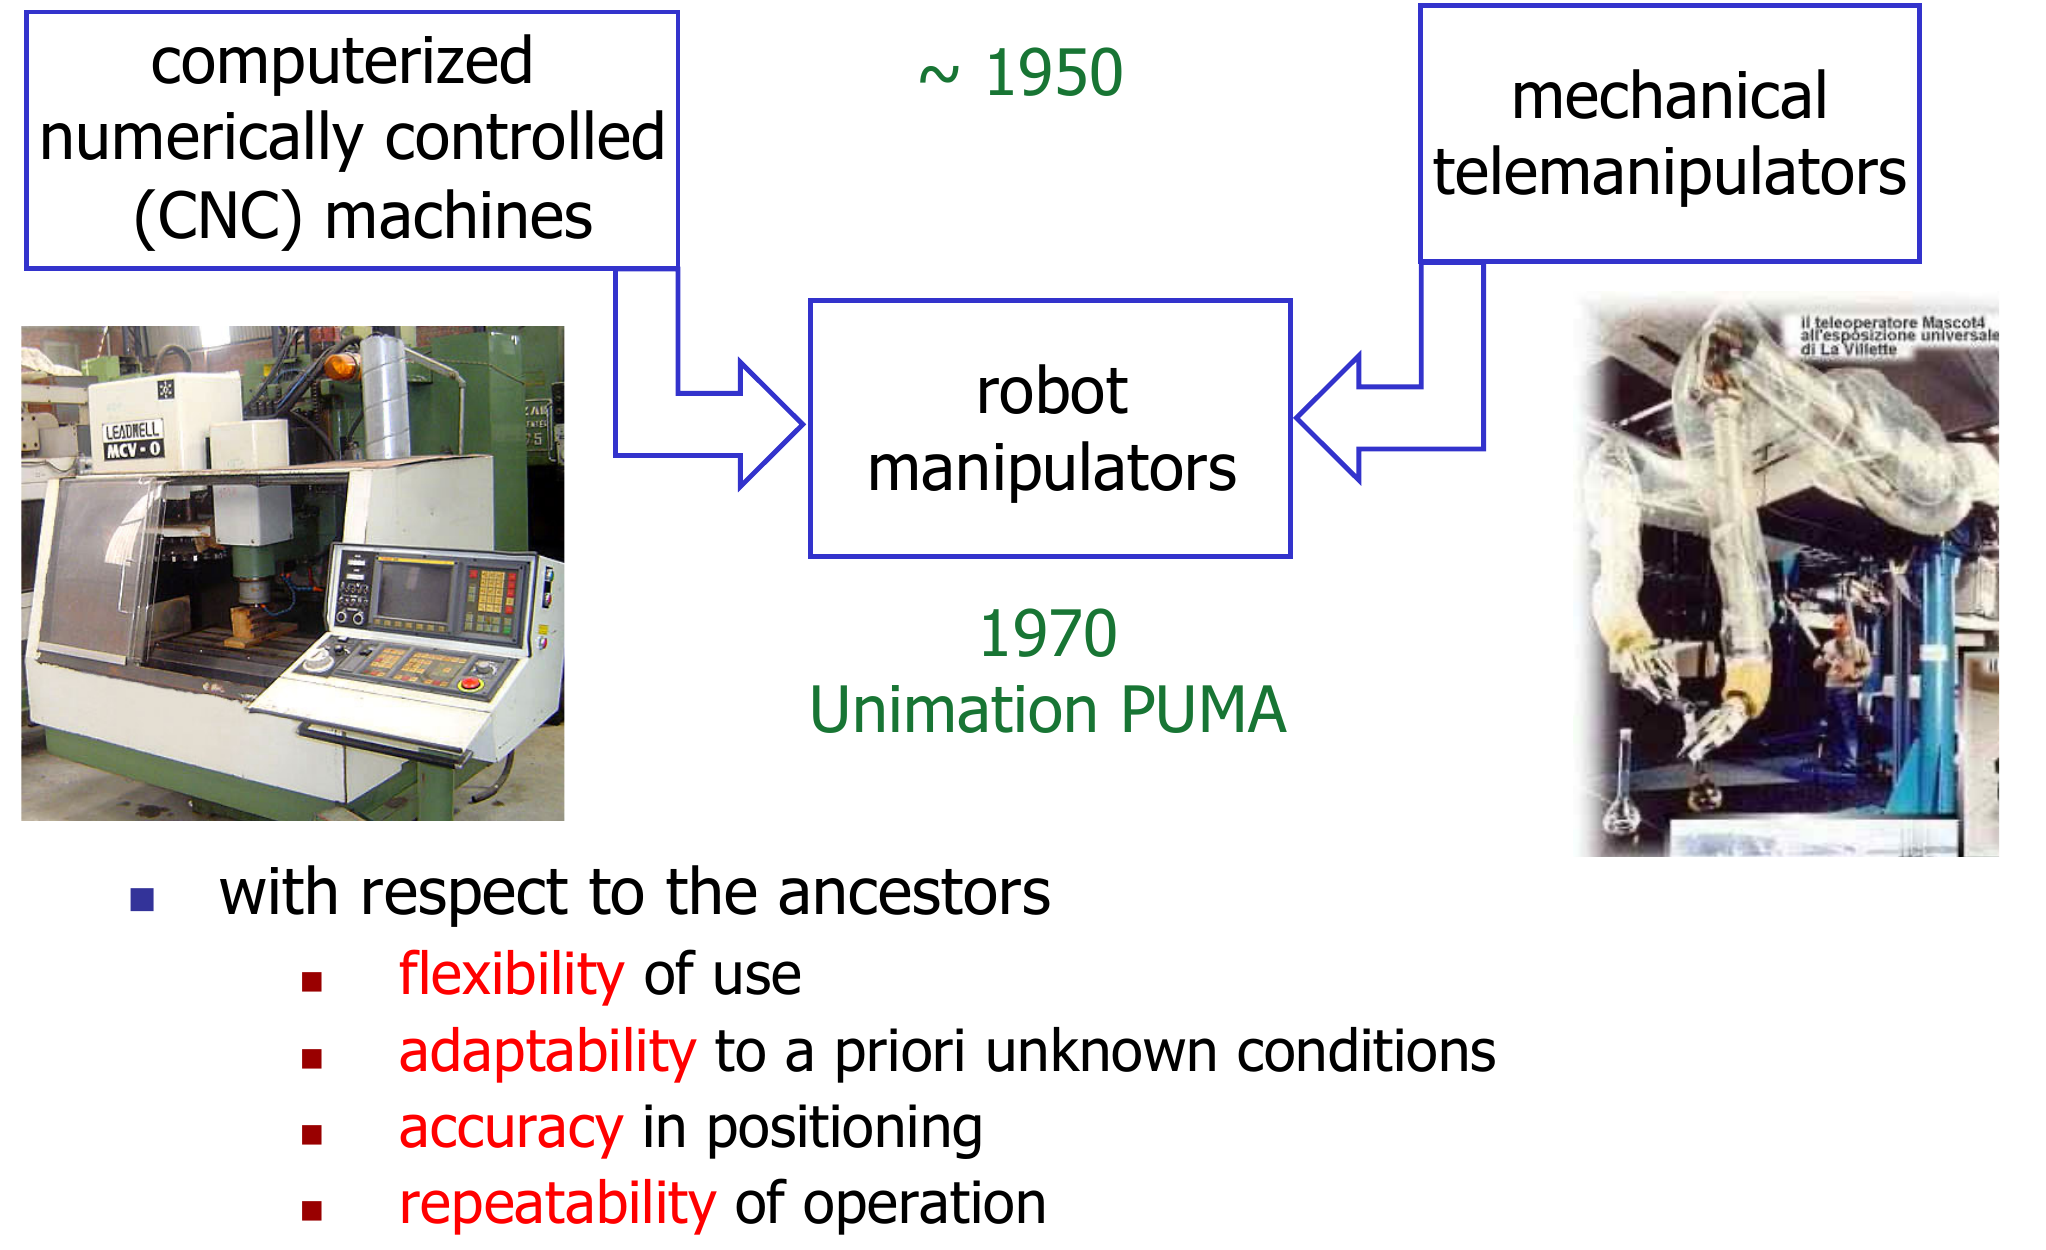
\includegraphics[
                width=\linewidth,
                height=.66\textheight,
                keepaspectratio
            ]{source_native/de_luca/de_luca_01_industrialrobots_p06.png}

\end{frame}


\begin{frame}[t]{An industrial robot system is more than an arm}
            \centering
            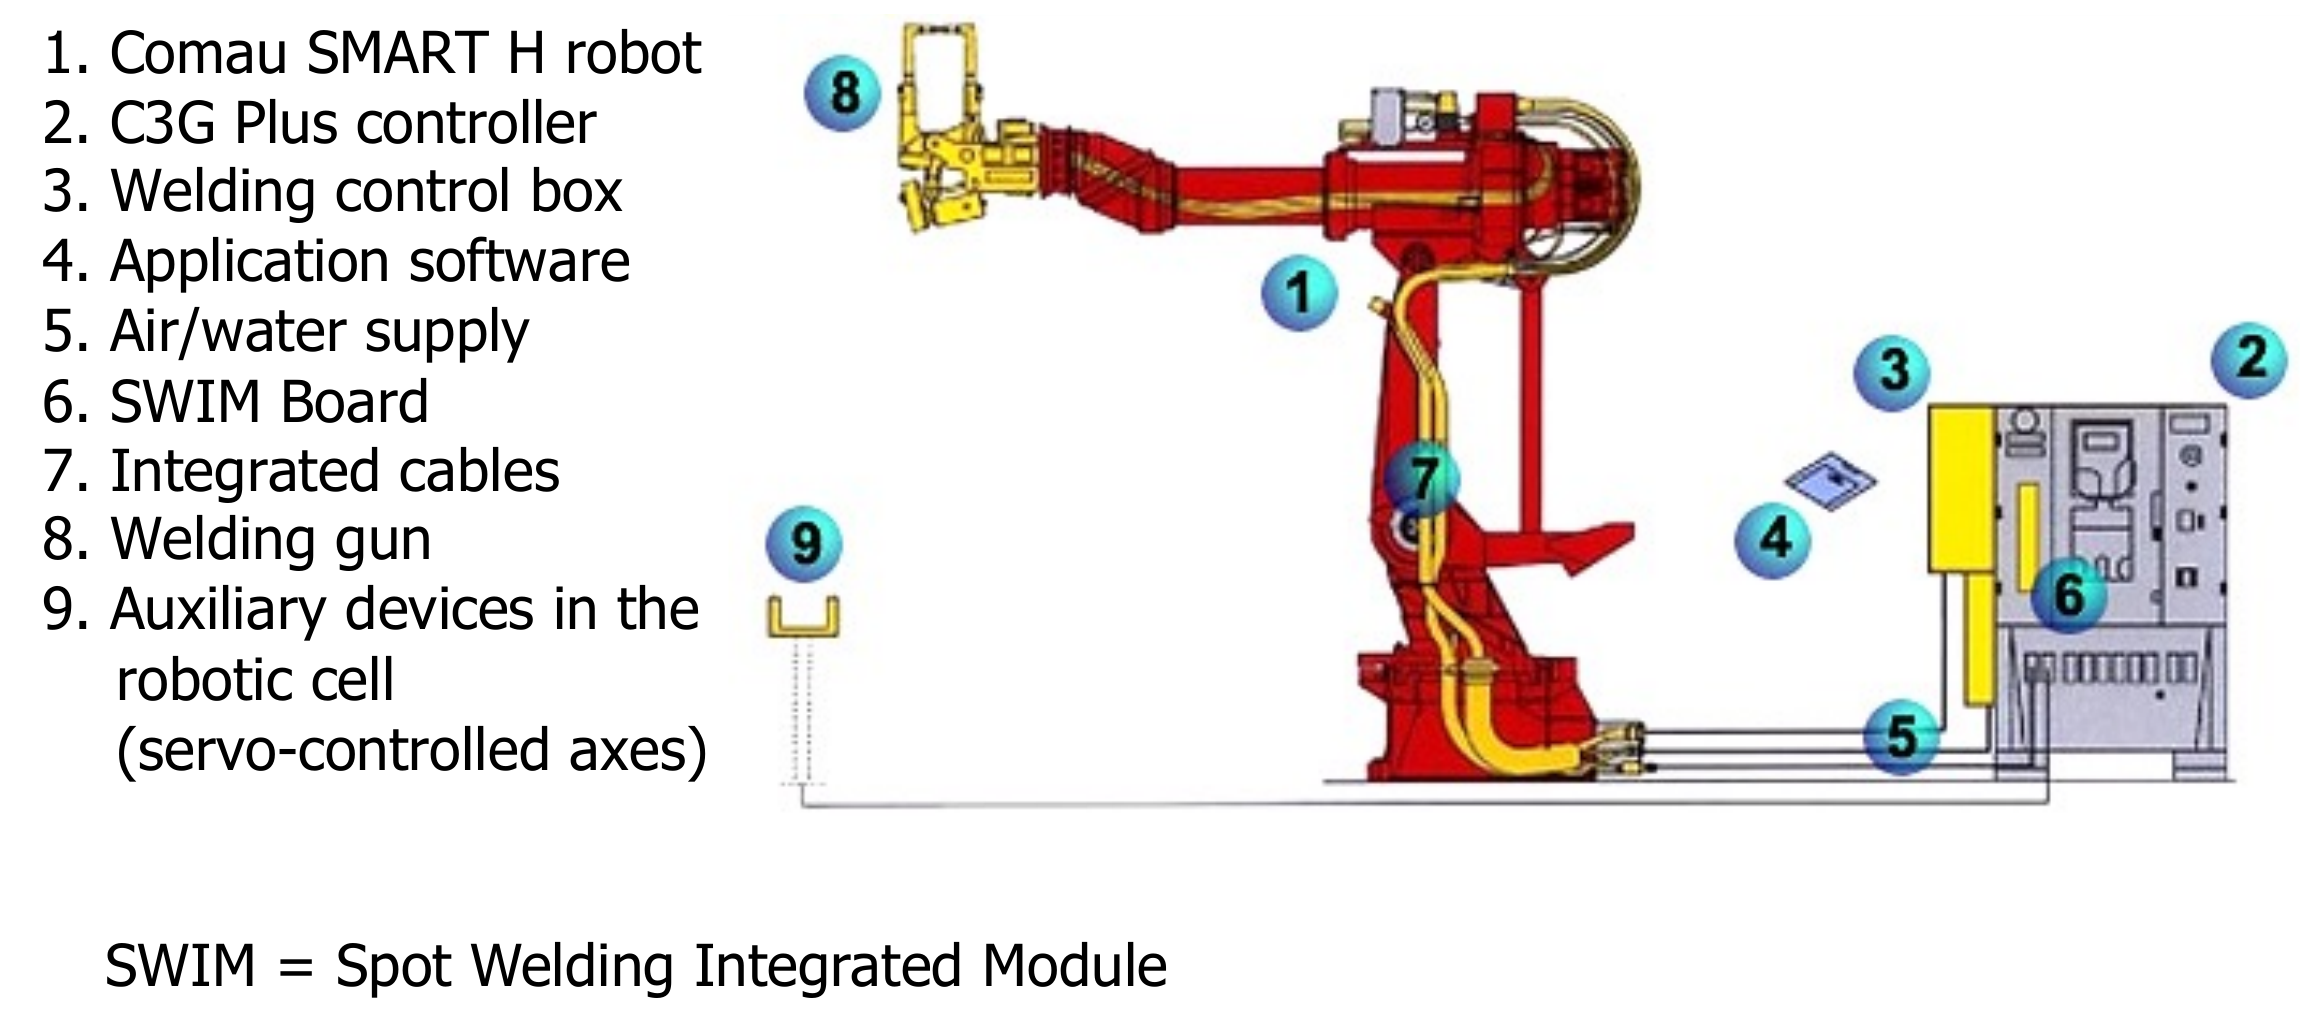
\includegraphics[
                width=\linewidth,
                height=.66\textheight,
                keepaspectratio
            ]{source_native/de_luca/de_luca_01_industrialrobots_p26.png}
\end{frame}

\begin{frame}[t]{Industrial tasks impose different constraints}
	\begin{columns}[T,onlytextwidth]
		\begin{column}{.5\textwidth}
			\centering
			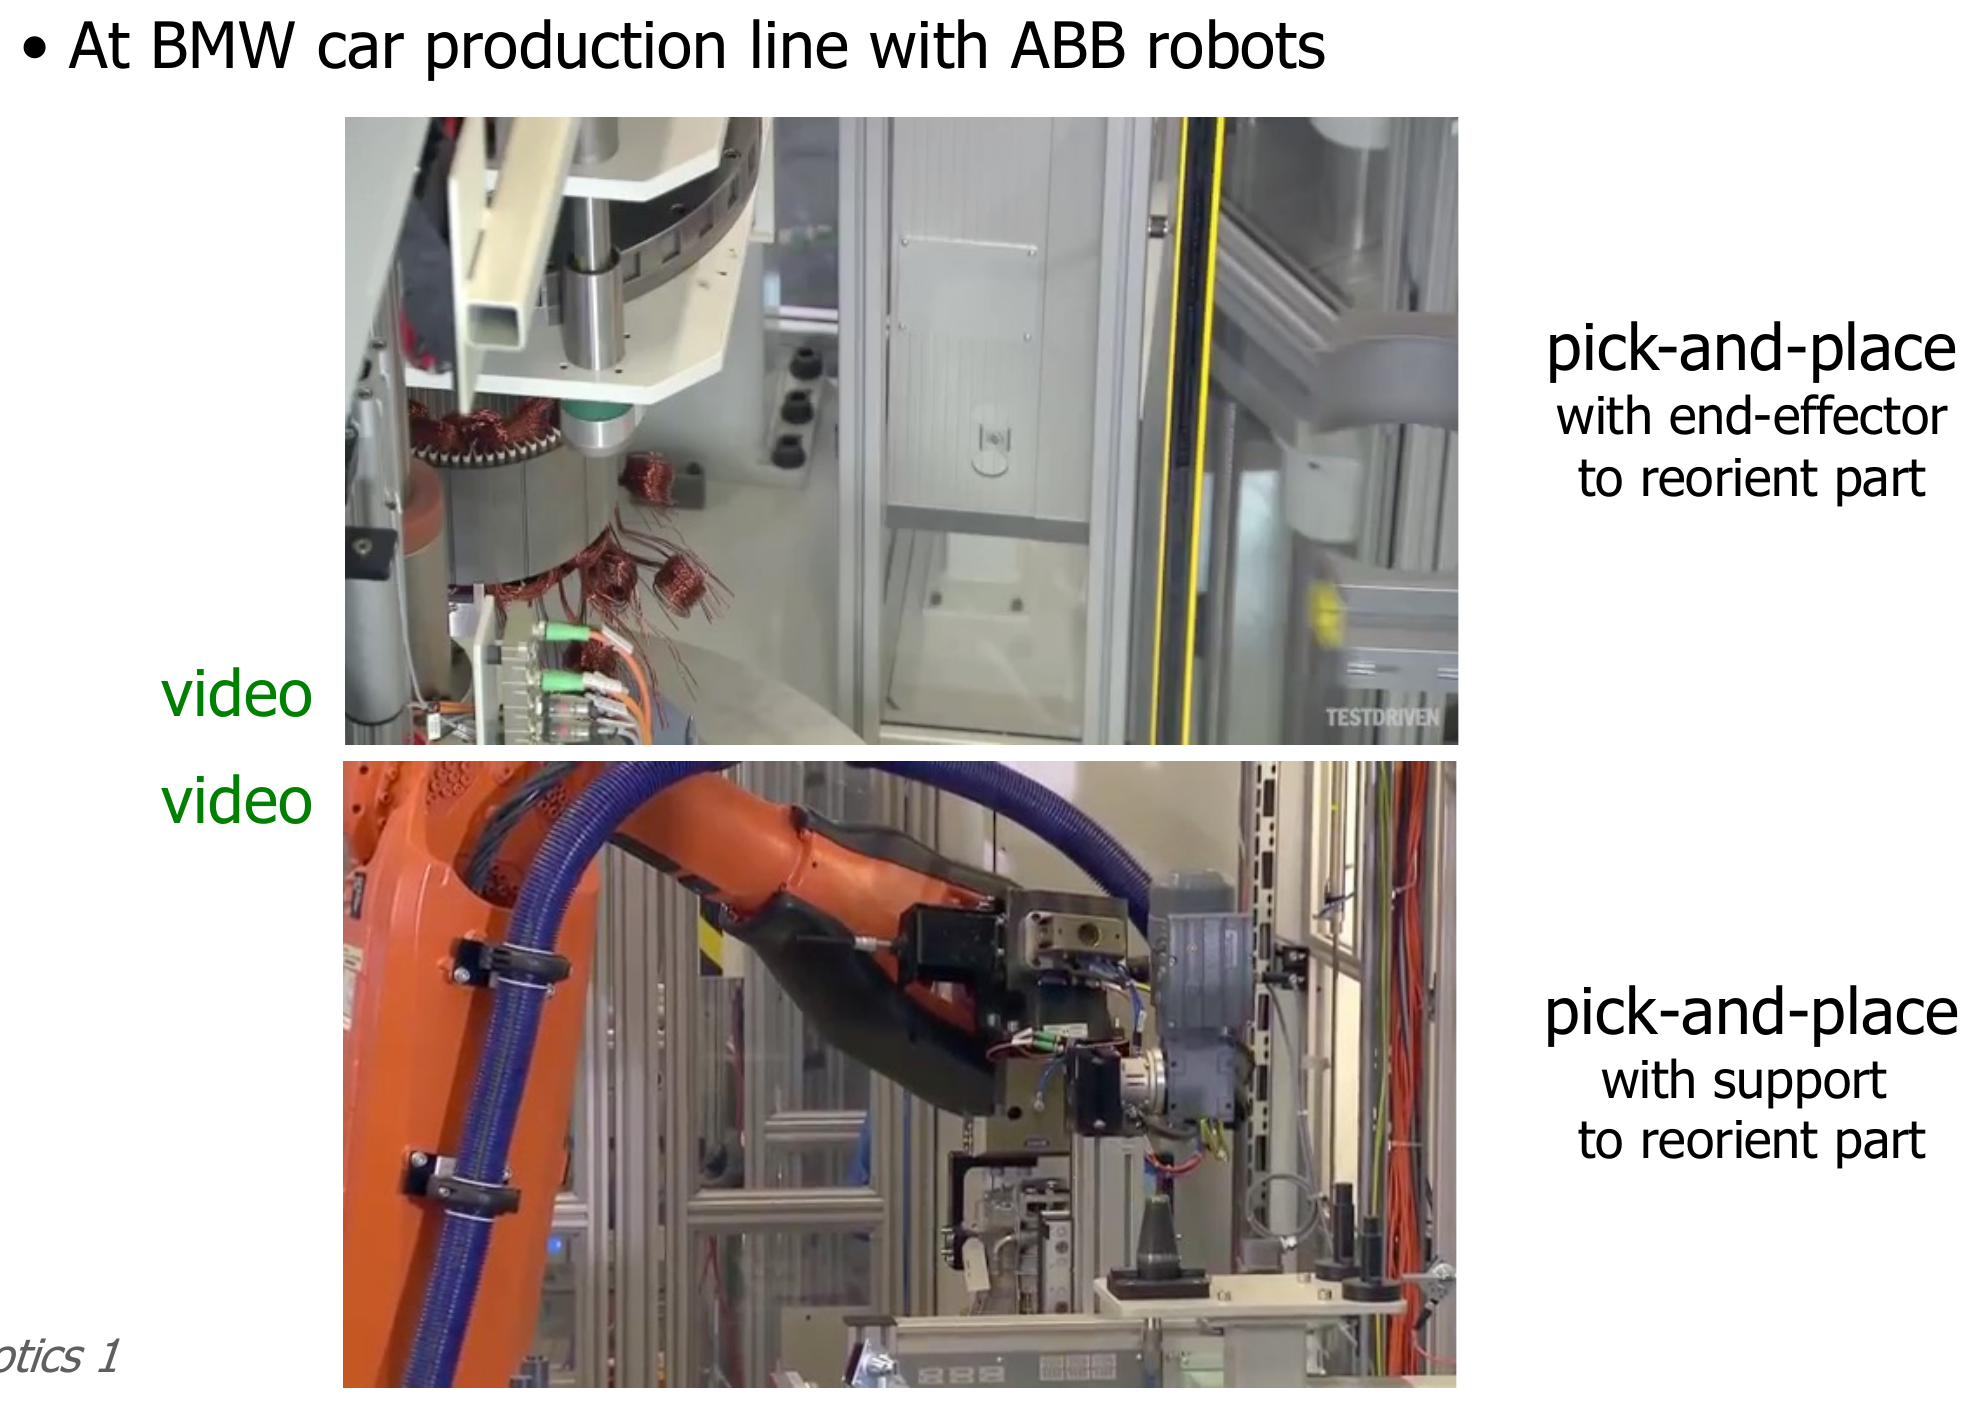
\includegraphics[width=\linewidth,height=.56\textheight,keepaspectratio]{source_native/de_luca/de_luca_01_industrialrobots_p29.png}
		\end{column}
		\begin{column}{.5\textwidth}
			\centering
			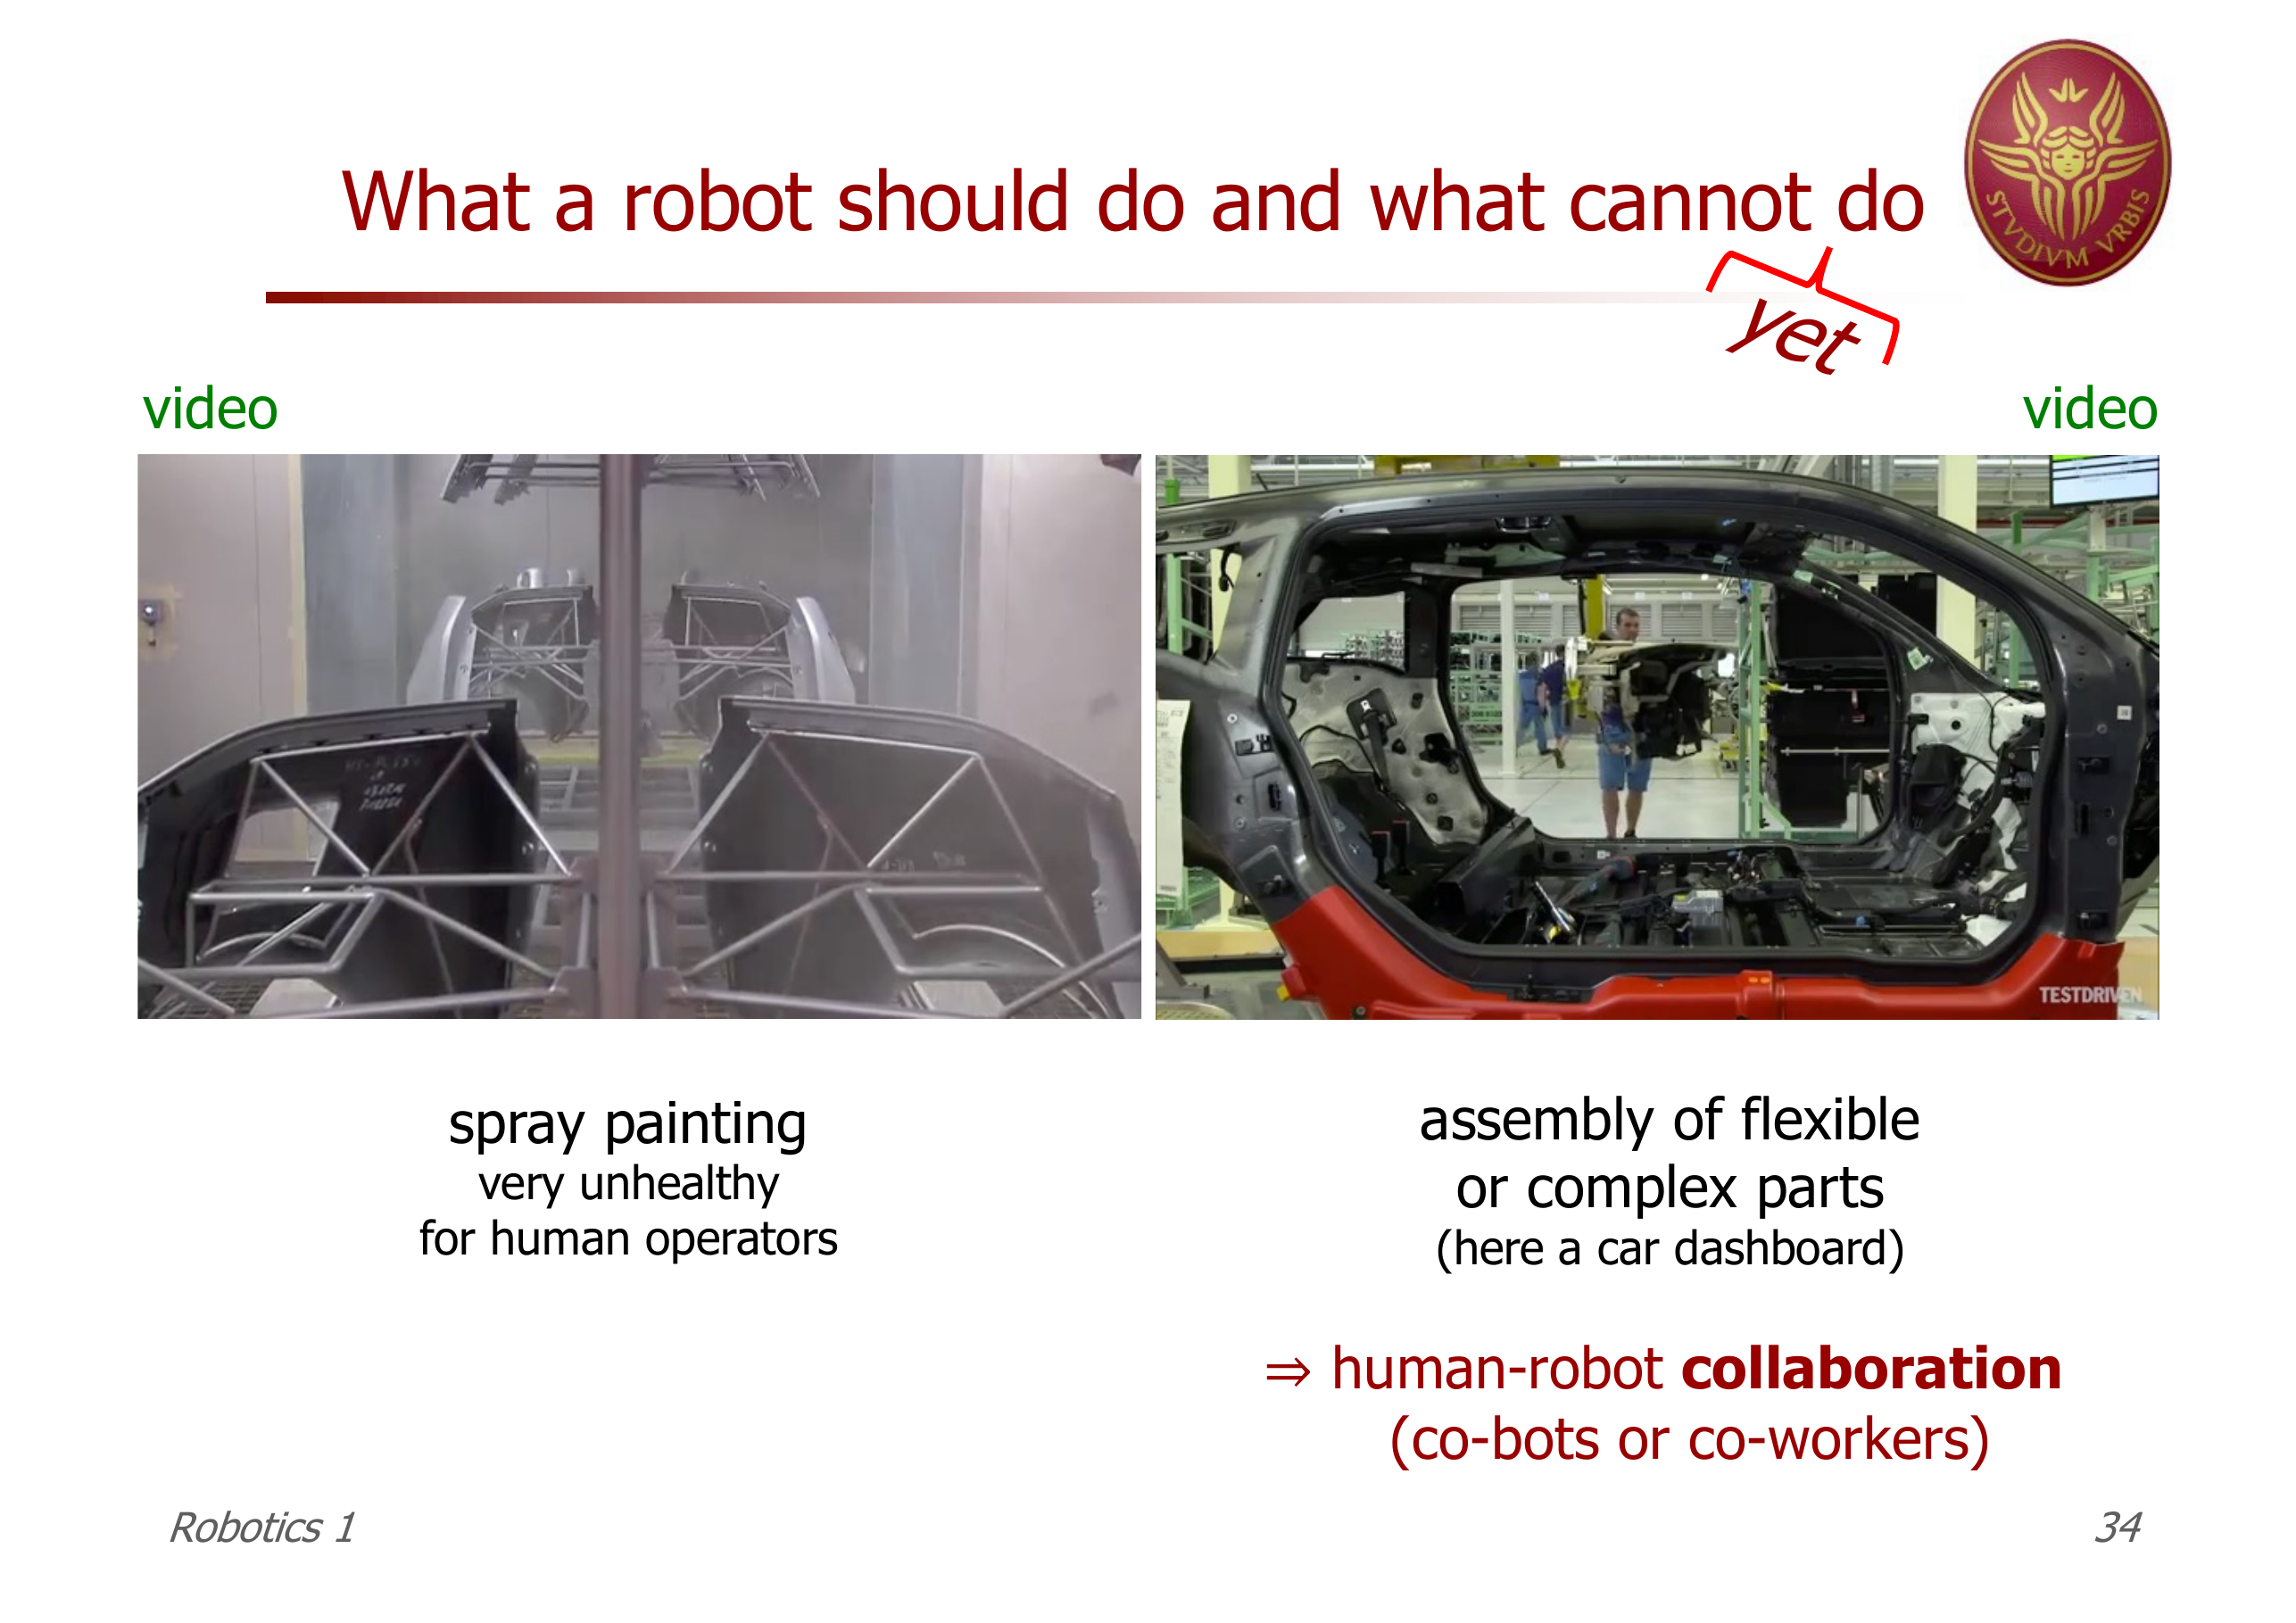
\includegraphics[width=\linewidth,height=.56\textheight,keepaspectratio]{source_native/de_luca/de_luca_01_industrialrobots_p34.png}
		\end{column}
	\end{columns}
	\small Manipulation, assembly, packaging, coating, welding, machining, inspection, and HRC are source examples, not universal capability evidence.
\end{frame}


\begin{frame}[t]{Mobile Robots in Real-World Applications}
    \framesubtitle{}
    \vspace{-0.4cm}
    \begin{figure}[H]
        \begin{subfigure}[t]{0.49\textwidth}
            \centering
            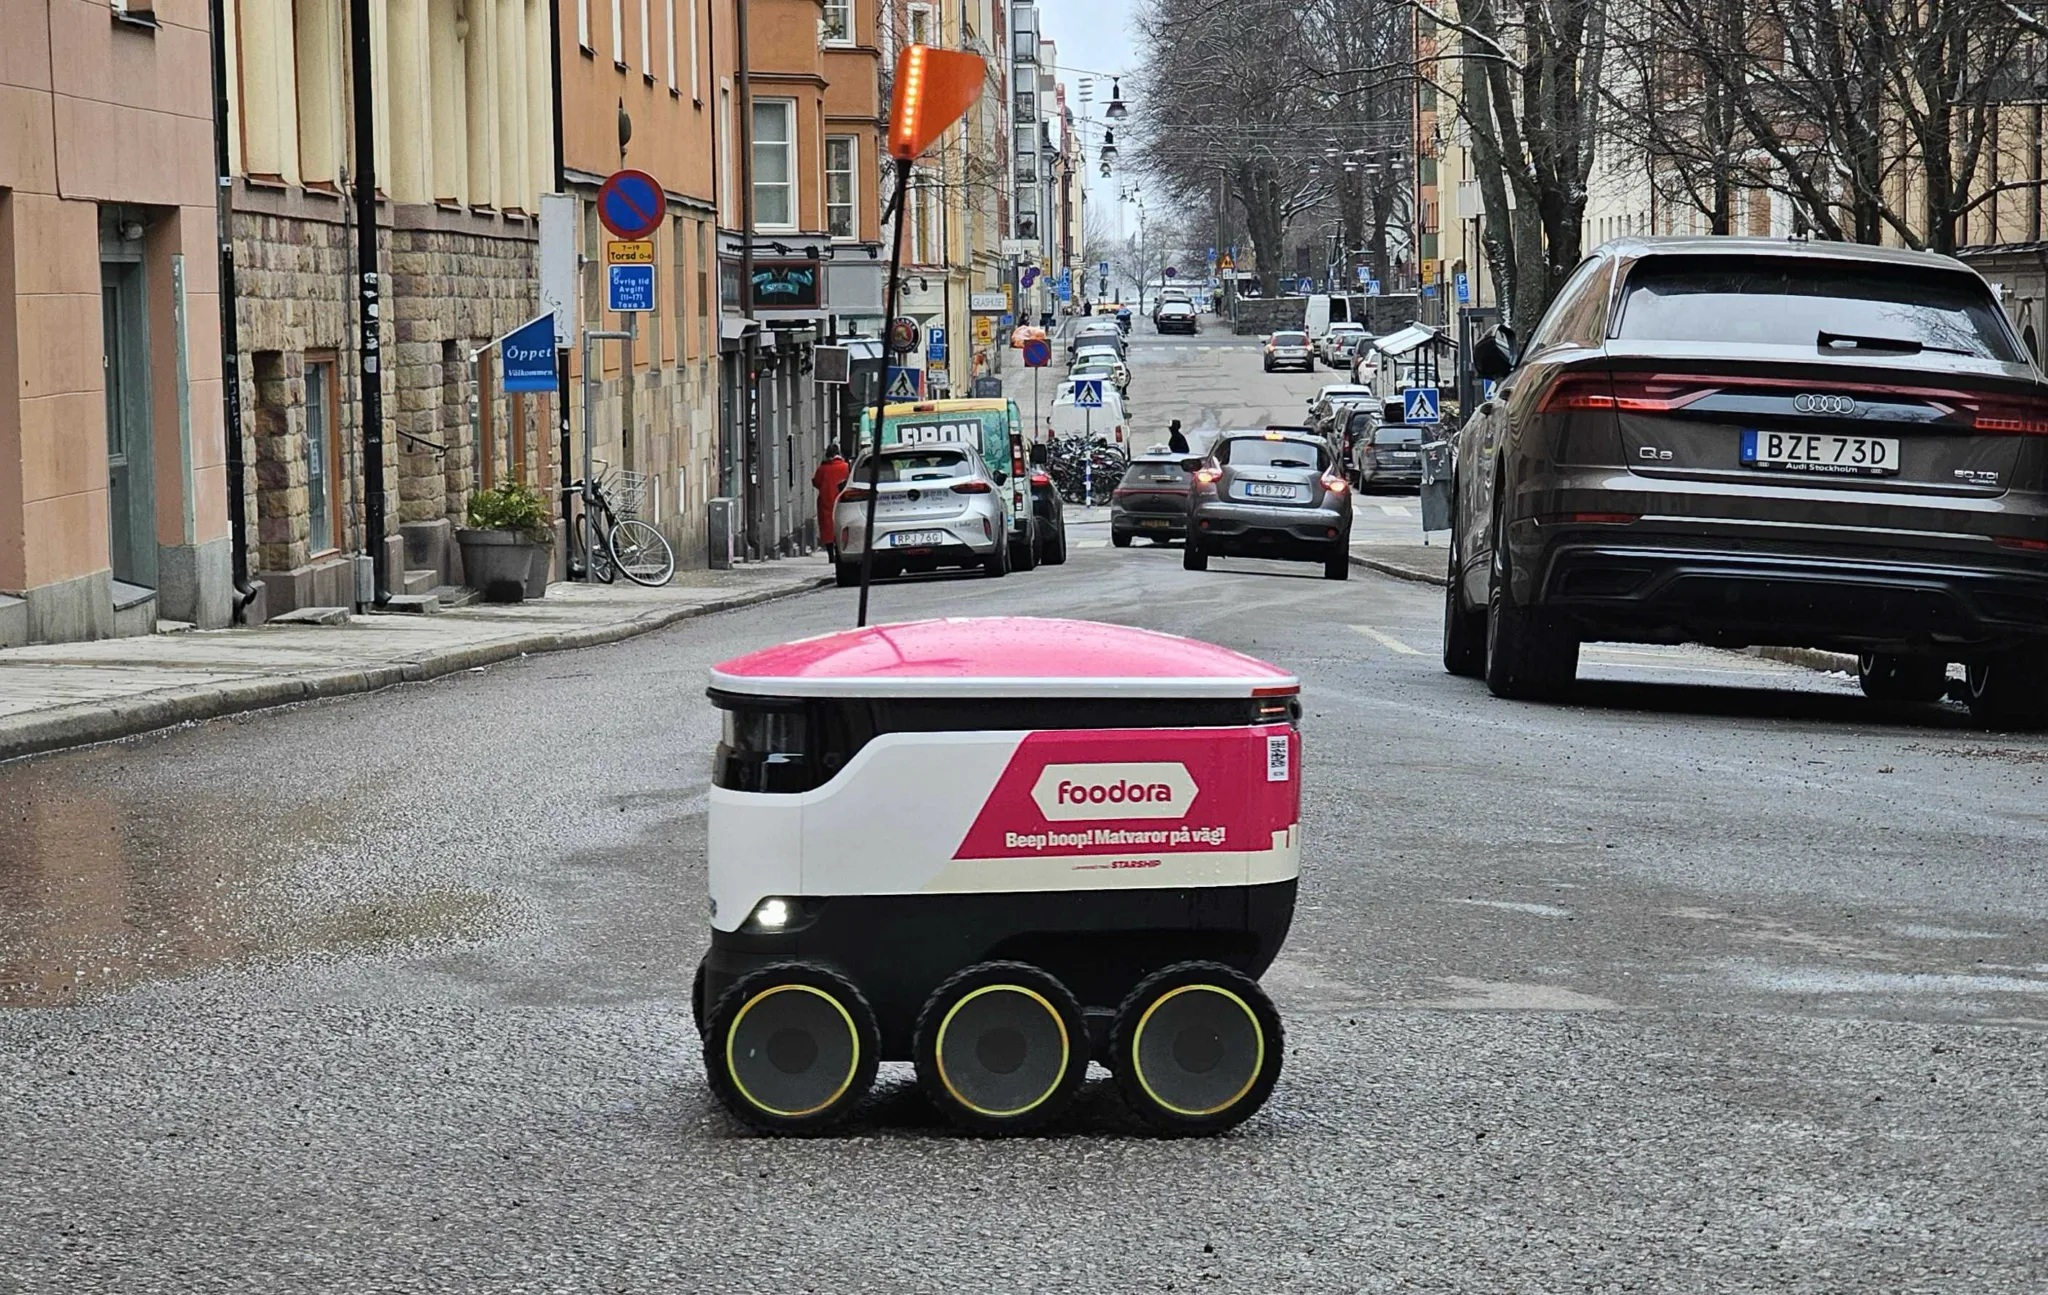
\includegraphics[height=1.9cm,width=\textwidth,keepaspectratio]{applications/starship_delivery.jpg}
            \\[-0.1em]\textbf{Delivery}
            \\[-0.2em]{\scriptsize Starship Technologies}
        \end{subfigure}
        \begin{subfigure}[t]{0.49\textwidth}
            \centering
            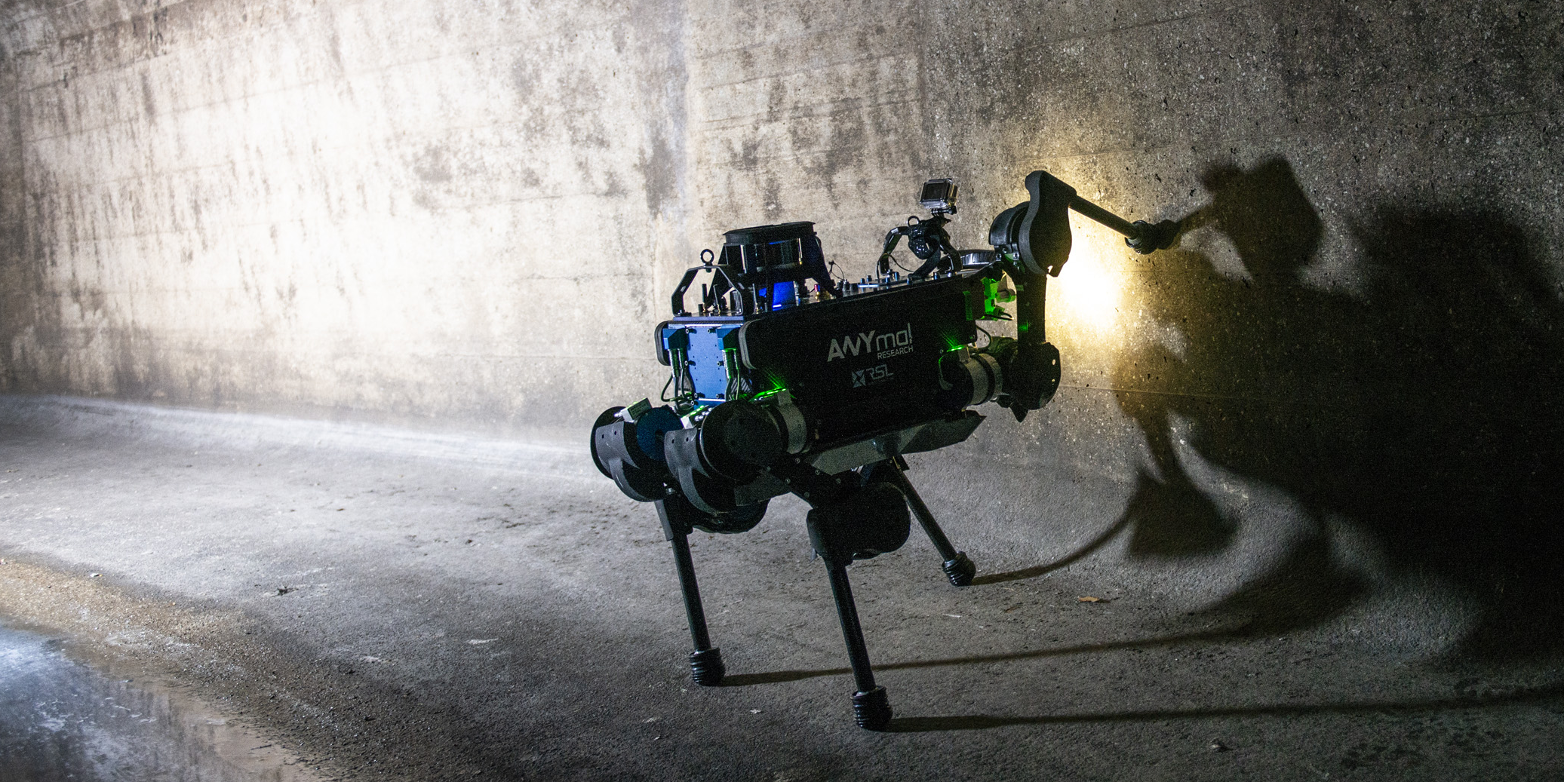
\includegraphics[height=1.9cm,width=\textwidth,keepaspectratio]{applications/anymal_inspection.png}
            \\[-0.1em]\textbf{Inspection}
            \\[-0.2em]{\scriptsize ANYmal, ETH Zurich}
        \end{subfigure}

        \vspace{0.05cm}

        \begin{subfigure}[t]{0.49\textwidth}
            \centering
            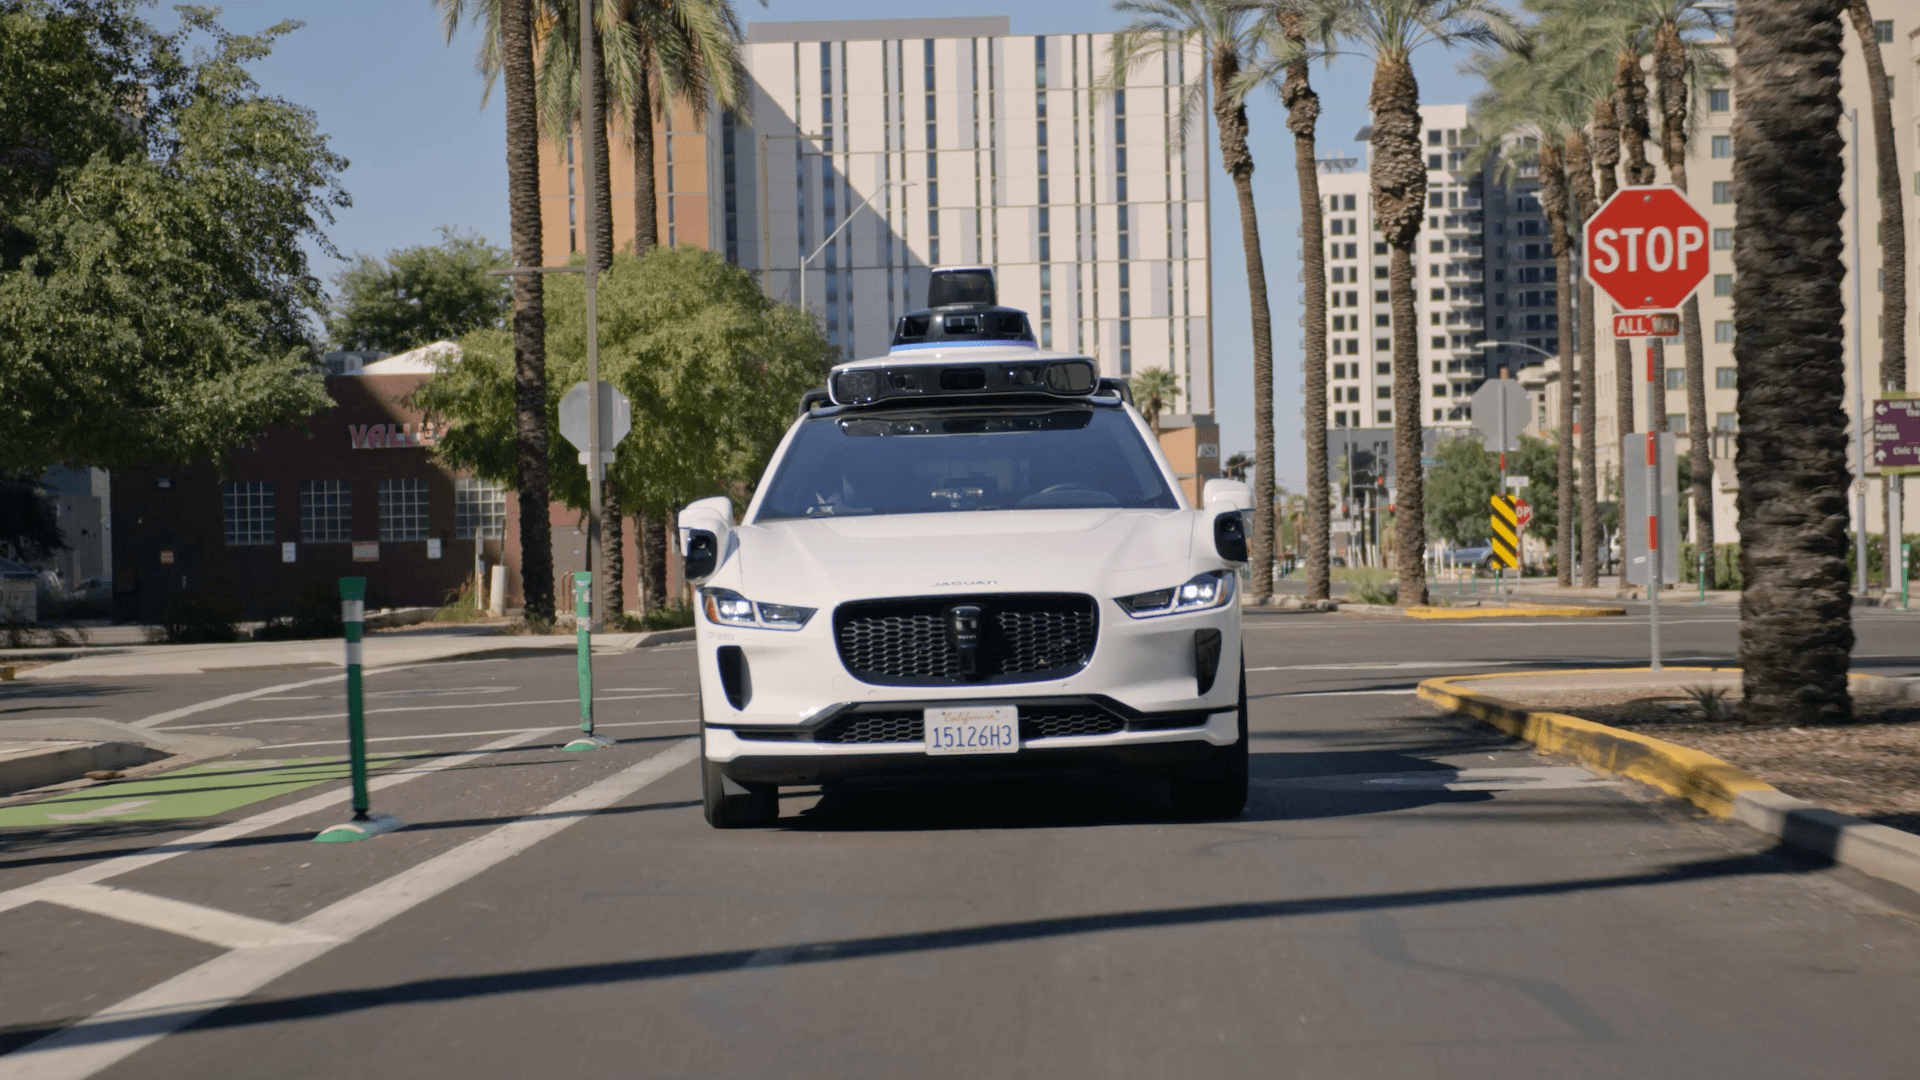
\includegraphics[height=1.9cm,width=\textwidth,keepaspectratio]{applications/waymo_transport.jpg}
            \\[-0.1em]\textbf{Transportation}
            \\[-0.2em]{\scriptsize Waymo}
        \end{subfigure}
        \begin{subfigure}[t]{0.49\textwidth}
            \centering
            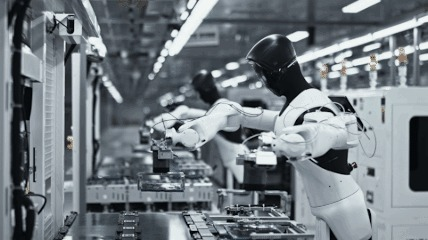
\includegraphics[height=1.9cm,width=\textwidth,keepaspectratio]{applications/agibot_frame_038.jpg}
            \\[-0.1em]\textbf{Mobile manipulation}
            \\[-0.2em]{\scriptsize AGIBOT G2}
        \end{subfigure}
    \end{figure}
\end{frame}

\begin{frame}[t]{Mobile robot with manipulator}
\framesubtitle{}
    \begin{figure}[H]
        \begin{subfigure}[t]{0.39\textwidth}
            \centering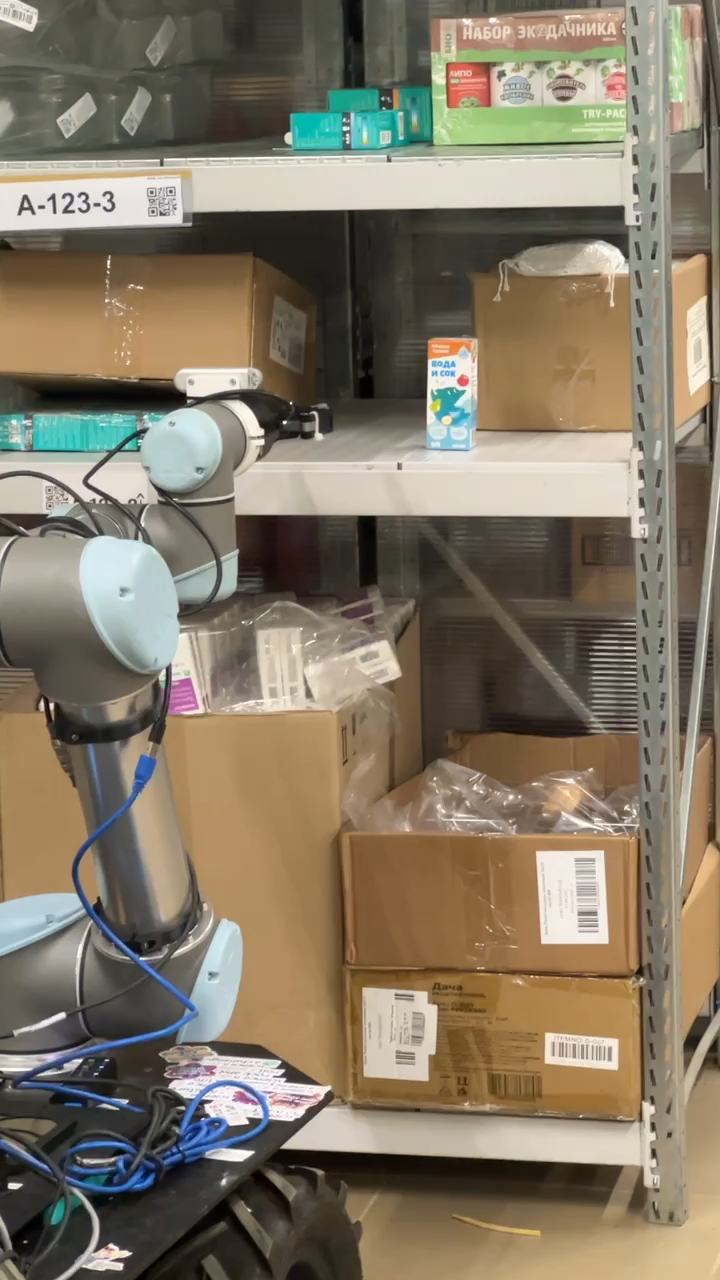
\includegraphics[height=6cm,width=1\textwidth,keepaspectratio]{video_2026-01-19_13-08-35.png}
            \label{fig:video_2026-01-19_13-08-35.png}
        \end{subfigure}
        \begin{subfigure}[t]{0.59\textwidth}
            \centering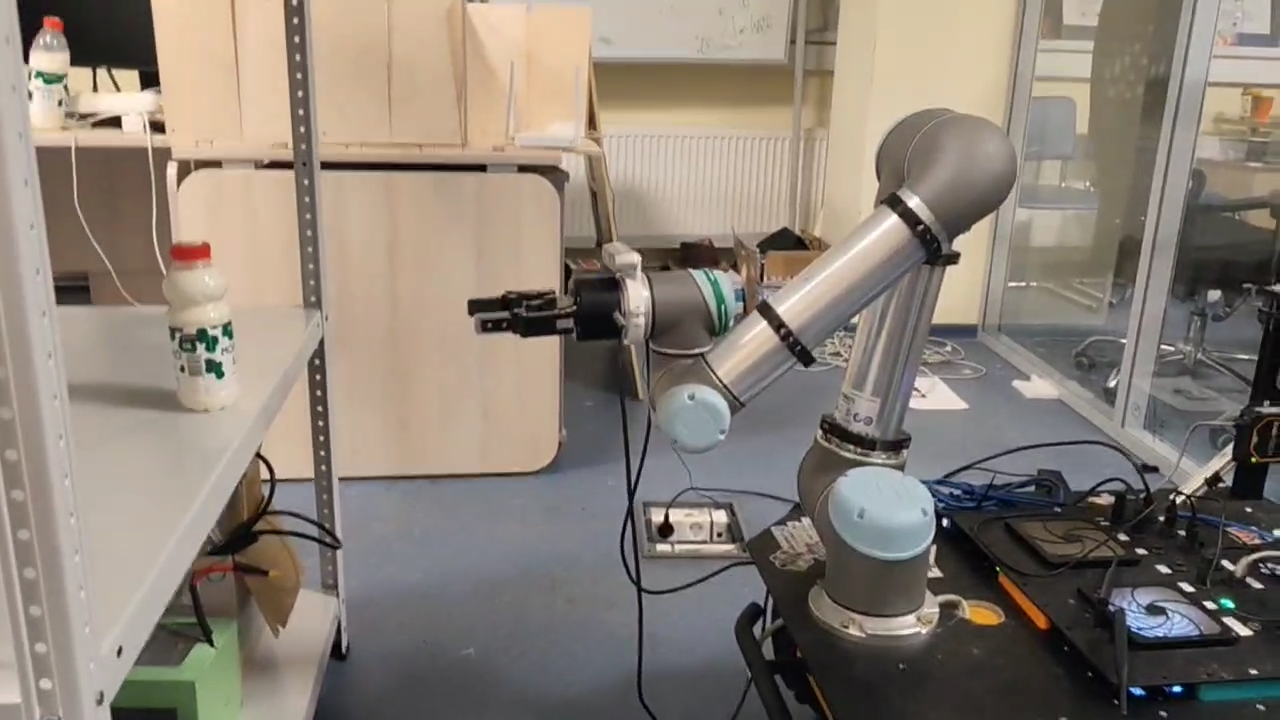
\includegraphics[height=6cm,width=1\textwidth,keepaspectratio]{video_2026-02-11_08-43-34.png}
            \label{fig:video_2026-02-11_08-43-34.png}
        \end{subfigure}

    \end{figure}
\end{frame}

\begin{frame}[t]{Pretest (1/2)}
    \framesubtitle{Robots, motion, and coordinate frames}
    \large

    \begin{enumerate}
        \item What distinguishes a robot from a conventional automated machine?

        \item What are the main components of a robotic system?

        \item What is a degree of freedom? How many degrees of freedom does a
        free rigid body have in 3D space?

        \item Do the coordinates of a physical point change when we choose a
        different coordinate frame?
    \end{enumerate}
\end{frame}

\begin{frame}[t]{Pretest (2/2)}
    \framesubtitle{Position, orientation, and pose}
    \large

    \begin{enumerate}
        \setcounter{enumi}{4}

        \item What is the difference between the position and orientation
        of an object?

        \item What methods can be used to represent the orientation of an
        object in 3D space?

        \item How can we represent both the position and orientation of an
        object relative to a coordinate frame?
    \end{enumerate}
\end{frame}

\begin{frame}[t]{Pretest Discussion (1/2)}
    \framesubtitle{Core ideas}

    \begin{itemize}
        \item \textbf{Robot}: A system that senses its environment, processes
        information, and acts on the physical world.

        \item \textbf{Main components}: Sensors, controller or computer,
        actuators, mechanical structure, and power supply.

        \item \textbf{Degree of freedom}: An independent variable required to
        describe motion.

        \item \textbf{Free rigid body in 3D}: Six degrees of freedom:
        three translations and three rotations.
    \end{itemize}
\end{frame}

\begin{frame}[t]{Pretest Discussion (2/2)}
    \framesubtitle{Position, orientation, and pose}

    \begin{itemize}
        \item \textbf{Position}: Location of an object, commonly represented by
        a vector
        \[
            \mathbf{p} =
            \begin{bmatrix}
                x & y & z
            \end{bmatrix}^{T}.
        \]

        \item \textbf{Orientation}: Angular relationship between two coordinate
        frames. Common representations include Euler or roll--pitch--yaw angles,
        rotation matrices, axis--angle, and quaternions.

        \item \textbf{Pose}: Position and orientation considered together.

        \item \textbf{Rotation order}: In general,
        \[
            \mathbf{R}_1\mathbf{R}_2
            \neq
            \mathbf{R}_2\mathbf{R}_1.
        \]
    \end{itemize}
\end{frame}

\begin{frame}[t]{Links and Joints}
    \framesubtitle{}
    \begin{columns}[T,onlytextwidth]
        \begin{column}{0.49\textwidth}
            \begin{figure}[H]
                \centering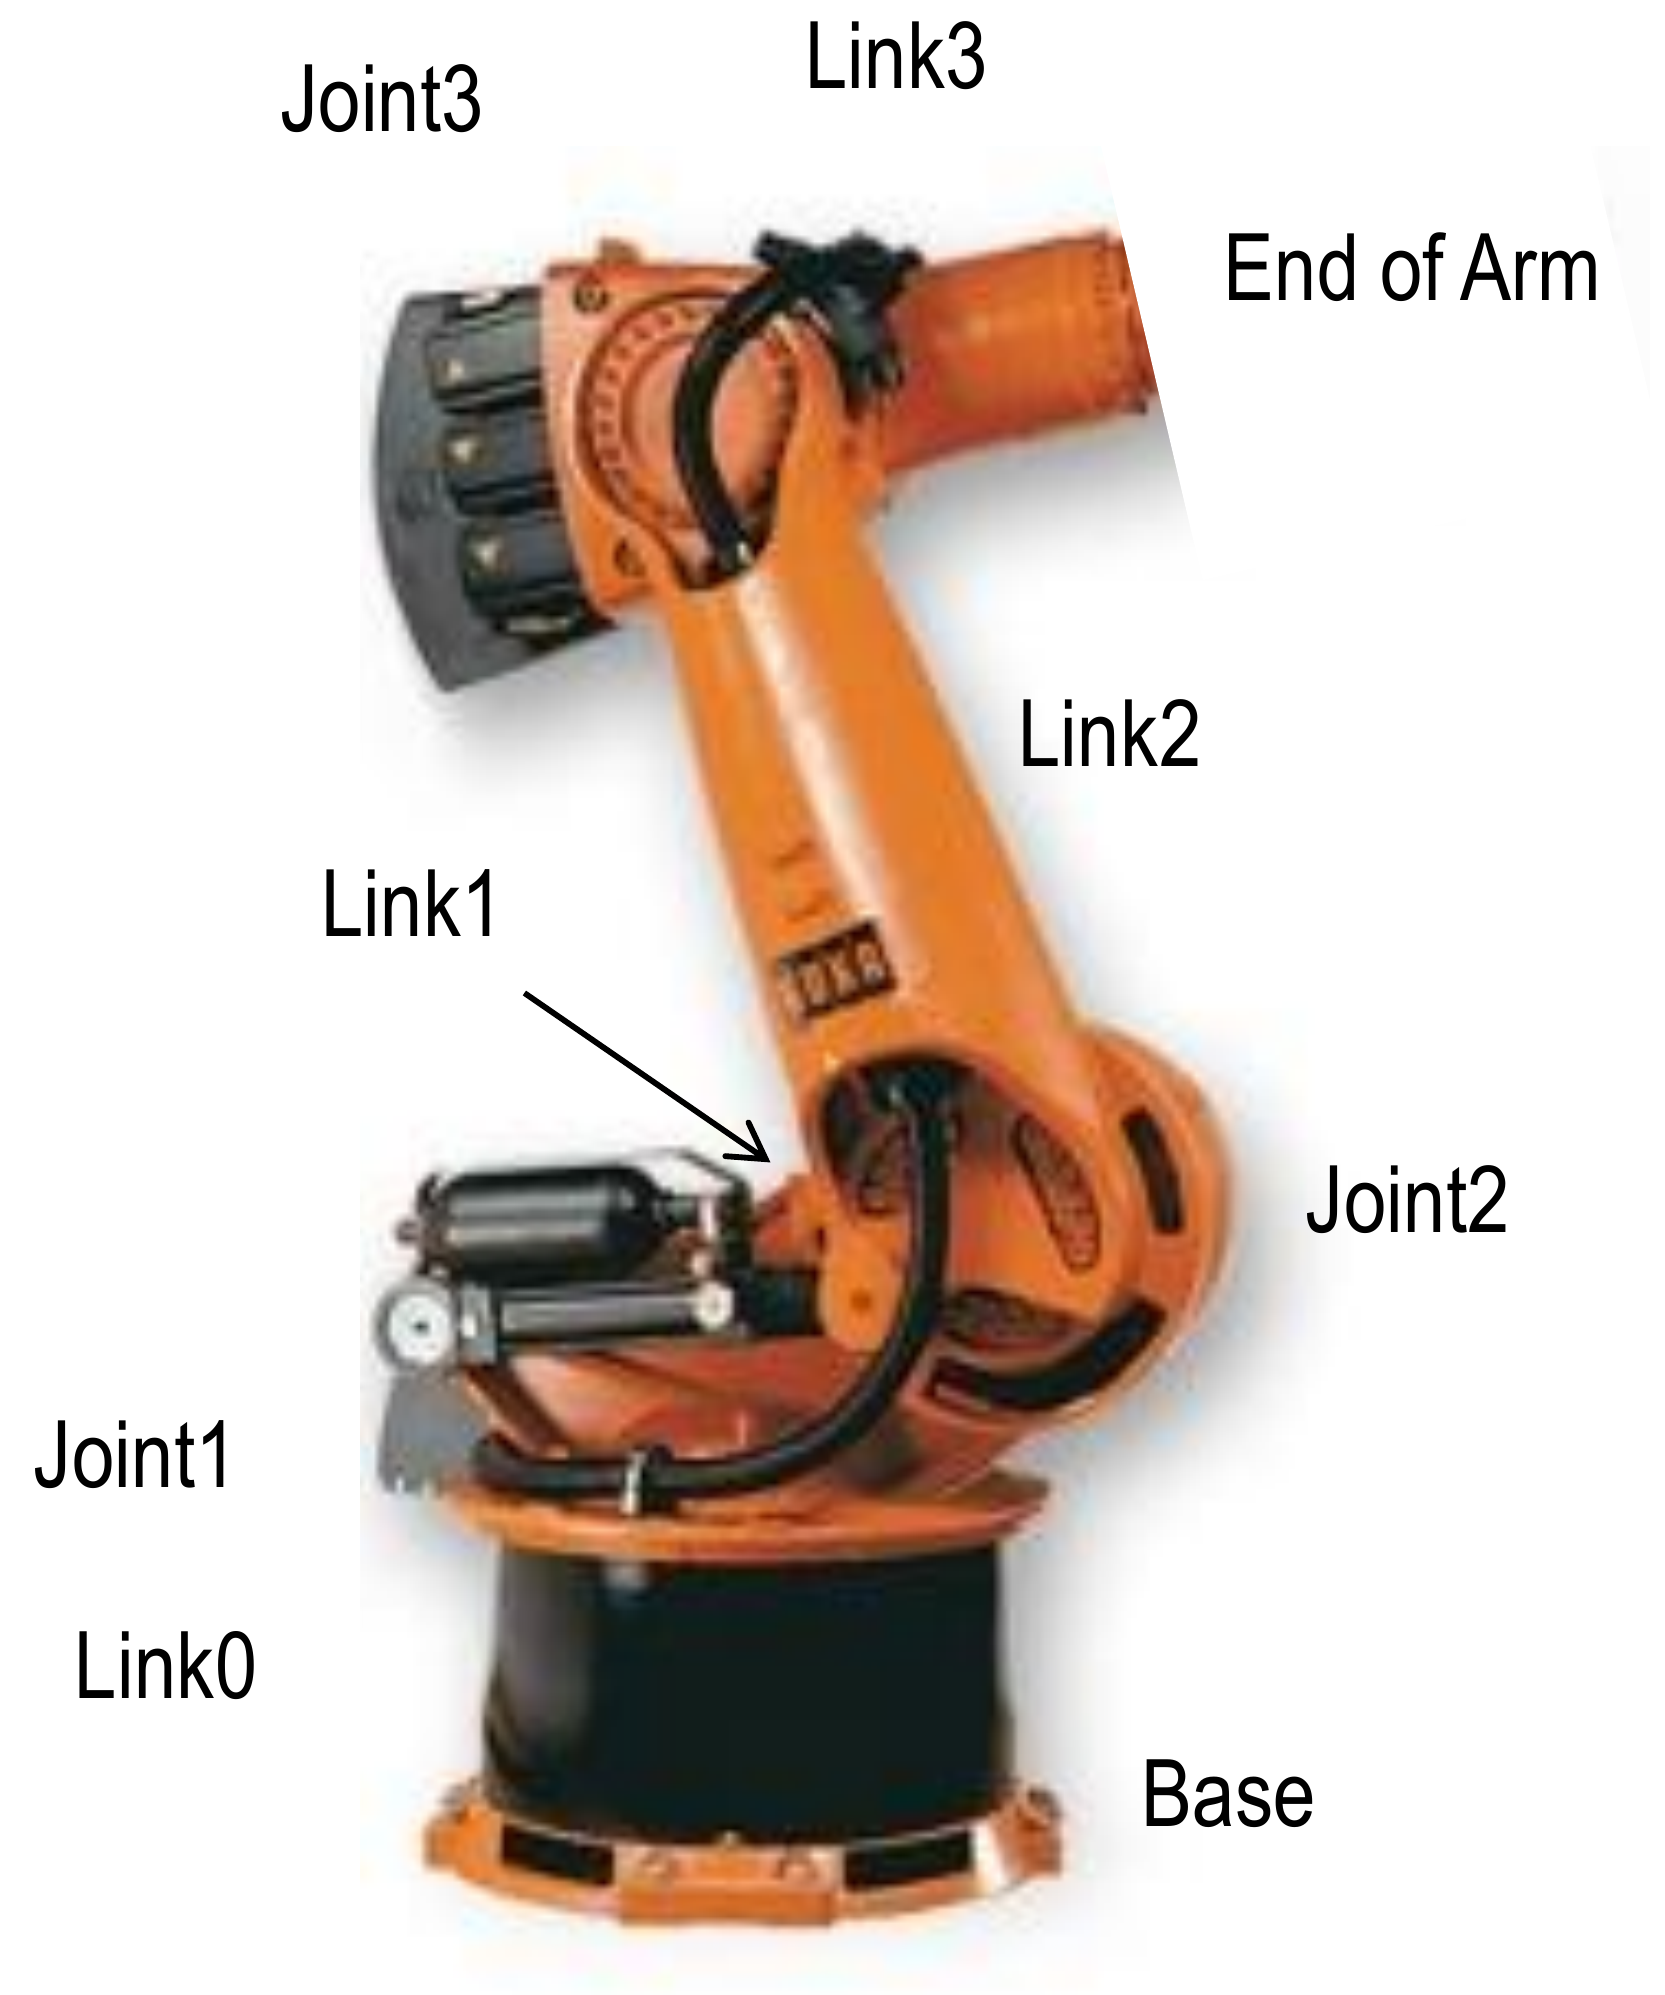
\includegraphics[height=5.5cm,width=\textwidth,keepaspectratio]{robot_anatomy/klimchik_p19_links_joints.png}
            \end{figure}
        \end{column}
        \begin{column}{0.49\textwidth}
            A manipulator consists of \textbf{links} and \textbf{joints}.
            \begin{itemize}
                \item \textbf{Links}: Rigid members between joints.
                \item \textbf{Joints}: Connections that provide relative motion between links.
            \end{itemize}
            \medskip
            A robot manipulator has two sections:
            \begin{itemize}
                \item \textbf{Body and arm}: Positioning objects in the robot's work volume.
                \item \textbf{Wrist}: Orienting objects.
            \end{itemize}
        \end{column}
    \end{columns}
\end{frame}

\begin{frame}[t]{Prismatic and Revolute Joints}
    \framesubtitle{}
    \begin{columns}[T,onlytextwidth]
        \begin{column}{0.39\textwidth}
            \begin{figure}[H]
                \centering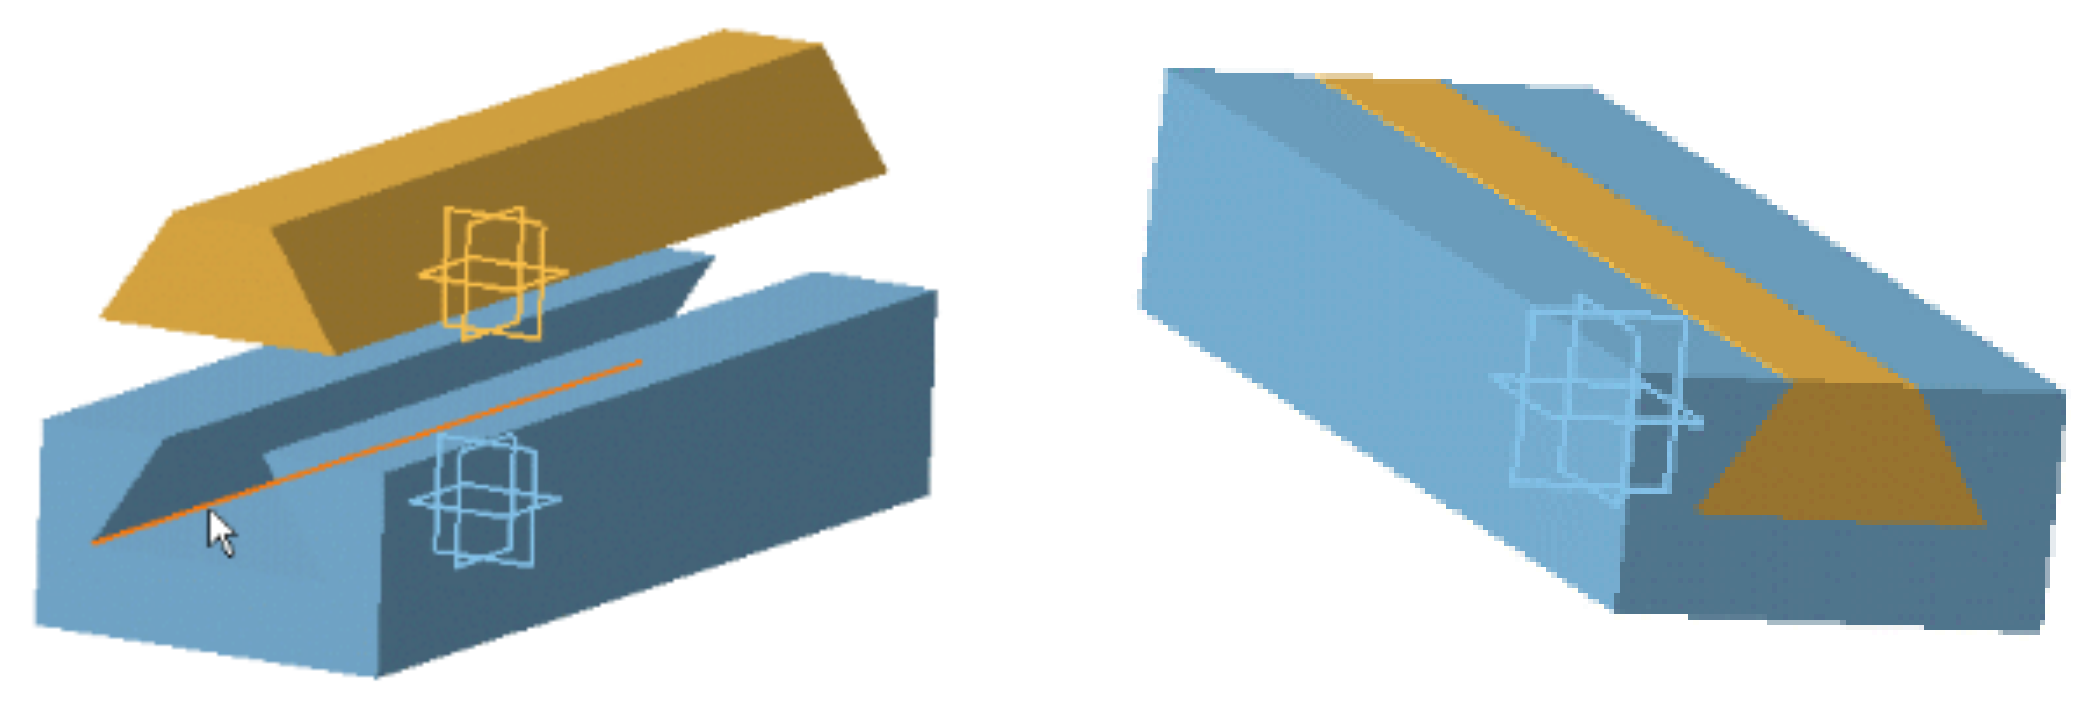
\includegraphics[height=2.2cm,width=\textwidth,keepaspectratio]{robot_anatomy/klimchik_p11_prismatic.png}
            \end{figure}
        \end{column}
        \begin{column}{0.59\textwidth}
            \textbf{Prismatic Joint (P)}
            \begin{itemize}
                \item Linear motion; no rotation.
                \item Actuation examples: hydraulic or pneumatic cylinder.
            \end{itemize}
        \end{column}
    \end{columns}
    \medskip
    \begin{columns}[T,onlytextwidth]
        \begin{column}{0.39\textwidth}
            \begin{figure}[H]
                \centering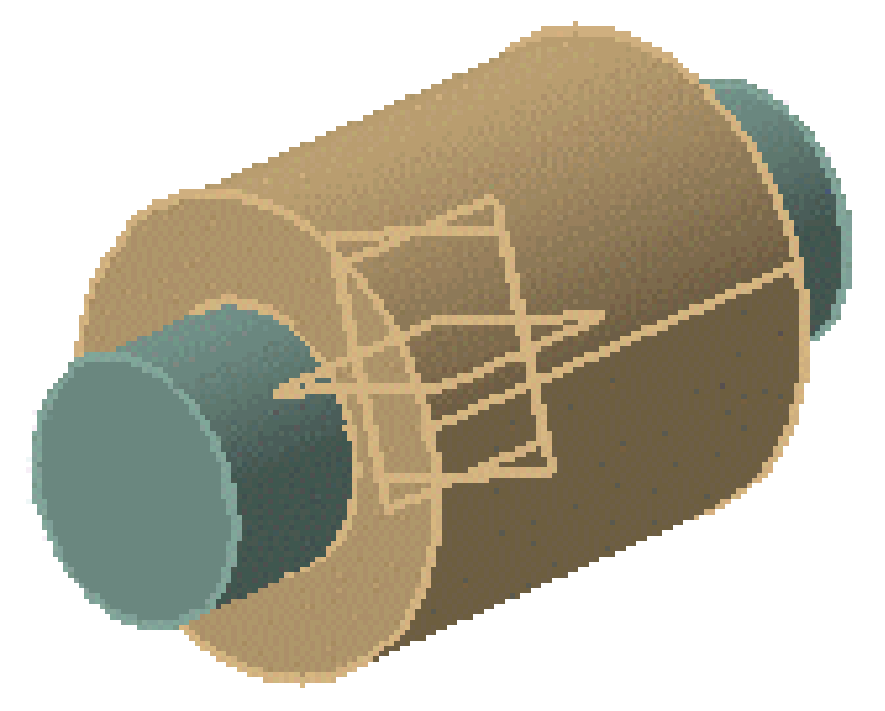
\includegraphics[height=2.2cm,width=\textwidth,keepaspectratio]{robot_anatomy/klimchik_p11_revolute.png}
            \end{figure}
        \end{column}
        \begin{column}{0.59\textwidth}
            \textbf{Revolute Joint (R)}
            \begin{itemize}
                \item Rotary motion.
                \item Actuation examples: stepper motor or servo motor.
            \end{itemize}
        \end{column}
    \end{columns}
\end{frame}

\begin{frame}[t]{Robot Types (1/2)}
    \framesubtitle{Body-and-arm configurations}
    \vspace{-0.3cm}
    \begin{columns}[T,onlytextwidth]
        \begin{column}{0.29\textwidth}
            \centering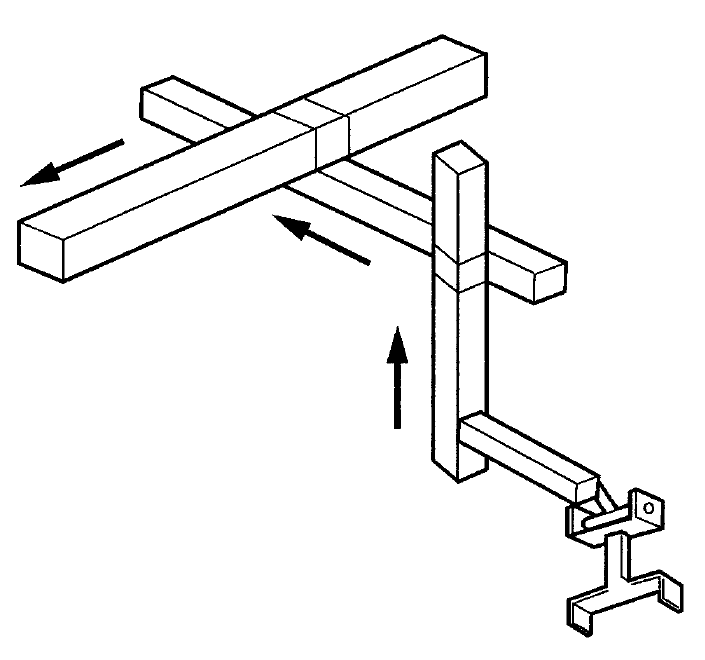
\includegraphics[height=1.65cm,width=\textwidth,keepaspectratio]{robot_anatomy/klimchik_p16_cartesian.png}
        \end{column}
        \begin{column}{0.69\textwidth}
            \textbf{Cartesian / Rectangular / Gantry (3P)}
            \begin{itemize}
                \item Three prismatic joints.
                \item Linear motion along the $X$, $Y$, and $Z$ axes.
            \end{itemize}
        \end{column}
    \end{columns}
    \medskip
    \begin{columns}[T,onlytextwidth]
        \begin{column}{0.29\textwidth}
            \centering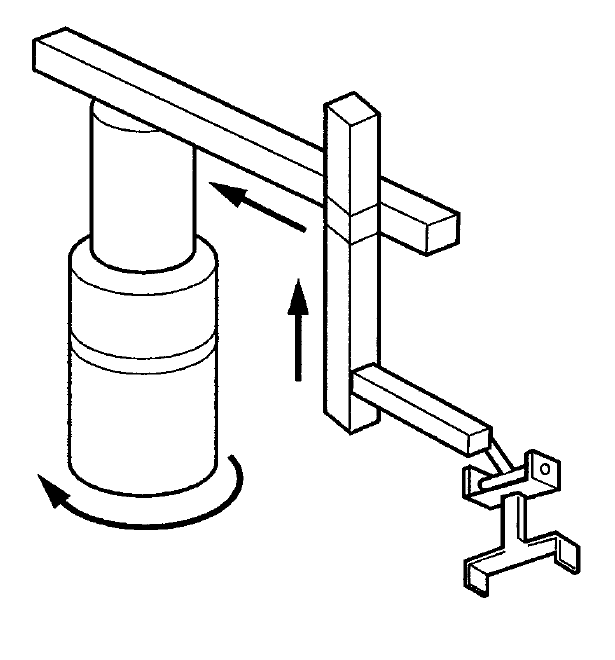
\includegraphics[height=1.65cm,width=\textwidth,keepaspectratio]{robot_anatomy/klimchik_p16_cylindrical.png}
        \end{column}
        \begin{column}{0.69\textwidth}
            \textbf{Cylindrical (R2P)}
            \begin{itemize}
                \item One revolute joint and two prismatic joints.
            \end{itemize}
        \end{column}
    \end{columns}
    \medskip
    \begin{columns}[T,onlytextwidth]
        \begin{column}{0.29\textwidth}
            \centering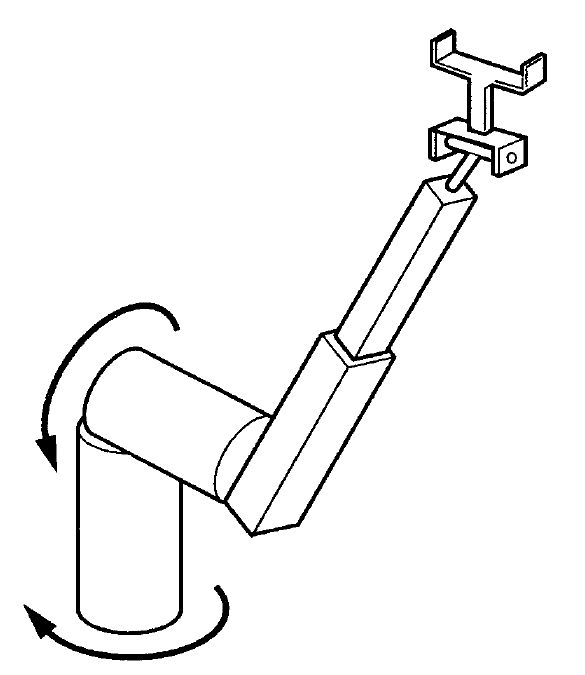
\includegraphics[height=1.65cm,width=\textwidth,keepaspectratio]{robot_anatomy/klimchik_p16_spherical.png}
        \end{column}
        \begin{column}{0.69\textwidth}
            \textbf{Spherical / Polar (2RP)}
            \begin{itemize}
                \item Two revolute joints and one prismatic joint.
            \end{itemize}
        \end{column}
    \end{columns}
\end{frame}

\begin{frame}[t]{Robot Types (2/2)}
    \framesubtitle{Body-and-arm configurations}
    \begin{columns}[T,onlytextwidth]
        \begin{column}{0.39\textwidth}
            \centering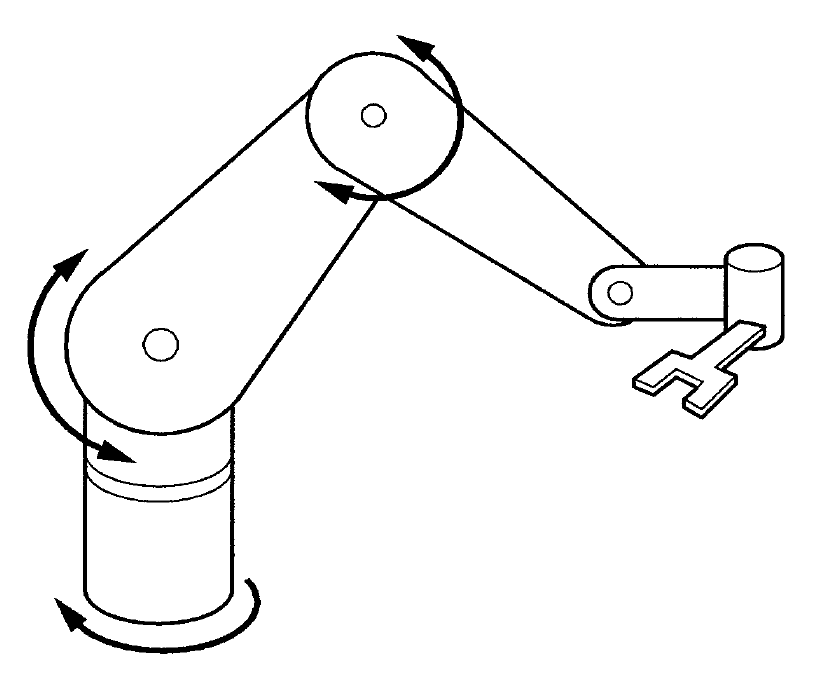
\includegraphics[height=2.3cm,width=\textwidth,keepaspectratio]{robot_anatomy/klimchik_p16_articulated.png}
        \end{column}
        \begin{column}{0.59\textwidth}
            \textbf{Articulated / Anthropomorphic (3R)}
            \begin{itemize}
                \item Three revolute joints.
                \item Human-arm-like configuration.
            \end{itemize}
        \end{column}
    \end{columns}
    \bigskip
    \begin{columns}[T,onlytextwidth]
        \begin{column}{0.39\textwidth}
            \centering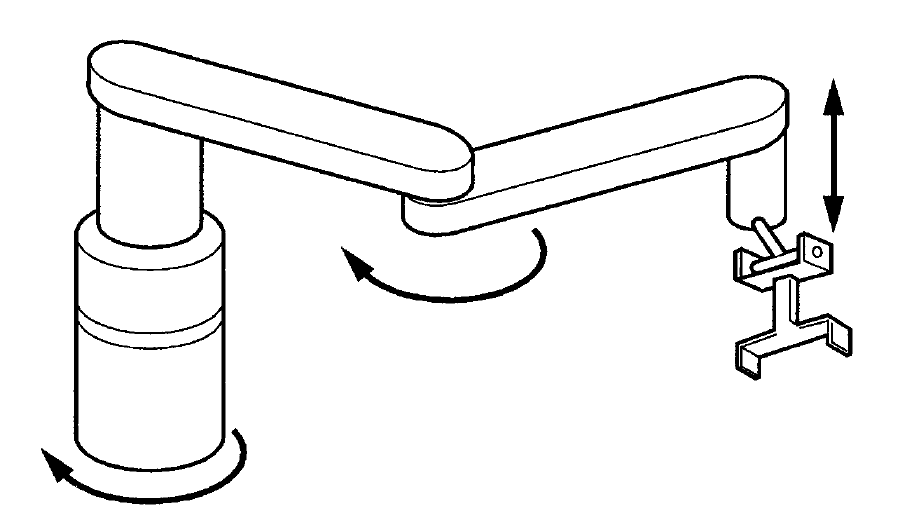
\includegraphics[height=2.3cm,width=\textwidth,keepaspectratio]{robot_anatomy/klimchik_p16_scara.png}
        \end{column}
        \begin{column}{0.59\textwidth}
            \textbf{SCARA}
            \begin{itemize}
                \item Selective Compliance Assembly Robot Arm.
                \item Illustrated positioning assembly: two revolute joints with parallel axes and one prismatic joint.
            \end{itemize}
        \end{column}
    \end{columns}
\end{frame}


\begin{frame}[t]{How Many Coordinates Describe a Rigid Body?}
    \begin{itemize}
        \item \textbf{In a plane: 3} --- two position coordinates and one orientation angle.
        \item \textbf{In space: 6} --- three position coordinates and three orientation parameters.
    \end{itemize}
    \begin{columns}[T,onlytextwidth]
        \begin{column}{0.49\textwidth}
            \centering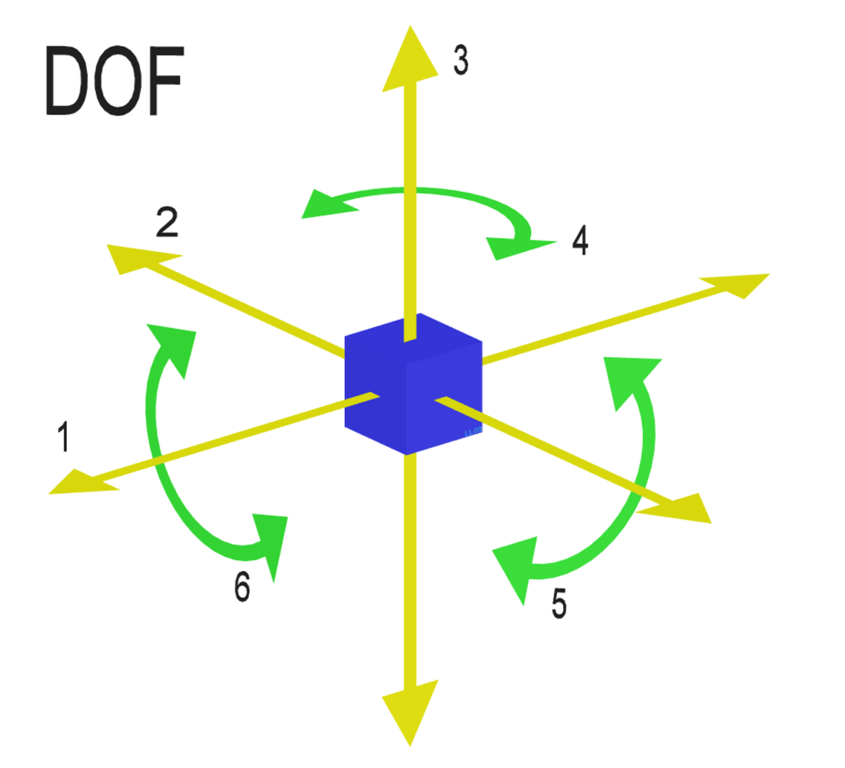
\includegraphics[height=3.5cm,width=\linewidth,keepaspectratio]{skillbox_la7/la7_image13.png}
        \end{column}
        \begin{column}{0.49\textwidth}
            \centering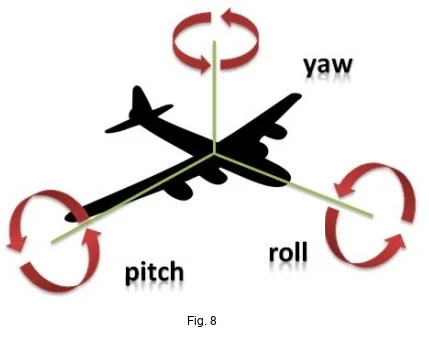
\includegraphics[height=3.5cm,width=\linewidth,keepaspectratio]{skillbox_la7/la7_image10.png}
        \end{column}
    \end{columns}
\end{frame}
\begin{frame}[t]{Position Representations}
    \begin{columns}[T,onlytextwidth]
        \begin{column}{0.35\textwidth}
            \textbf{2D}
            \begin{itemize}\item Cartesian\item Polar\end{itemize}
            \medskip\textbf{3D}
            \begin{itemize}\item Cartesian\item Cylindrical\item Spherical\end{itemize}
        \end{column}
        \begin{column}{0.63\textwidth}
            \centering
            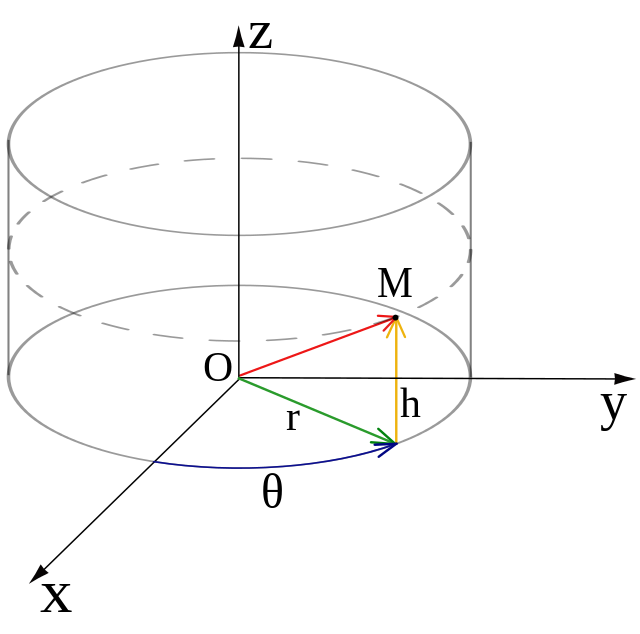
\includegraphics[height=2.35cm,width=.47\linewidth,keepaspectratio]{skillbox_la7/la7_image16.png}\hfill
            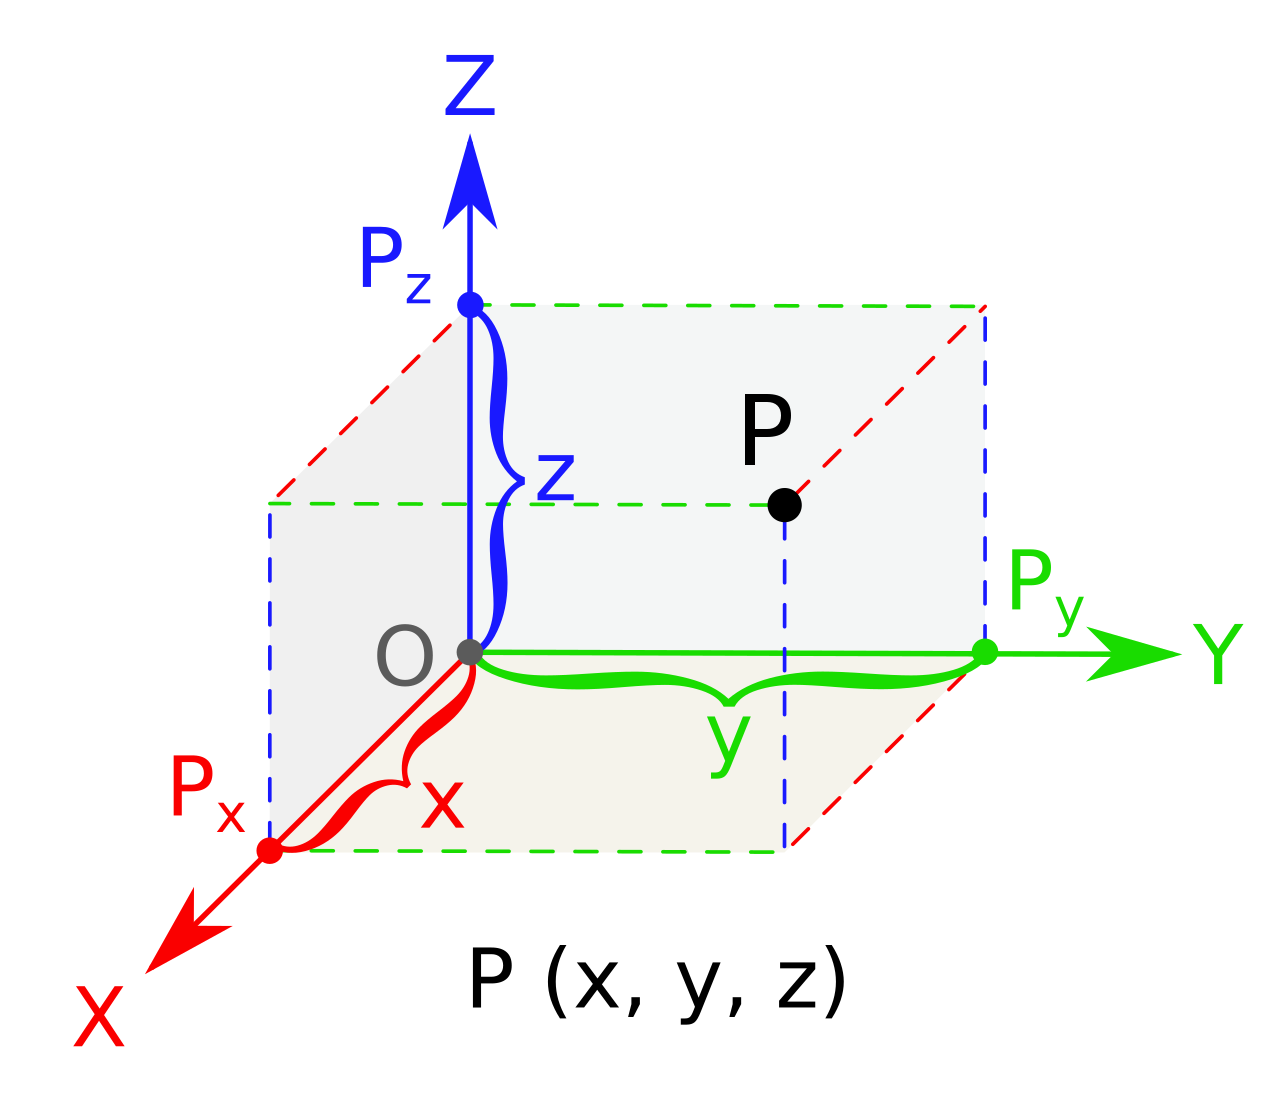
\includegraphics[height=2.35cm,width=.47\linewidth,keepaspectratio]{skillbox_la7/la7_image12.png}\\[0.2cm]
            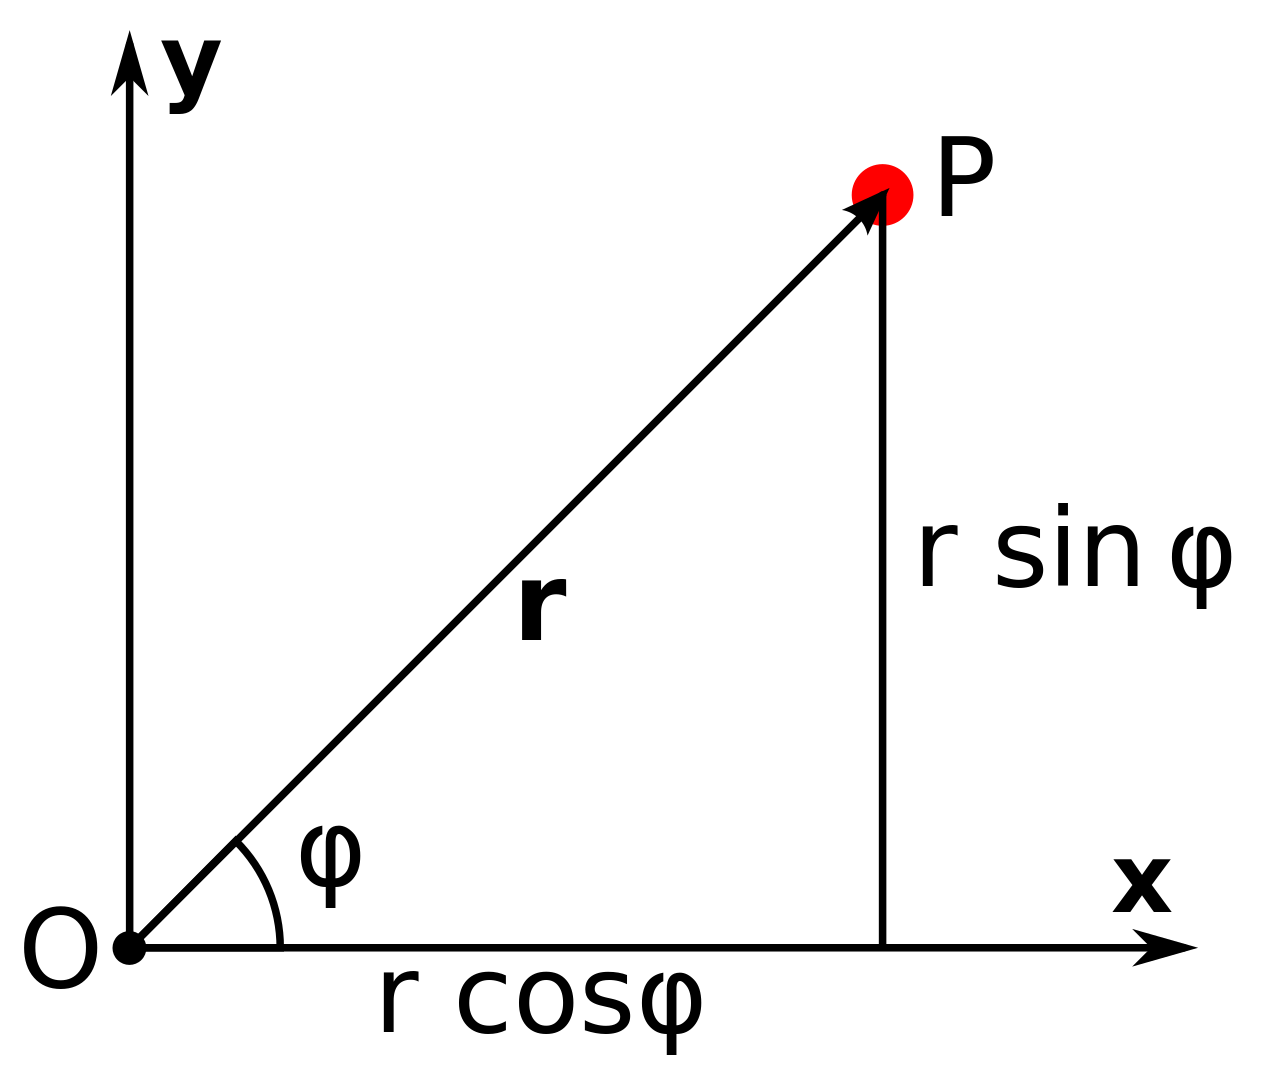
\includegraphics[height=2.35cm,width=.47\linewidth,keepaspectratio]{skillbox_la7/la7_image06.png}\hfill
            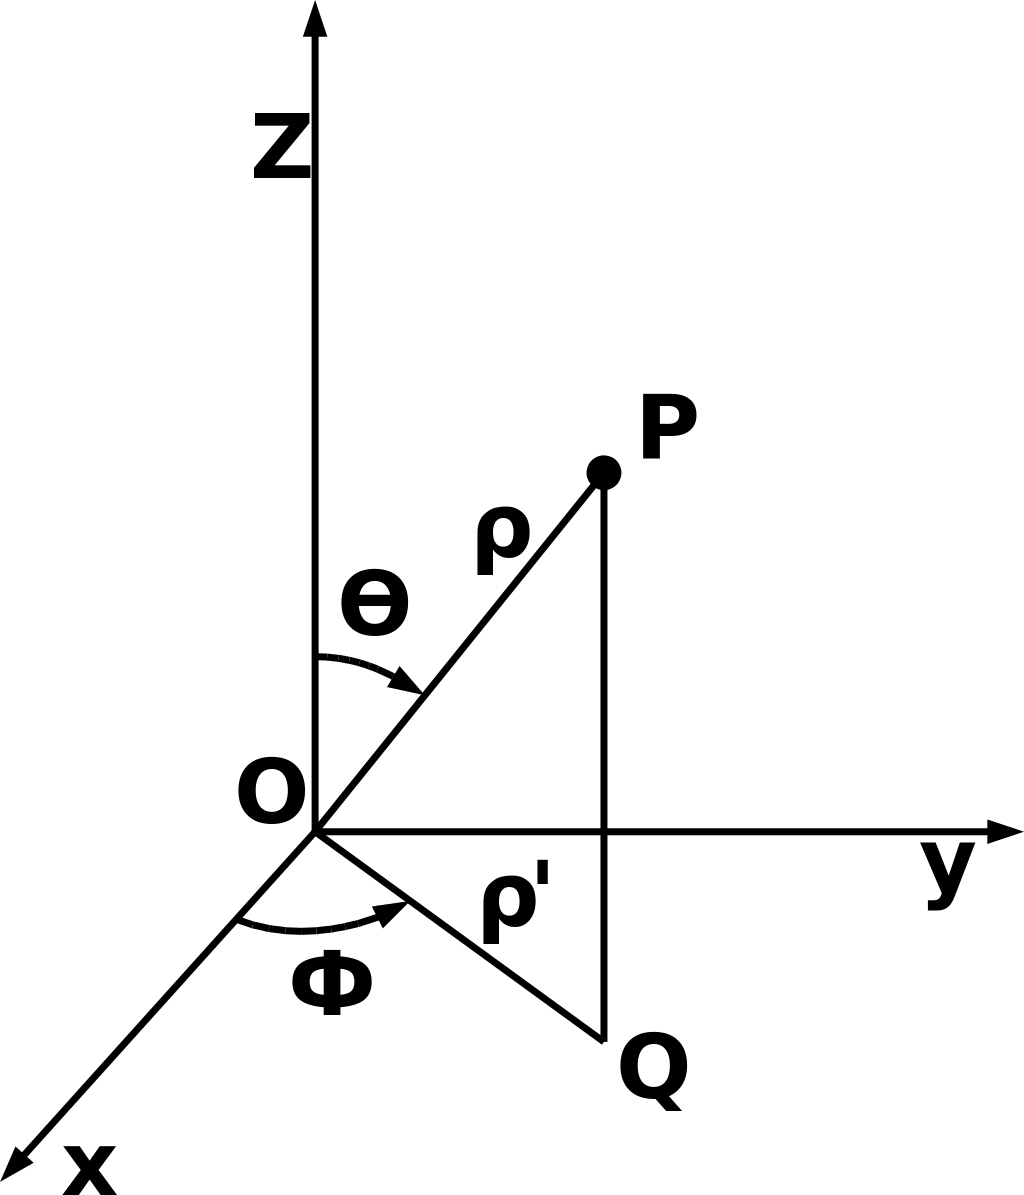
\includegraphics[height=2.35cm,width=.47\linewidth,keepaspectratio]{skillbox_la7/la7_image07.png}
        \end{column}
    \end{columns}
\end{frame}
\begin{frame}[t]{Orientation Representations}
    \begin{tabular}{@{}m{0.43\textwidth}m{0.53\textwidth}@{}}
        Rotation matrix: 9 parameters.
        & $\displaystyle R=\begin{bmatrix}r_{11}&r_{12}&r_{13}\\r_{21}&r_{22}&r_{23}\\r_{31}&r_{32}&r_{33}\end{bmatrix}$\\[0.2cm]
        & $\displaystyle \phantom{R}=\begin{bmatrix}\mathbf r_1&\mathbf r_2&\mathbf r_3\end{bmatrix}$\\[0.35cm]
        Euler angles: 3 parameters.
        & $(\alpha,\beta,\gamma)$\\[0.35cm]
        Axis-angle: 4 parameters.
        & $\displaystyle\left(\begin{bmatrix}e_x\\e_y\\e_z\end{bmatrix},\theta\right)
        =\left(\begin{bmatrix}0\\0\\-1\end{bmatrix},-\frac{\pi}{2}\right)$\\[0.35cm]
        Quaternion: 4 parameters.
        & $(x,y,z,w)$
    \end{tabular}
\end{frame}
\begin{frame}[t]{Rotation Matrices}
    \only<1>{
        $R\in SO(n)$, the \textbf{special orthogonal group} of $n\times n$ matrices.
        The columns form an orthonormal basis:
        \[R^TR=I,\qquad R^T=R^{-1},\qquad \det R=1.\]
        \medskip
        Elementary rotations in 3D, with $c=\cos\varphi$, $s=\sin\varphi$:
        \begin{align*}
            R_x(\varphi)&=\begin{bmatrix}1&0&0\\0&c&-s\\0&s&c\end{bmatrix},&
            R_y(\varphi)&=\begin{bmatrix}c&0&s\\0&1&0\\-s&0&c\end{bmatrix},\\
            R_z(\varphi)&=\begin{bmatrix}c&-s&0\\s&c&0\\0&0&1\end{bmatrix}.
        \end{align*}
    }
    \only<2>{
        A sequence of rotations has an explicitly specified order:
        \[R=R_x(\alpha)R_y(\beta)R_z(\gamma).\]
        With $c_a=\cos\alpha$, $s_a=\sin\alpha$ (and similarly for $b,c$):
        \small
        \[R=\begin{bmatrix}1&0&0\\0&c_a&-s_a\\0&s_a&c_a\end{bmatrix}
        \begin{bmatrix}c_b&0&s_b\\0&1&0\\-s_b&0&c_b\end{bmatrix}
        \begin{bmatrix}c_c&-s_c&0\\s_c&c_c&0\\0&0&1\end{bmatrix}\]
        \medskip
        \[=\begin{bmatrix}
            c_bc_c&-c_bs_c&s_b\\
            s_as_bc_c+c_as_c&-s_as_bs_c+c_ac_c&-s_ac_b\\
            s_as_c-c_as_bc_c&s_ac_c+c_as_bs_c&c_ac_b
        \end{bmatrix}.\]
    }
\end{frame}
\begin{frame}[t]{Euler Angles}
    Rotate about $z$, then the \textbf{new} $y$, then the \textbf{newest} $z$ axis.
    \[R_{ZYZ}=R_z(\phi)R_y(\theta)R_z(\psi).\]
    \small
    \[R_{ZYZ}=\begin{bmatrix}
        c_\phi c_\theta c_\psi-s_\phi s_\psi&-c_\phi c_\theta s_\psi-s_\phi c_\psi&c_\phi s_\theta\\
        s_\phi c_\theta c_\psi+c_\phi s_\psi&-s_\phi c_\theta s_\psi+c_\phi c_\psi&s_\phi s_\theta\\
        -s_\theta c_\psi&s_\theta s_\psi&c_\theta
    \end{bmatrix}\]
    \centering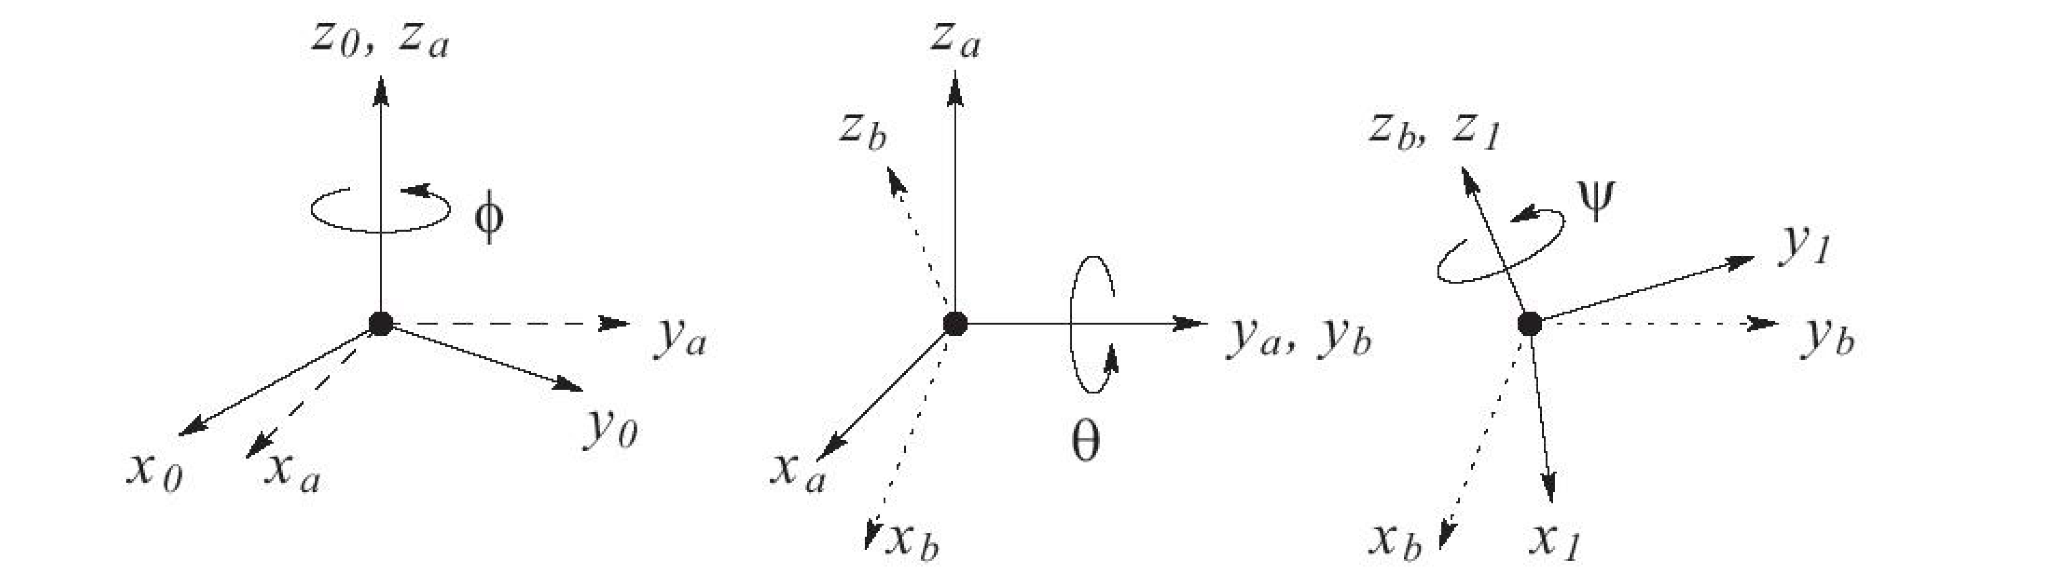
\includegraphics[height=2.0cm,width=.86\textwidth,keepaspectratio]{skillbox_la7/la7_euler_axes.png}
    \par\normalsize\medskip
    \textbf{Problem: gimbal lock.}\quad $c_\eta=\cos\eta$, $s_\eta=\sin\eta$.
\end{frame}
\begin{frame}[t]{Fixed Angles}
    Three successive rotations about fixed principal axes:
    \textbf{roll} ($x$), \textbf{pitch} ($y$), \textbf{yaw} ($z$).
    \[R=R_z(\phi)R_y(\theta)R_x(\psi),\qquad c_\eta=\cos\eta,\ s_\eta=\sin\eta.\]
    \small
    \[R=\begin{bmatrix}
        c_\phi c_\theta&c_\phi s_\theta s_\psi-s_\phi c_\psi&c_\phi s_\theta c_\psi+s_\phi s_\psi\\
        s_\phi c_\theta&s_\phi s_\theta s_\psi+c_\phi c_\psi&s_\phi s_\theta c_\psi-c_\phi s_\psi\\
        -s_\theta&c_\theta s_\psi&c_\theta c_\psi
    \end{bmatrix}\]
    \begin{columns}[T,onlytextwidth]
        \begin{column}{0.39\textwidth}\centering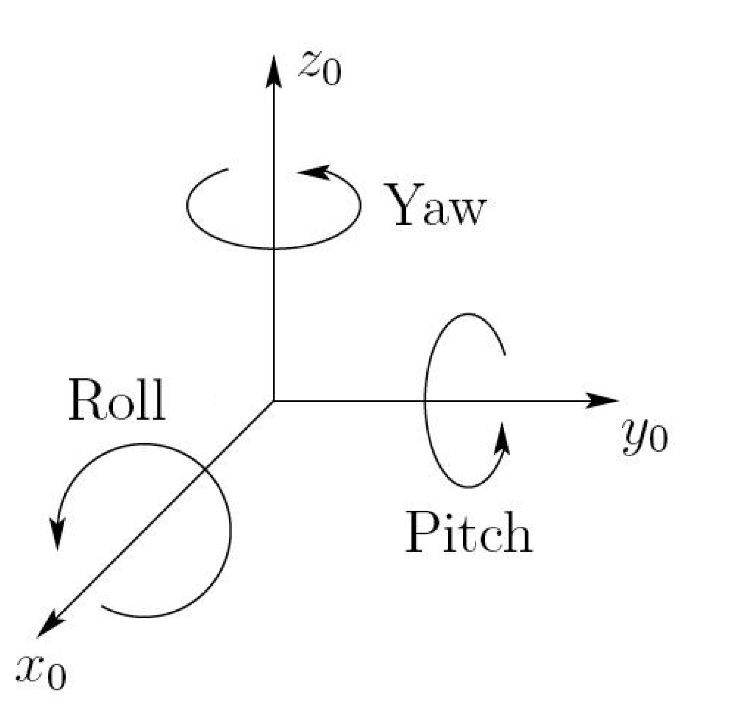
\includegraphics[height=2.1cm,width=\linewidth,keepaspectratio]{skillbox_la7/la7_fixed_axes.png}\end{column}
        \begin{column}{0.59\textwidth}\centering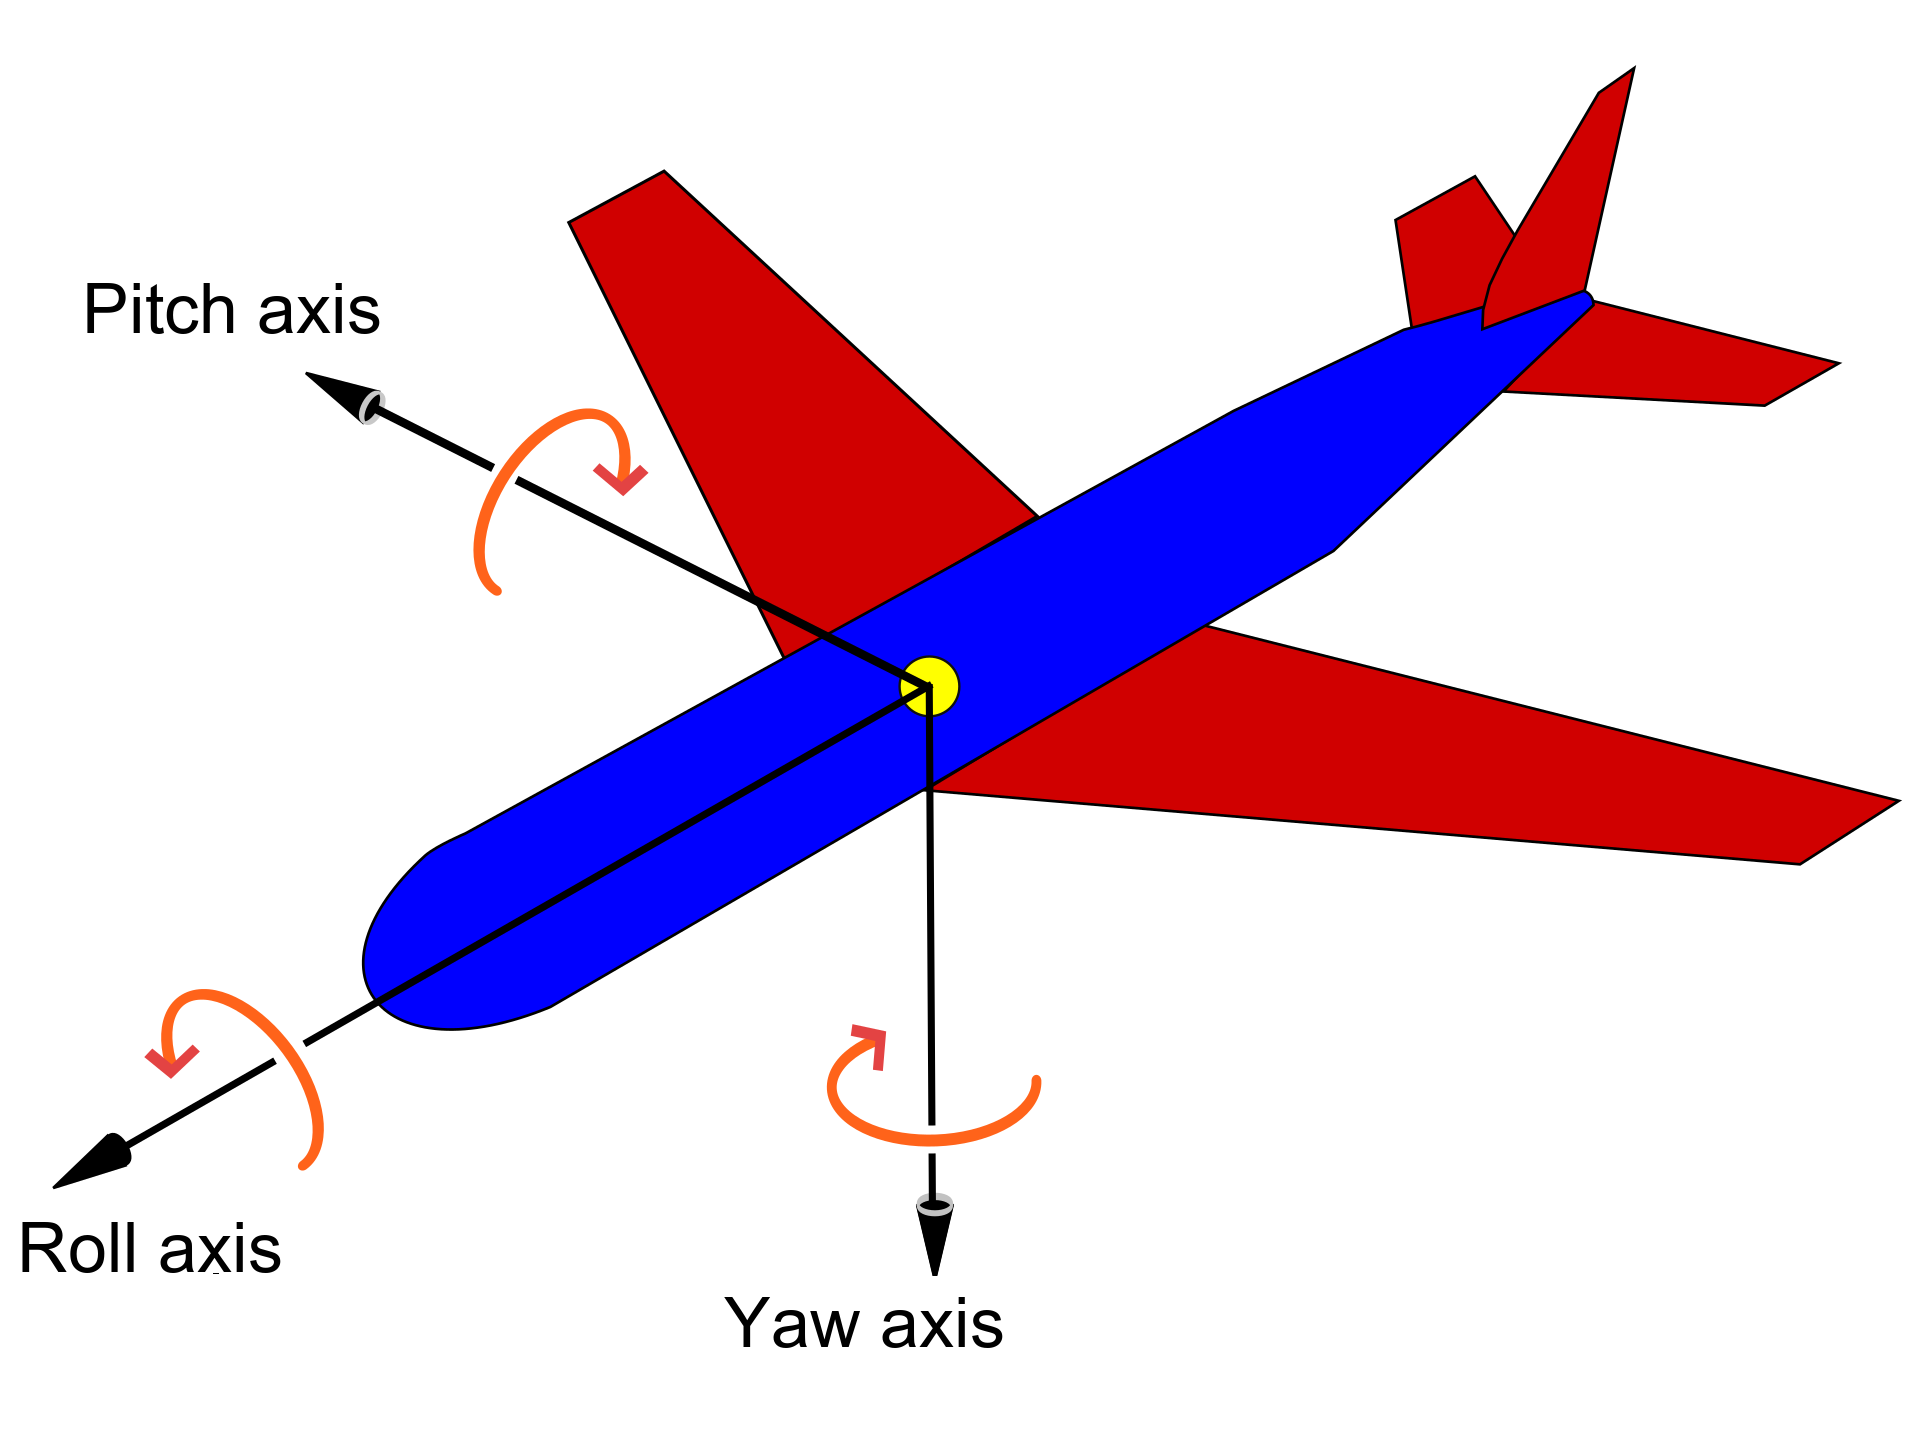
\includegraphics[height=2.1cm,width=\linewidth,keepaspectratio]{skillbox_la7/la7_image18.png}\end{column}
    \end{columns}
\end{frame}
\begin{frame}[t]{Axis-Angle}
    \begin{columns}[T,onlytextwidth]
        \begin{column}{0.64\textwidth}
            \[(\mathrm{axis},\mathrm{angle})=
            \left(\begin{bmatrix}e_x\\e_y\\e_z\end{bmatrix},\theta\right)
            =\left(\begin{bmatrix}0\\0\\-1\end{bmatrix},-\frac{\pi}{2}\right).\]
            \medskip
            Unit axis $\mathbf u=(u_x,u_y,u_z)^T$;\\
            $c=\cos\theta$, $s=\sin\theta$, $v=1-c$.
        \end{column}
        \begin{column}{0.34\textwidth}
            \centering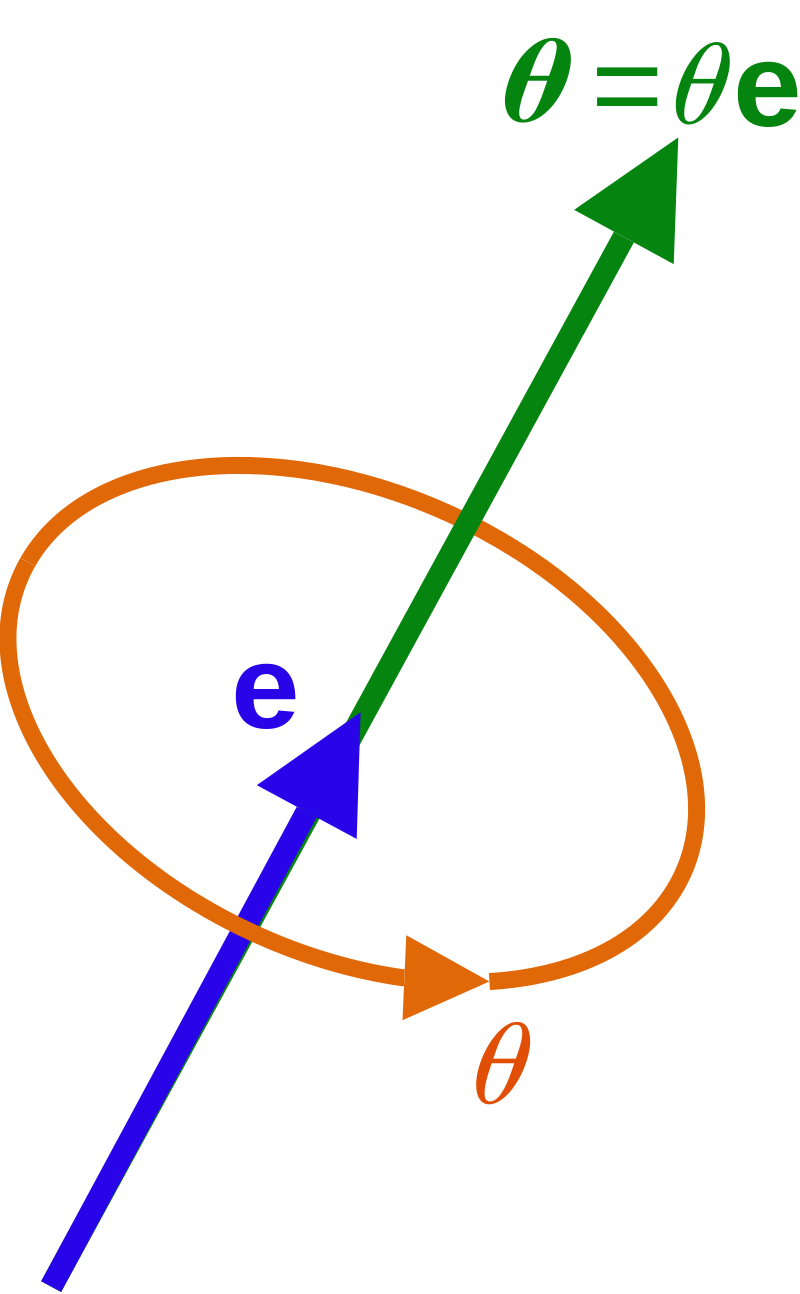
\includegraphics[height=2.7cm,width=\linewidth,keepaspectratio]{skillbox_la7/la7_image15.png}
        \end{column}
    \end{columns}
    \medskip
    \[R=\begin{bmatrix}
        c+u_x^2v&u_xu_yv-u_zs&u_xu_zv+u_ys\\
        u_yu_xv+u_zs&c+u_y^2v&u_yu_zv-u_xs\\
        u_zu_xv-u_ys&u_zu_yv+u_xs&c+u_z^2v
    \end{bmatrix}.\]
\end{frame}
\begin{frame}[t]{Quaternions}
    Quaternions provide a convenient mathematical representation of
    orientations and rotations in space.
    \medskip

    Compared with Euler angles, they make rotation composition convenient
    and avoid gimbal lock.
    \medskip

    \[q=q_r+q_i\mathbf i+q_j\mathbf j+q_k\mathbf k,\qquad s=\|q\|^{-2}.\]
    \small
    \[R=\begin{bmatrix}
        1-2s(q_j^2+q_k^2)&2s(q_iq_j-q_kq_r)&2s(q_iq_k+q_jq_r)\\
        2s(q_iq_j+q_kq_r)&1-2s(q_i^2+q_k^2)&2s(q_jq_k-q_iq_r)\\
        2s(q_iq_k-q_jq_r)&2s(q_jq_k+q_iq_r)&1-2s(q_i^2+q_j^2)
    \end{bmatrix}.\]
    \normalsize\medskip
    The four components parameterize $q$; for a unit quaternion, $s=1$.
\end{frame}


\begin{frame}[t]{Orientation Representations}
    \framesubtitle{Task 1}
    \only<1>{
        A coordinate frame rotates by $20^{\circ}$ about its $x$ axis,
        then by $45^{\circ}$ about its \textbf{new} $z$ axis,
        and finally by $70^{\circ}$ about its \textbf{new} $x$ axis.
        \medskip

        Express the resulting orientation as:
        \begin{enumerate}
            \item A rotation matrix.
            \item Euler angles.
            \item Fixed angles.
            \item A quaternion.
            \item An axis--angle pair.
        \end{enumerate}
    }
    \only<2>{
        \alert{\Large Answer}\medskip

        Moving-axis rotations give the intrinsic $XZX$ sequence:
        \[R=R_x(20^{\circ})R_z(45^{\circ})R_x(70^{\circ}).\]
        \[R\approx\begin{bmatrix}
        0.707107&-0.241845&0.664463\\
        0.664463&-0.094134&-0.741369\\
        0.241845&0.965738&0.094134
        \end{bmatrix}.\]
        \medskip
        \begin{itemize}
            \item \textbf{Euler angles (intrinsic $XZX$):} $(20^{\circ},45^{\circ},70^{\circ})$.
            \item \textbf{Fixed angles (extrinsic $xzx$):} $(70^{\circ},45^{\circ},20^{\circ})$.
        \end{itemize}
    }
    \only<3>{
        \alert{\Large Answer}\medskip

        Quaternion, with the scalar component first:
        \[q=q_x(20^{\circ})q_z(45^{\circ})q_x(70^{\circ})\]
        \[q\approx 0.653281+0.653281\mathbf i+0.161729\mathbf j+0.346829\mathbf k.\]
        \medskip
        \[\theta=2\arccos(q_r)\approx98.421058^{\circ},\qquad
        \mathbf u=\frac{(q_i,q_j,q_k)^T}{\sin(\theta/2)}.\]
        \[(\mathbf u,\theta)\approx
        \left(\begin{bmatrix}0.862856\\0.213612\\0.458093\end{bmatrix},98.421058^{\circ}\right).\]
    }
\end{frame}
\begin{frame}[t]{Summary}
    \begin{enumerate}
        \item A rigid-body pose requires \textbf{six coordinates in space}
        and \textbf{three in a plane}.
        \medskip
        \item We considered five position representations across 2D and 3D.
        \medskip
        \item We examined four orientation representations
        and how they relate to one another.
    \end{enumerate}
\end{frame}


\begin{frame}[t]{Changing Basis}
    \framesubtitle{Case Study: Shoe Polishing Robot}
    \vspace{-0.6cm}
    \begin{figure}[H]
        \centering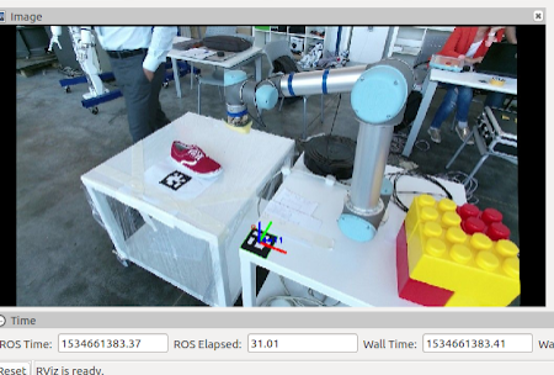
\includegraphics[height=6cm,width=1\textwidth,keepaspectratio]{change_basis_practice_2.png}
        \label{fig:change_basis_practice_2.png}
    \end{figure}
\end{frame}

\begin{frame}[t]{Changing Basis}
    \framesubtitle{Case Study: Shoe Polishing Robot, How it works}
    \vspace{-0.6cm}
    \begin{figure}[H]
        \centering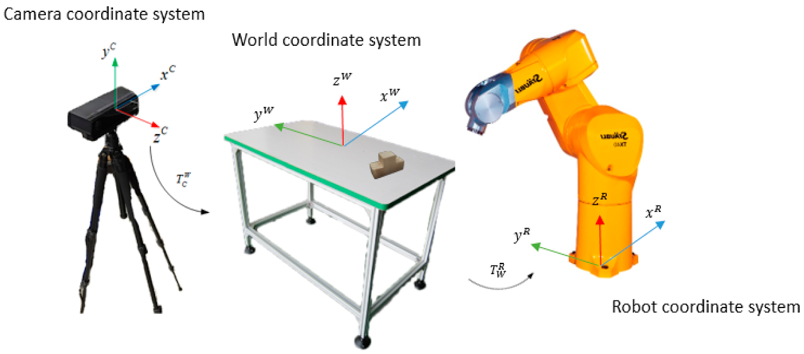
\includegraphics[height=6cm,width=1\textwidth,keepaspectratio]{change_basis_practice_1.png}
        \label{fig:change_basis_practice_1.png}
    \end{figure}
\end{frame}

\begin{frame}[t]{Changing Basis}
    \framesubtitle{Two Bros in the World of Changing Basis}
    \LARGE \centering$E' = EA$ and $Ex=E'x'$.

    Extended Bro Equation: $Ex = Eb + E'x'$, where $E = [e_1\ e_2\ e_3] = \begin{bmatrix}e_{1x}\\e_{1y} \\ e_{1z}\end{bmatrix},\ \begin{bmatrix}e_{2x}\\e_{2y} \\ e_{2z}\end{bmatrix},\ \begin{bmatrix}e_{3x}\\e_{3y} \\ e_{3z}\end{bmatrix}$, $E' = [e'_1\ e'_2\ e'_3]$ \smallskip
\end{frame}

\usebackgroundtemplate{}
\setbeamercolor{background canvas}{bg=}
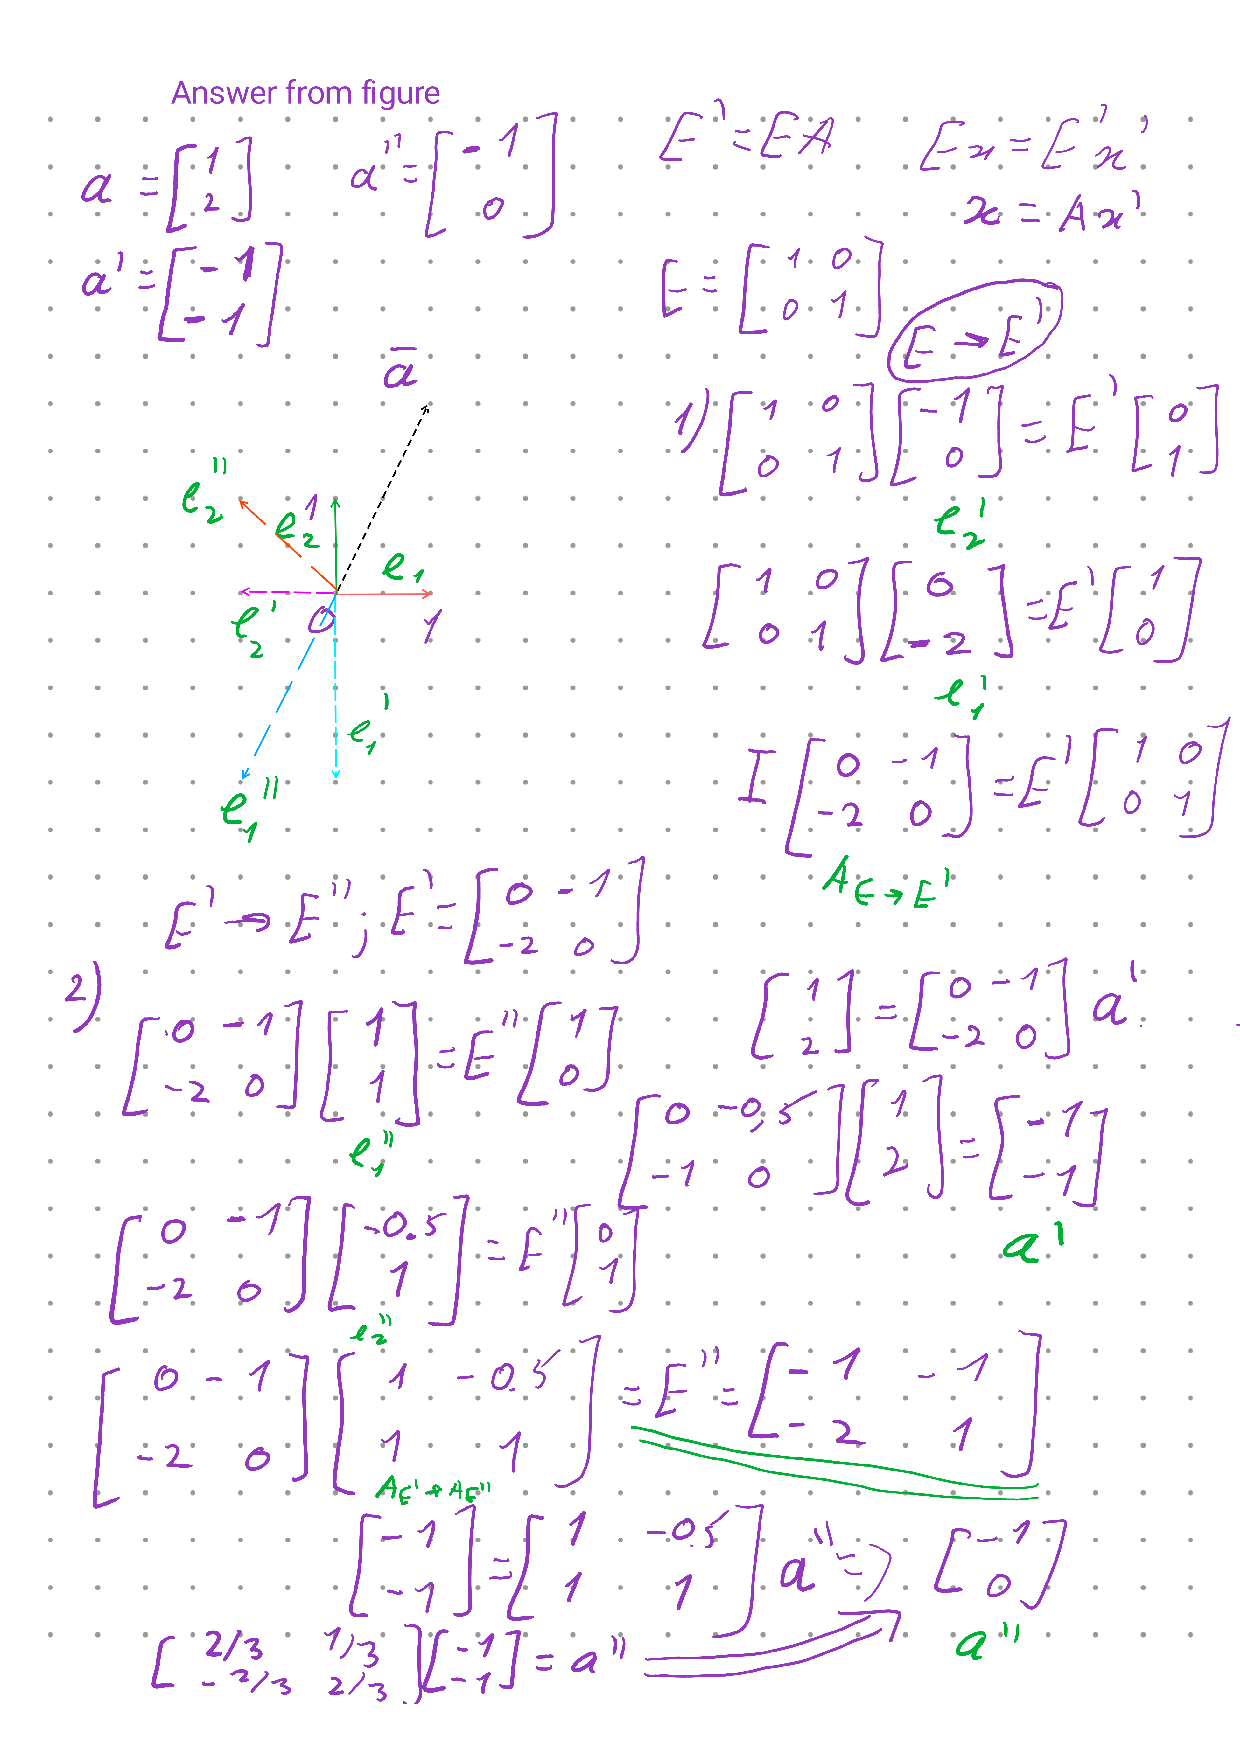
\includepdf[pages=-,fitpaper, linktodoc=true, pagecommand={\section{two_bros}\label{pdf:two_bros}}]{two_bros_fig.pdf}
\fbckg{fibeamer/figs/common.png}

\begin{frame}[t]{Changing Basis}
    \framesubtitle{Task 2}
    \only<1>{If vectors \textbf{a} and \textbf{b} form a basis (you should check it), it is needed to find coordinates $\textbf{c}$ in the basis.\medskip

    $\textbf{a}=\begin{bmatrix} -5 \\ -1 \end{bmatrix}$, $\textbf{b}=\begin{bmatrix} -1 \\ 3\end{bmatrix}$,
    $\textbf{c}=\begin{bmatrix} -1 \\ 2 \end{bmatrix}$.}
    \only<2>{\alert{\Large Answer}

    \begin{align*}
        E = \begin{bmatrix}
        1 & 0\\ 
        0 & 1 
        \end{bmatrix},\ E' = \begin{bmatrix}
        -5 & -1\\ 
        -1 & 3 
        \end{bmatrix} \\
        \text{Because we are interested in coordinates, 2nd bro} \\
        Ec_{old} = E'x \rightarrow \begin{bmatrix}
            1 & 0\\ 
            0 & 1 
            \end{bmatrix}\begin{bmatrix} -1\\ 2 \end{bmatrix} = \begin{bmatrix}
            -5 & -1\\ 
            -1 & 3 
            \end{bmatrix}\begin{bmatrix} c_{new_x}\\c_{new_y} \end{bmatrix} \\
            \begin{bmatrix} c_{new_x}\\c_{new_y} \end{bmatrix} = (E')^{-1}c_{old} = \begin{bmatrix} \frac{1}{16}\\ \frac{11}{16} \end{bmatrix}
    \end{align*}
    }
    \only<3>{
        \vspace{-0.6cm}
        \begin{figure}[H]
            \href{https://www.geogebra.org/calculator/zyamrfcn}{
                \centering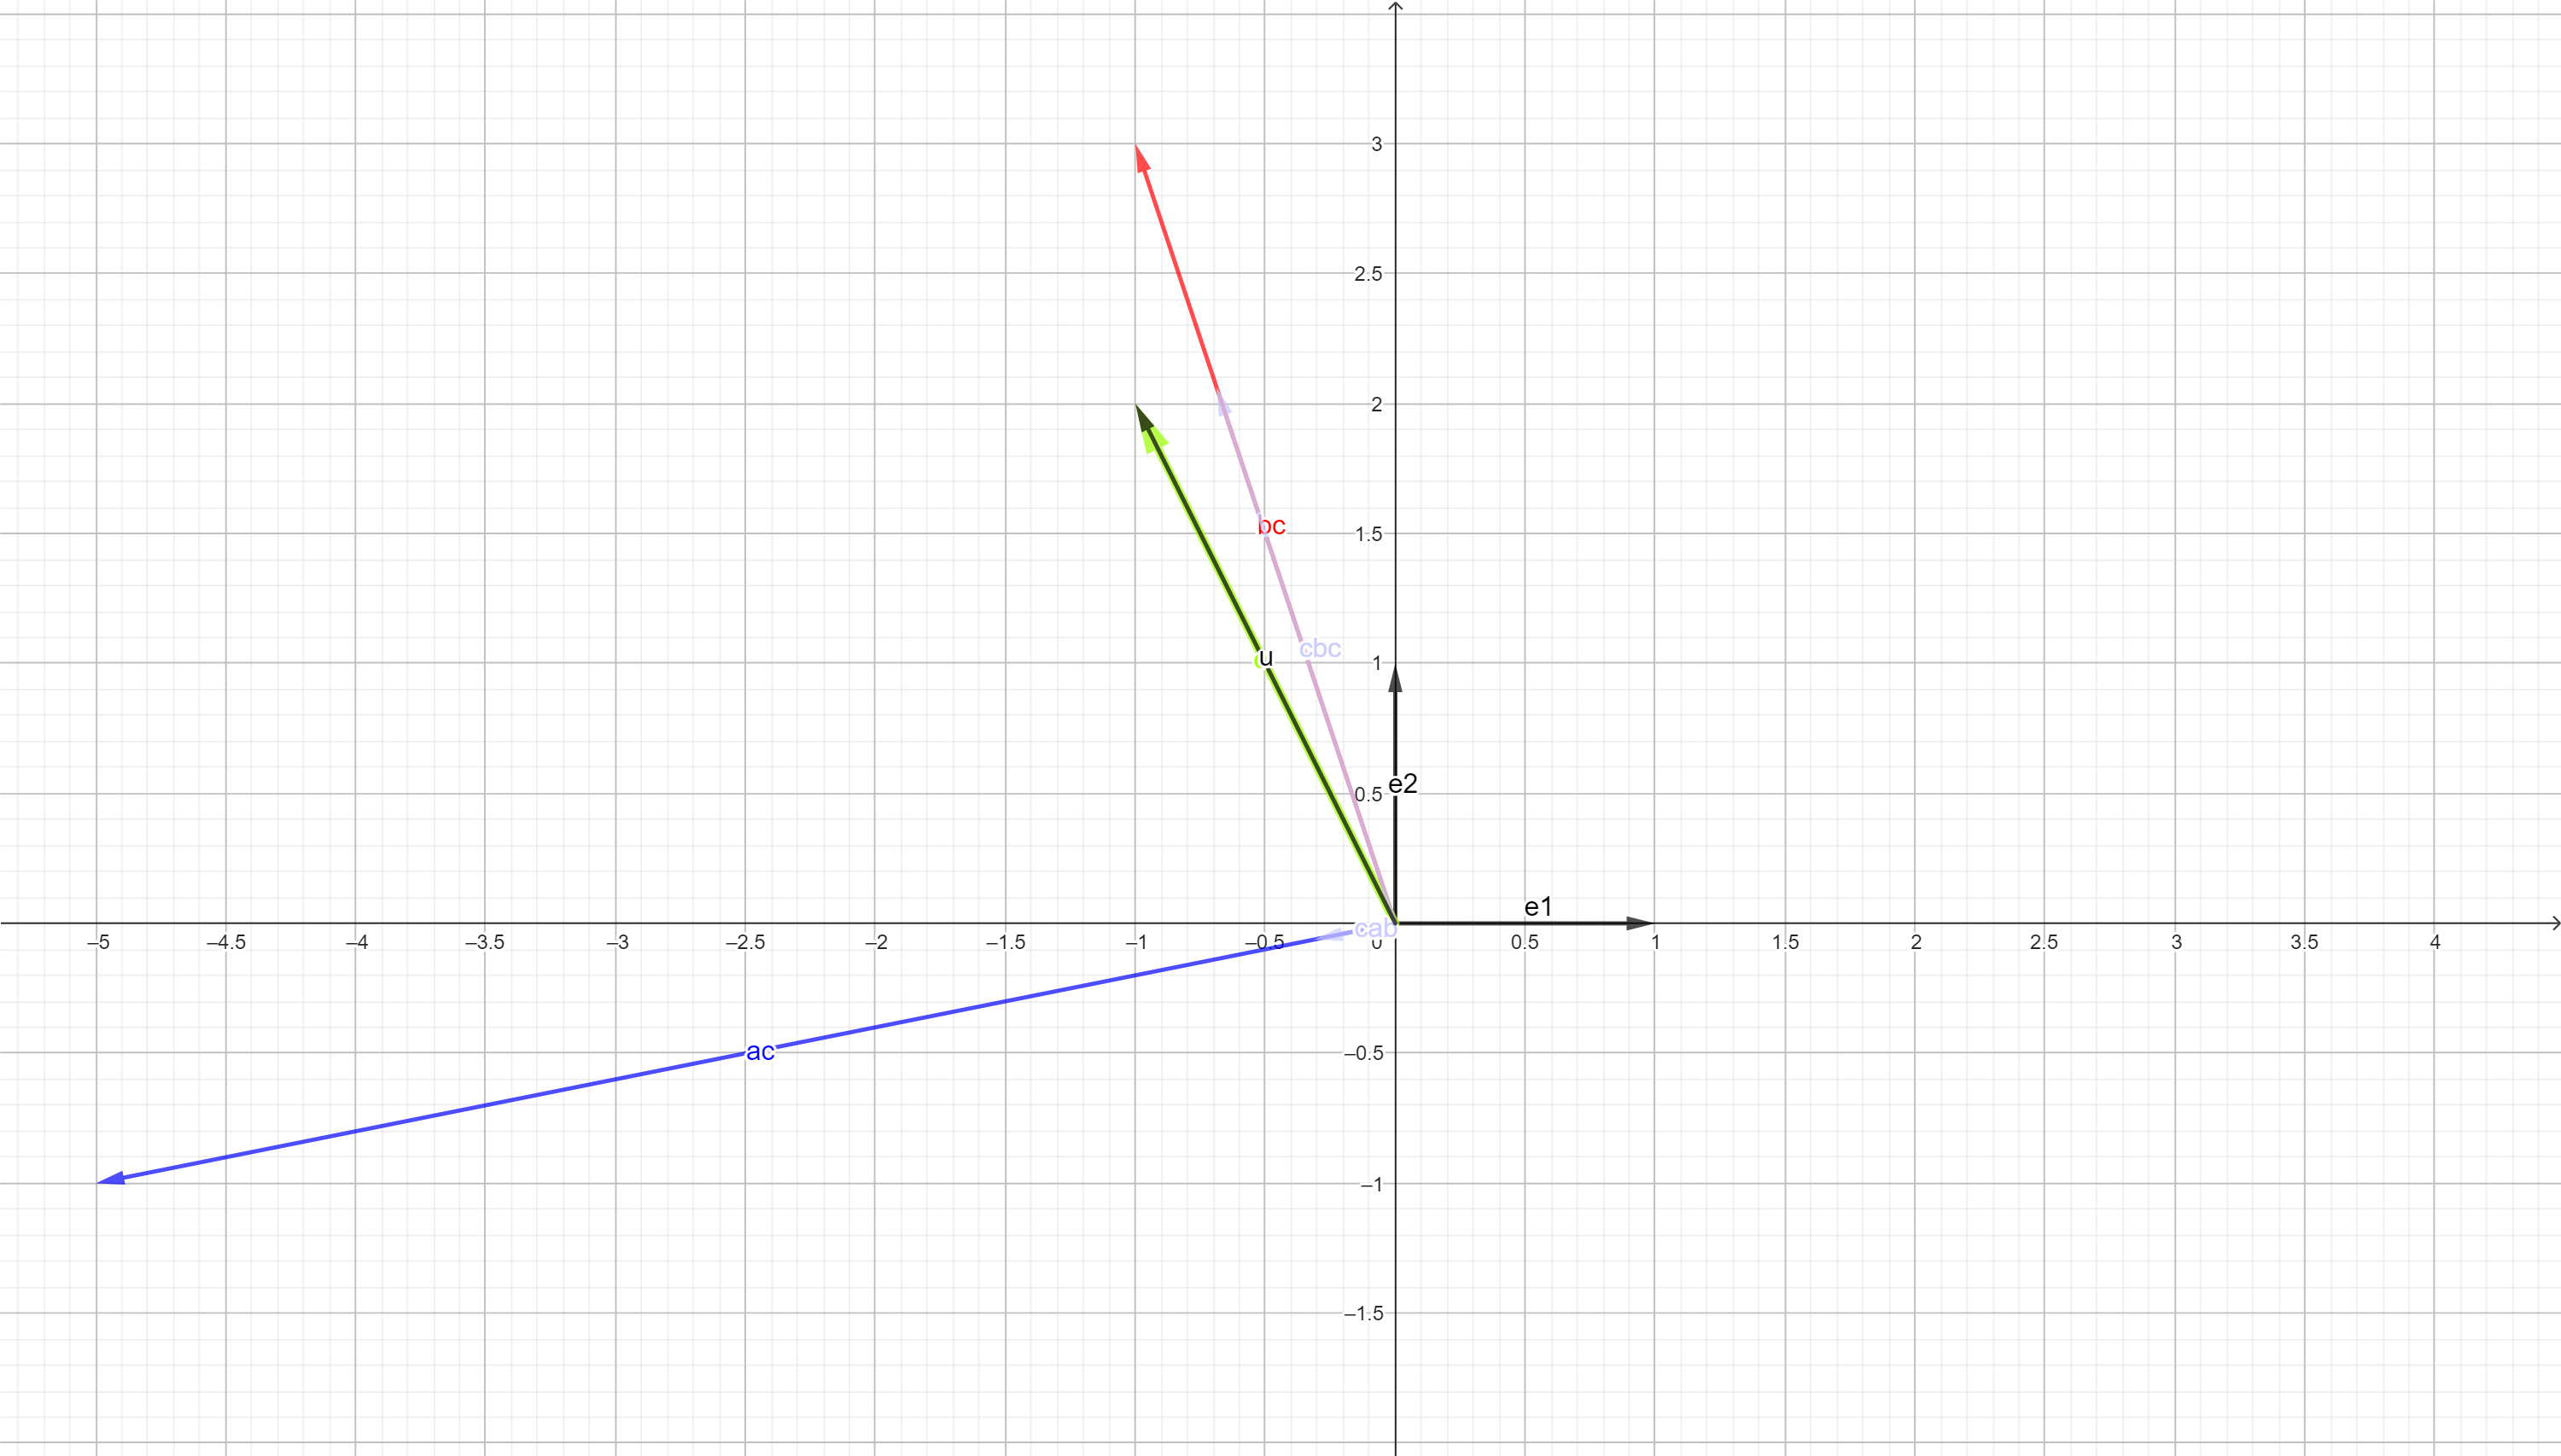
\includegraphics[height=6cm,width=1\textwidth,keepaspectratio]{resources/lab4_t3.png}}
            \label{fig:resources/lab4_t3.png}
        \end{figure}
    }
\end{frame}




\begin{frame}[t]{Changing Basis}
    \framesubtitle{Homogeneous representation}
    \vspace{-0.6cm}
    \begin{figure}[H]
        \centering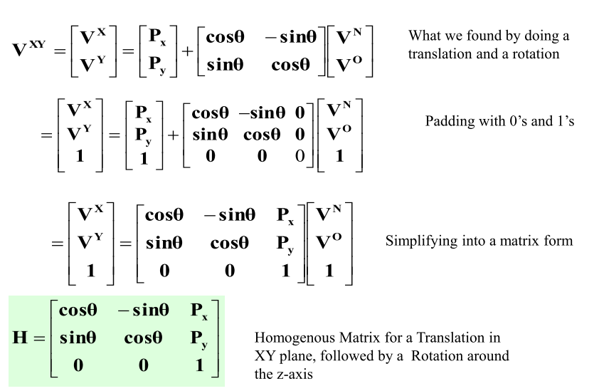
\includegraphics[height=6cm,width=1\textwidth,keepaspectratio]{change_klimchik_2.png}
        \label{fig:change_klimchik_2.png}
    \end{figure}
\end{frame}

\begin{frame}[t]{Changing Basis}
    \framesubtitle{Special Cases of Homogeneous matrices in 3D}
    \vspace{-0.6cm}
    \begin{figure}[H]
        \centering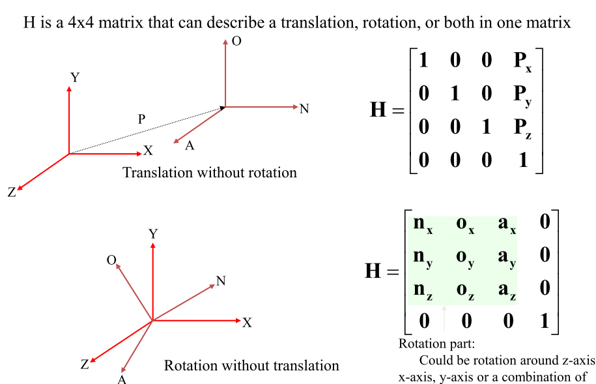
\includegraphics[height=6cm,width=1\textwidth,keepaspectratio]{change_klimchik_3.png}
        \label{fig:change_klimchik_3.png}
    \end{figure}
\end{frame}

\begin{frame}[t]{Changing Basis}
    \framesubtitle{Change the coordinate frame: Case Study}
    \vspace{-0.6cm}
    \begin{figure}[H]
        \centering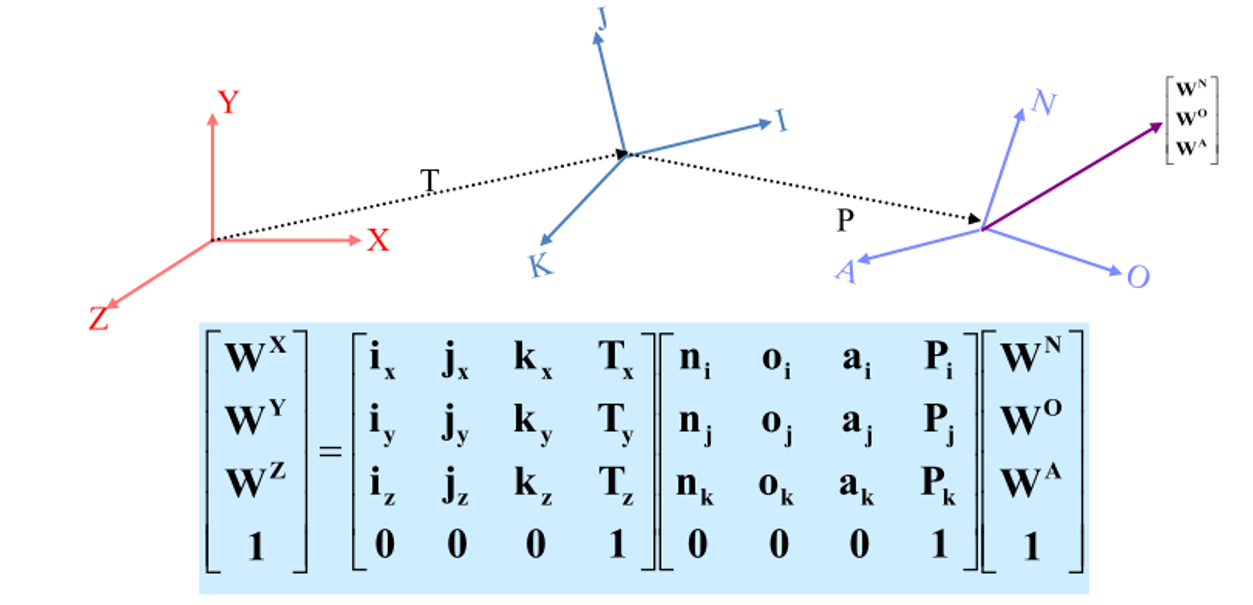
\includegraphics[height=6cm,width=1\textwidth,keepaspectratio]{change_klimchik_4.png}
        \label{fig:change_klimchik_4.png}
    \end{figure}
\end{frame}

\begin{frame}[t]{Changing Basis}
    \framesubtitle{Task 3}
    \only<1>{
    Let us consider two coordinate systems in the plane: $O$, $\textbf{e}_1$, $\textbf{e}_2$ and $O'$, $\textbf{e}'_1$, $\textbf{e}'_2$. Point $O'$ has coordinates $(7;-2)$ in the old coordinate system, and vectors $\textbf{e}'_1$, $\textbf{e}'_2$ can be obtained from vectors $\textbf{e}_1$, $\textbf{e}_2$ by rotating them $60^{\circ}$ (a) clockwise; (b) counterclockwise. Find the old coordinates of a point $x$, $y$ given its new coordinates $x'$, $y'$.
    }
    \only<2>{
        \alert{\Large Answer}

        \begin{align*}
            \text{Classical way, using Extended 2nd Bro eqn} \\
            \begin{bmatrix} x\\ y \end{bmatrix} = \begin{bmatrix} 7\\ -2 \end{bmatrix} + \begin{bmatrix}
            \cos 60 & -\sin 60\\ 
            \sin 60 & \cos 60 
            \end{bmatrix}\begin{bmatrix} x'\\ y' \end{bmatrix} \\
            \text{Or using Homogeneous matrix}\\
            \begin{bmatrix} x\\ y \\ 1 \end{bmatrix} = \begin{bmatrix}
            \cos 60 & -\sin 60  & 7 \\
            \sin60 & \cos 60 & -2 \\ 
            0 & 0  & 1 
            \end{bmatrix}\begin{bmatrix} x'\\ y' \\1\end{bmatrix}
        \end{align*}
    }
\end{frame}


\begin{frame}[t]{Example: KUKA Robot Manipulator}
    \framesubtitle{From the base frame to the tool frame}
    \vspace{-0.3cm}
    \centering
    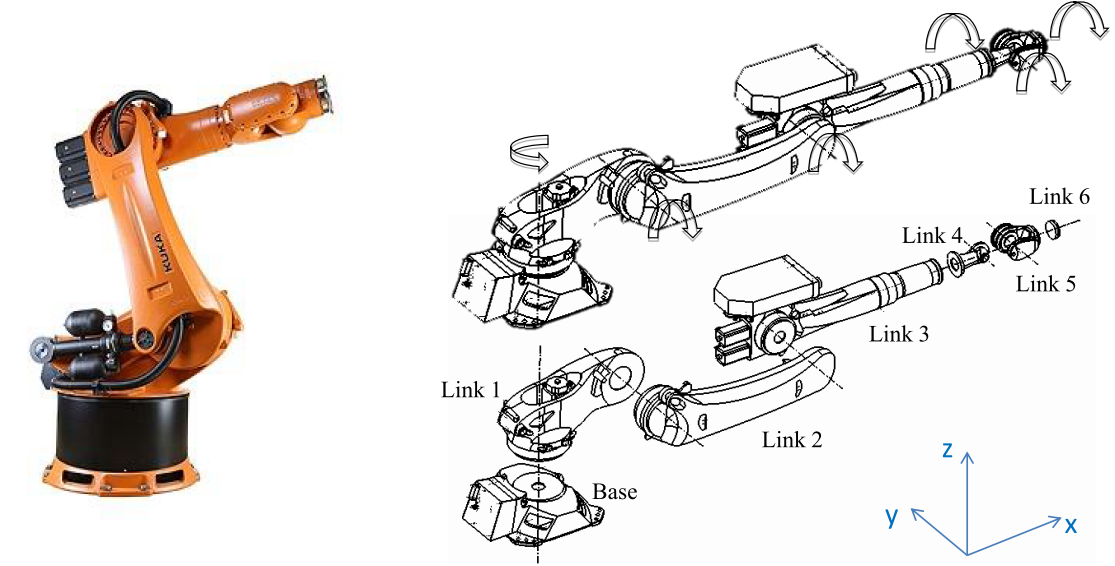
\includegraphics[height=2.5cm,width=\textwidth,keepaspectratio]{skillbox_task6/skillbox_la8_slide10_kuka.png}
    \large
    \setlength{\jot}{1pt}
    \begin{align*}
        \mathbf{T}
        &= \mathbf{T}_{\mathrm{Base}}\,T_z(d_0)\,\mathbf{A}\,\mathbf{W}\,T_x(d_6)\,\mathbf{T}_{\mathrm{Tool}}, \\
        \mathbf{A}
        &= R_z(q_1)T_x(d_1)R_y(q_2)T_x(d_2) \\
        &\quad {}\cdot R_y(q_3)T_x(d_3)T_z(d_4), \\
        \mathbf{W}
        &= R_x(q_4)R_y(q_5)R_x(q_6).
    \end{align*}
    \normalsize
    $\mathbf{A}$: robot manipulator; $\mathbf{W}$: robot wrist.
\end{frame}

\begin{frame}[t]{Changing Basis}
    \framesubtitle{Task 4}
    \only<1>{
        \begin{columns}[T,onlytextwidth]
            \begin{column}{0.54\textwidth}
                \begin{figure}[H]
                    \centering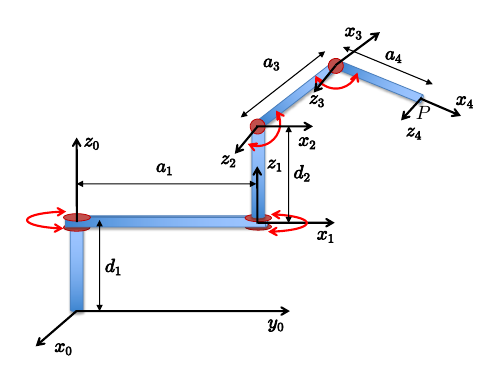
\includegraphics[height=4.7cm,width=\textwidth,keepaspectratio]{skillbox_task6/mod2_video8_task1_robot.png}
                \end{figure}
            \end{column}
            \begin{column}{0.44\textwidth}
                Find the homogeneous transformation matrix
                ${}^{0}\mathbf{T}_{4}$ for the robot shown.
                \medskip

                \textbf{Given:}
                \begin{itemize}
                    \item Link dimensions: $d_1$, $a_1$, $d_2$, $a_3$, $a_4$.
                    \item Joint angles: $\theta_1$, $\theta_2$, $\theta_3$, $\theta_4$.
                \end{itemize}
                \medskip
                The matrix maps coordinates from frame $4$ to frame $0$:
                \[
                    {}^{0}\bar{\mathbf{p}}
                    ={}^{0}\mathbf{T}_{4}\,{}^{4}\bar{\mathbf{p}}.
                \]
            \end{column}
        \end{columns}
    }
    \only<2>{
        \alert{\Large Answer}
        \medskip

        Following the frames from the base to the end of the arm:
        \begin{align*}
            {}^{0}\mathbf{T}_{1}
            &= T_z(d_1)R_z(90^{\circ})R_z(\theta_1)T_x(a_1), \\
            {}^{1}\mathbf{T}_{2}
            &= R_z(\theta_2)T_z(d_2)R_x(90^{\circ}), \\
            {}^{2}\mathbf{T}_{3}
            &= R_z(\theta_3)T_x(a_3), \\
            {}^{3}\mathbf{T}_{4}
            &= R_z(\theta_4)T_x(a_4).
        \end{align*}
        \medskip
        \[
            \boxed{{}^{0}\mathbf{T}_{4}
            ={}^{0}\mathbf{T}_{1}\,{}^{1}\mathbf{T}_{2}\,
             {}^{2}\mathbf{T}_{3}\,{}^{3}\mathbf{T}_{4}}
        \]
        \medskip
        $T_x,T_z$: translations; $R_x,R_z$: rotations.
    }
    \only<3>{
        \alert{\Large Answer}
        \medskip

        Let $s_i=\sin\theta_i$, $c_i=\cos\theta_i$,
        $s_{ij}=\sin(\theta_i+\theta_j)$,
        $c_{ij}=\cos(\theta_i+\theta_j)$.
        \medskip
        \[
            {}^{0}\mathbf{T}_{4}=
            \begin{bmatrix}
                -s_{12}c_{34} & s_{12}s_{34} & c_{12} & p_x \\
                 c_{12}c_{34} & -c_{12}s_{34} & s_{12} & p_y \\
                 s_{34} & c_{34} & 0 & p_z \\
                 0 & 0 & 0 & 1
            \end{bmatrix},
        \]
        \begin{align*}
            p_x &= -a_1s_1-s_{12}(a_3c_3+a_4c_{34}), \\
            p_y &= \phantom{-}a_1c_1+c_{12}(a_3c_3+a_4c_{34}), \\
            p_z &= d_1+d_2+a_3s_3+a_4s_{34}.
        \end{align*}
    }
\end{frame}




\begin{frame}[t]{Reference Materials}
    \begin{itemize}
        \item A. De Luca --- 01 IndustrialRobots
        \item A. Klimchik --- L1 Introduction
        \item Skillbox --- Prik linal 7
        \item Skillbox --- Mod2 latex text
        \item Skillbox --- Mod2
        \item Skillbox --- Prik linal 8
    \end{itemize}
\end{frame}

\fbckg{fibeamer/figs/last_page.png}
\frame[plain]{}

\end{document}
